\documentclass[../main.tex]{subfiles}

\begin{document}

\setcounter{chapter}{2}

\chapter{数据通路实验}

\section{实验目的}

\begin{enumerate}

    \item 进一步熟悉 TEC-8 模型计算机的数据通路的结构;
    \item 进一步掌握数据通路中各个控制信号的作用和用法;
    \item 掌握数据通路中数据流动的路径.

\end{enumerate}

\section{实验内容}

\begin{enumerate}

    \item 将数 75H 写到寄存器 R$_0$, 数 28H 写道寄存器 R$_1$, 数 89H 写到寄存器 R$_2$, 数 32H 写到寄存器 R$_3$.
    \item 将寄存器 R$_0$ 中的数写入存储器 20H 单元, 将寄存器 R$_1$ 中的数写入存储器 21H 单元, 将寄存器 R$_2$ 中的数写入存储器 22H 单元, 将寄存器 R$_3$ 中的数写入存储器 23H 单元.
    \item 从存储器 20H 单元读出数到存储器 R$_3$, 从存储器 21H 单元读出数到存储器 R$_2$, 从存储器21H 单元读出数到存储器 R$_1$, 从存储器 23H 单元读出数到存储器 R$_0$.
    \item 显示 4 个寄存器 R$_0$、R$_1$、R$_2$、R$_3$ 的值, 检查数据传送是否正确.

\end{enumerate}

\section{实验过程}

\subsection{微程序模式}

\begin{enumerate}

    \item 将控制器转换开关拨到微程序位置, 将编程开关设置为正常位置, 打开电源. 将操作模式开关设置为 SWC=1、SWB=1、SWA=1, 准备进入数据通路实验.

    \item 通过数据开关依次将数 75H 写到寄存器 R$_0$, 数 28H 写到 R$_1$, 数 89H 写到 R$_2$, 数 32H 写到 R$_3$. (如图 \ref{fig:3.1} 所示.)

          \begin{figure}[htbp]
              \centering
              \subfigure[将数 75H 写到 R$_0$]{
                  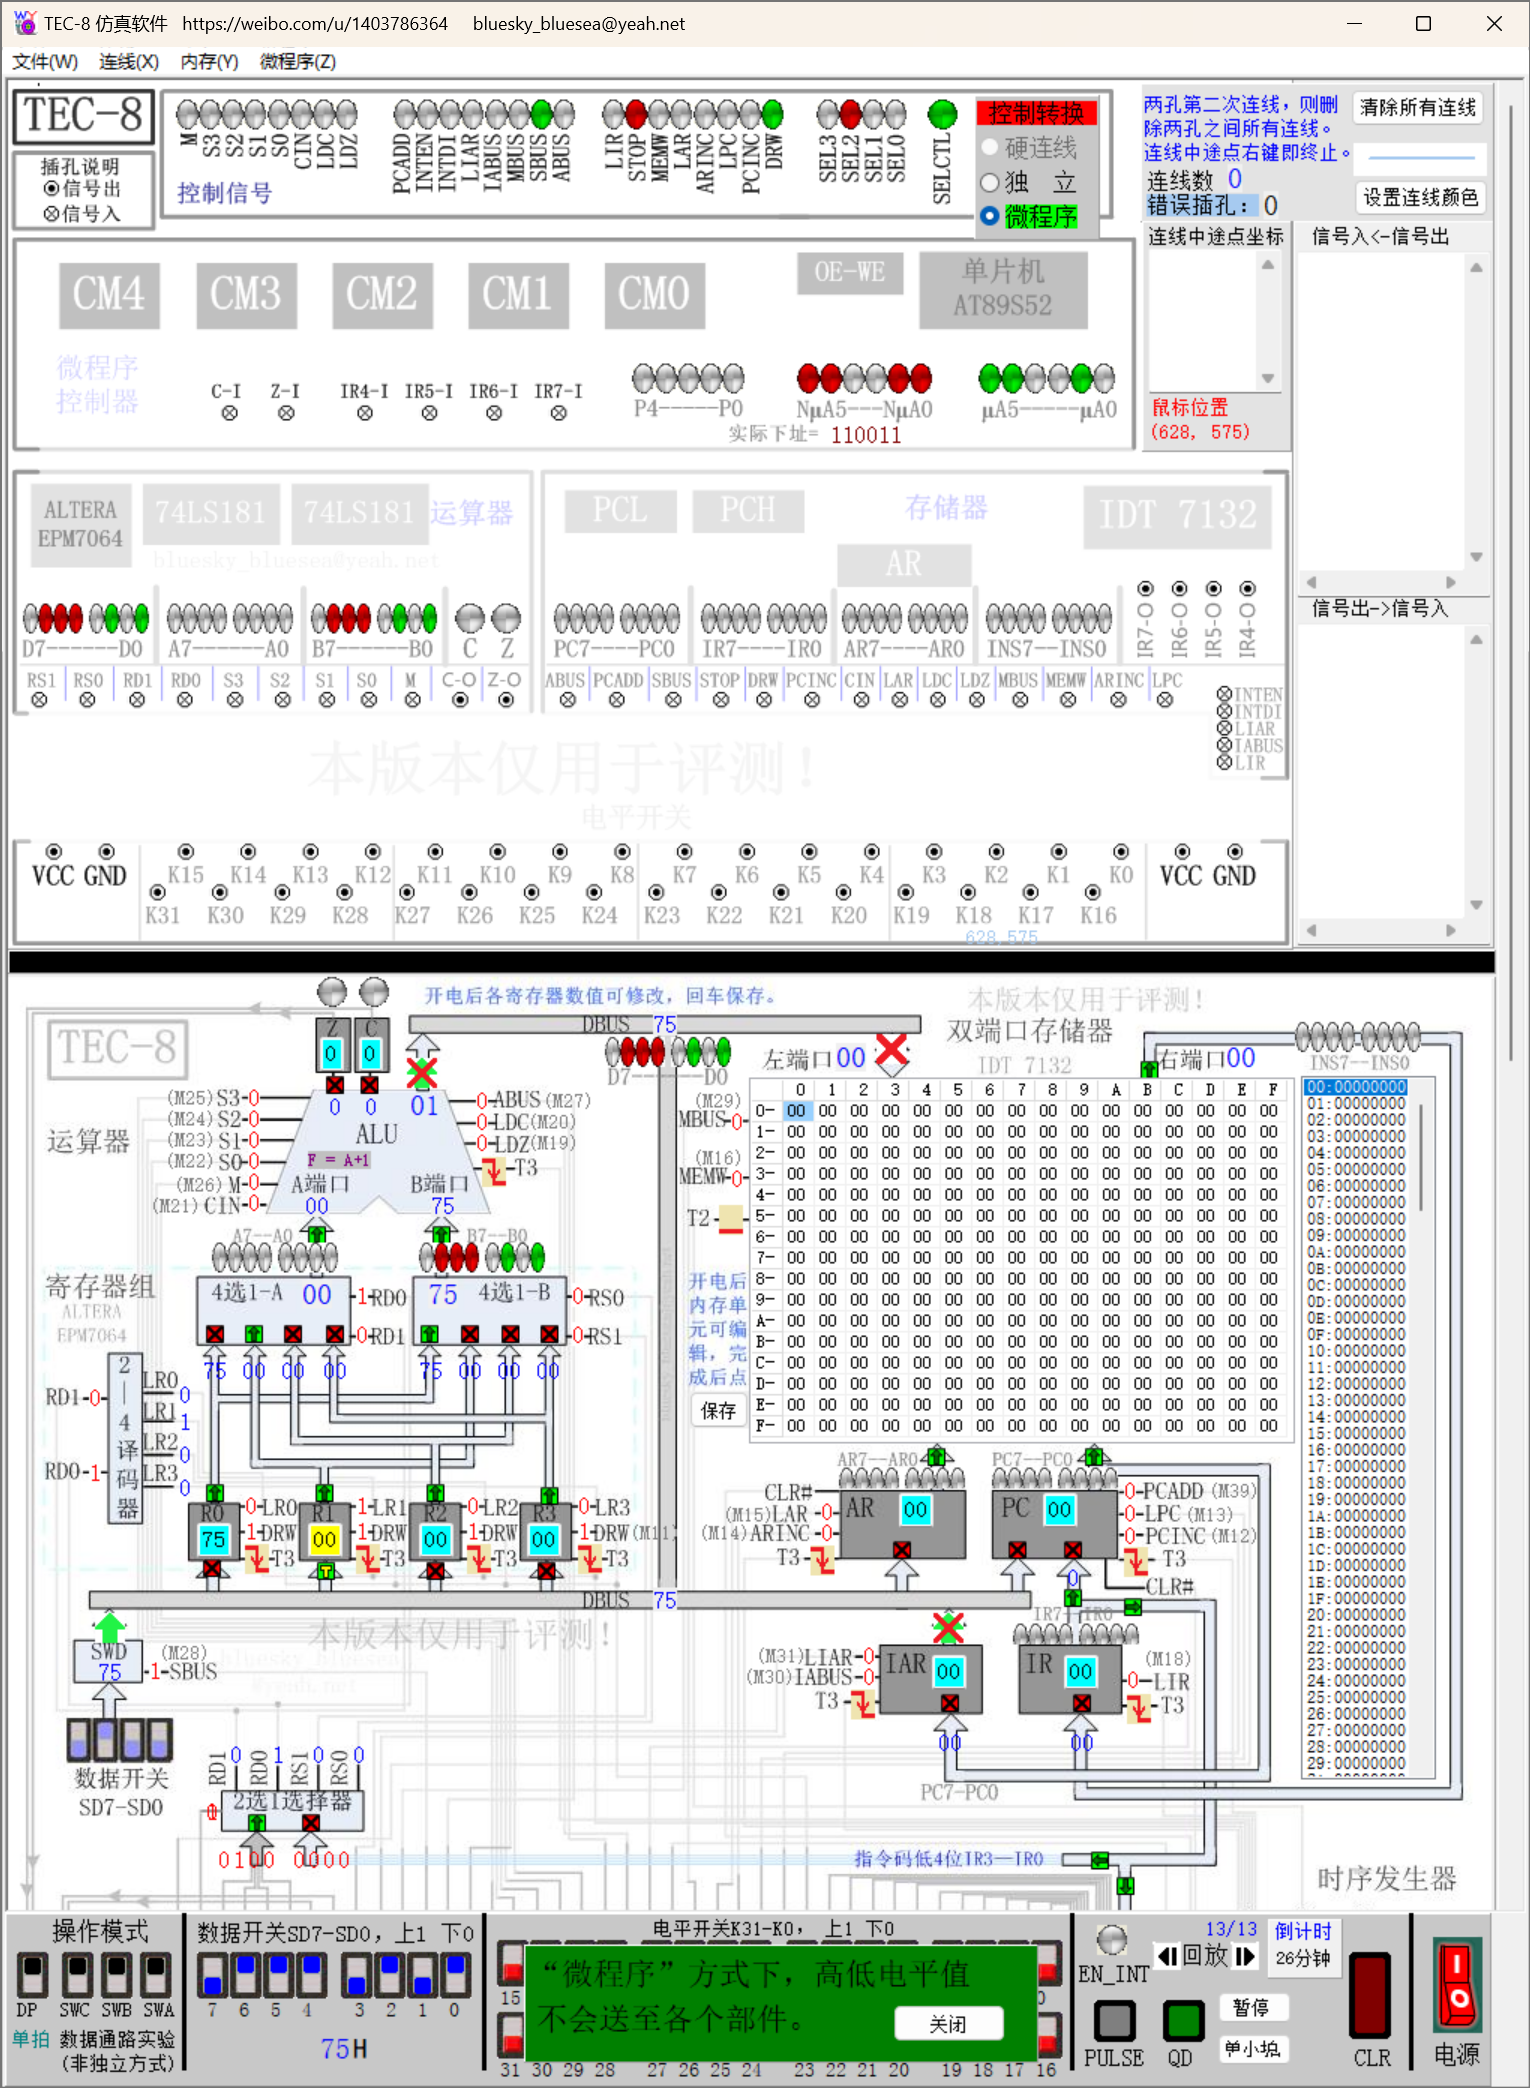
\includegraphics[width=0.3\textwidth]{screenshots/3.1.1.png}
              }
              \subfigure[将数 28H 写到 R$_1$]{
                  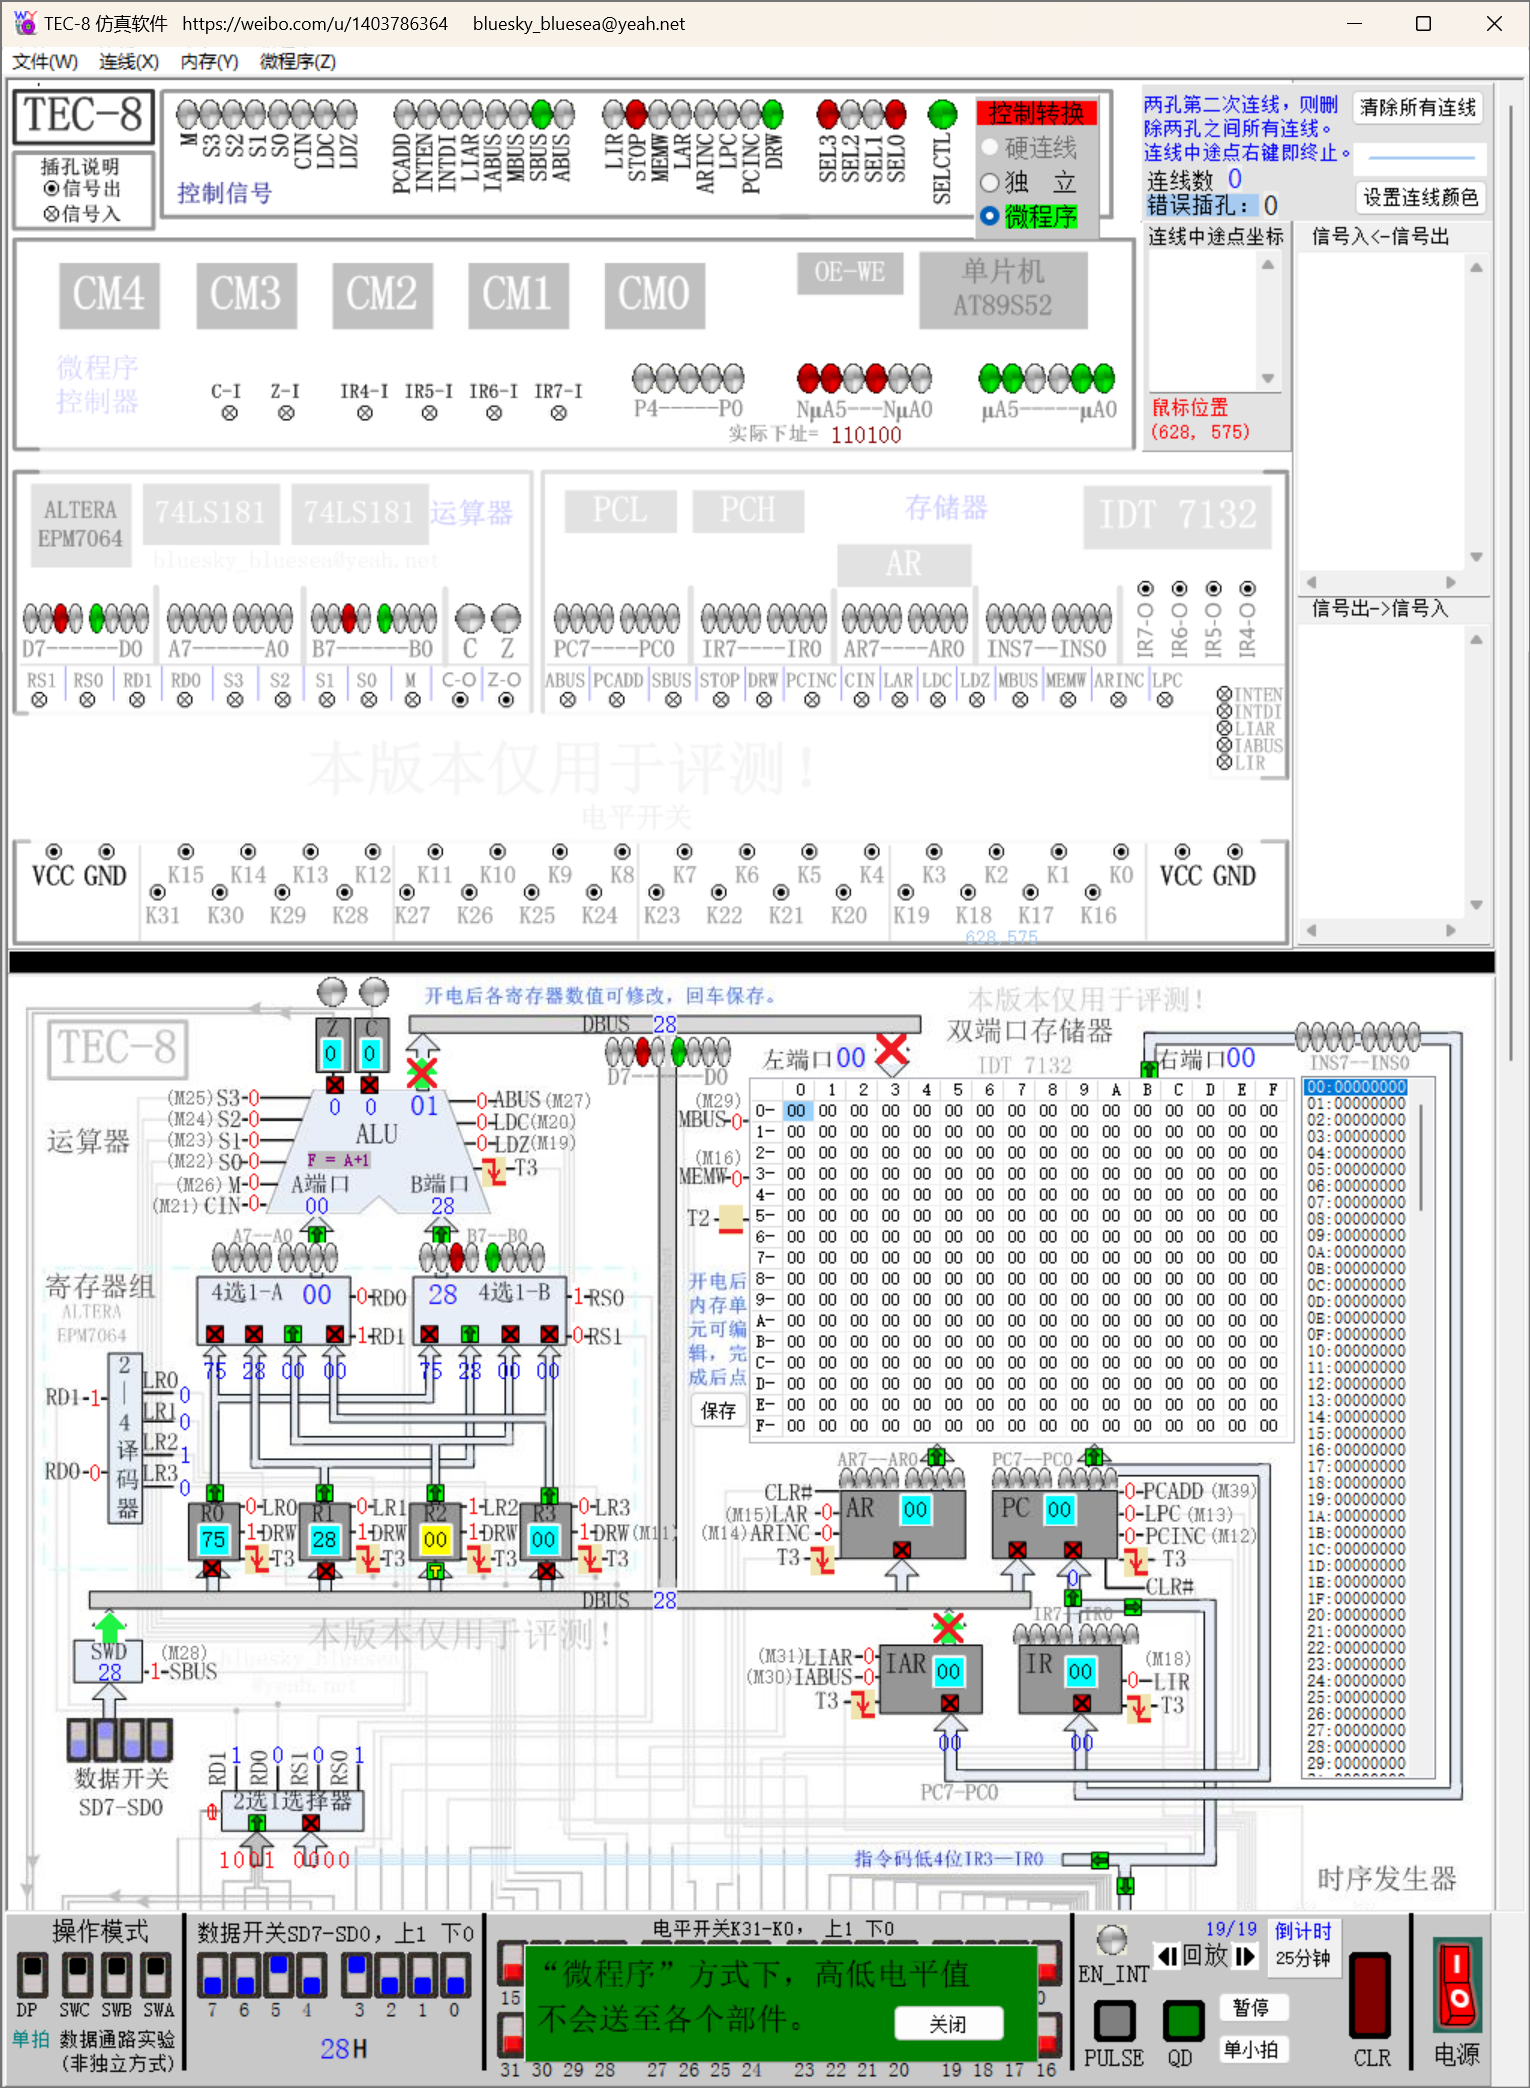
\includegraphics[width=0.3\textwidth]{screenshots/3.1.2.png}
              }
              \\
              \subfigure[将数 89H 写到 R$_2$]{
                  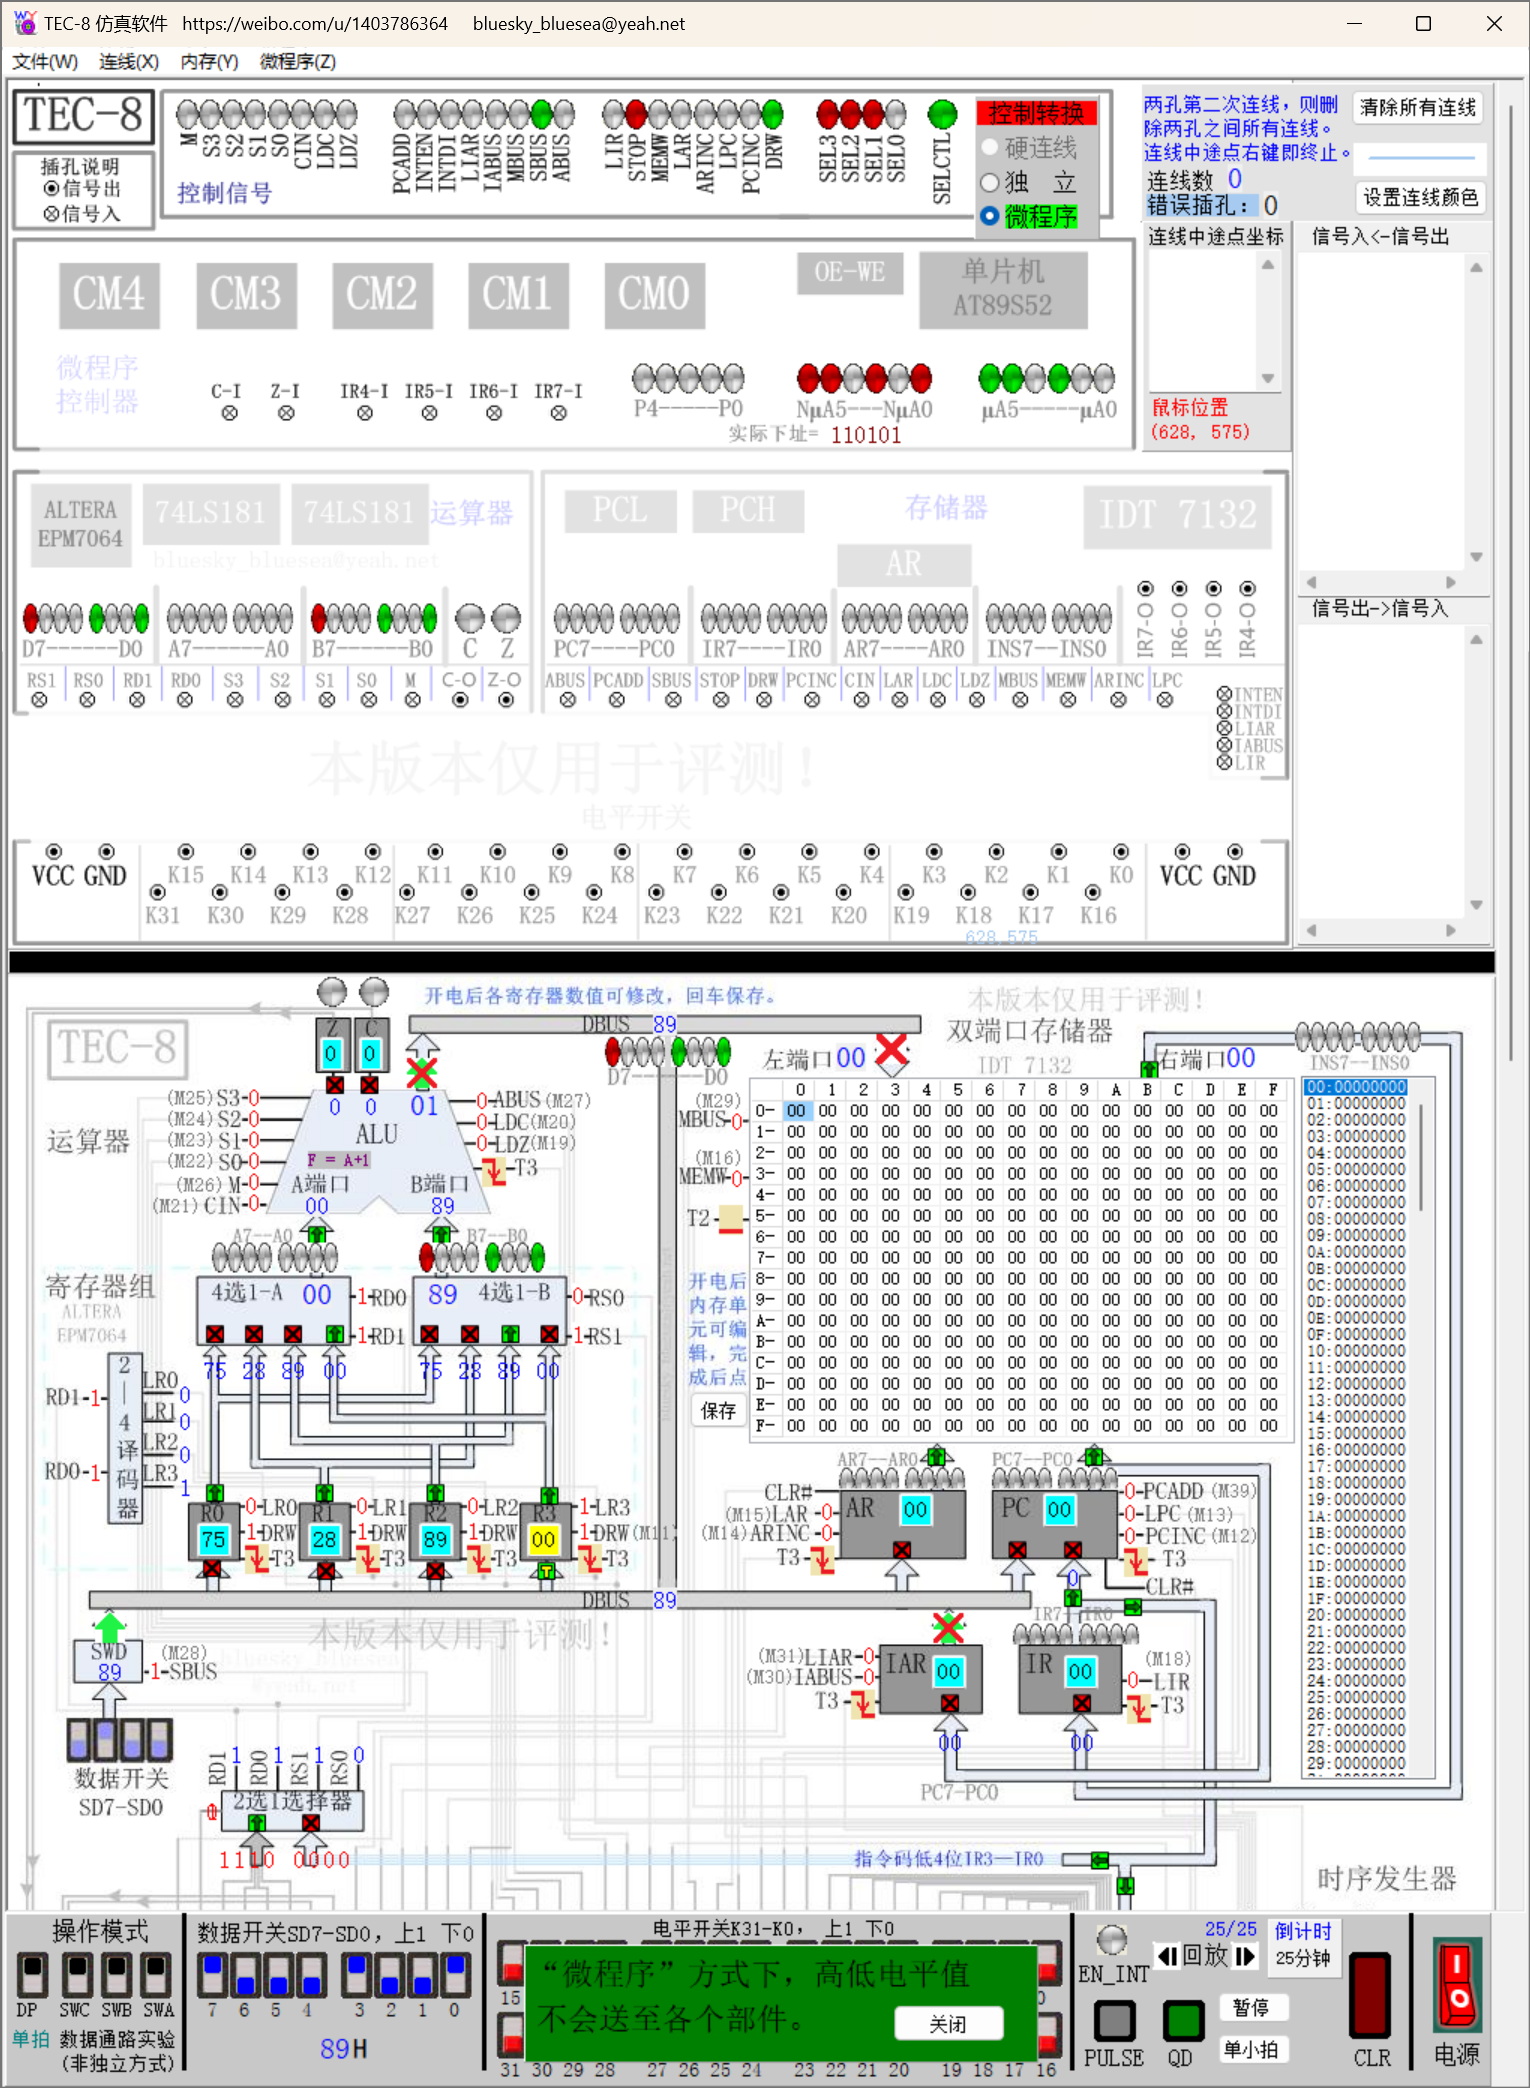
\includegraphics[width=0.3\textwidth]{screenshots/3.1.3.png}
              }
              \subfigure[将数 32H 写到 R$_3$]{
                  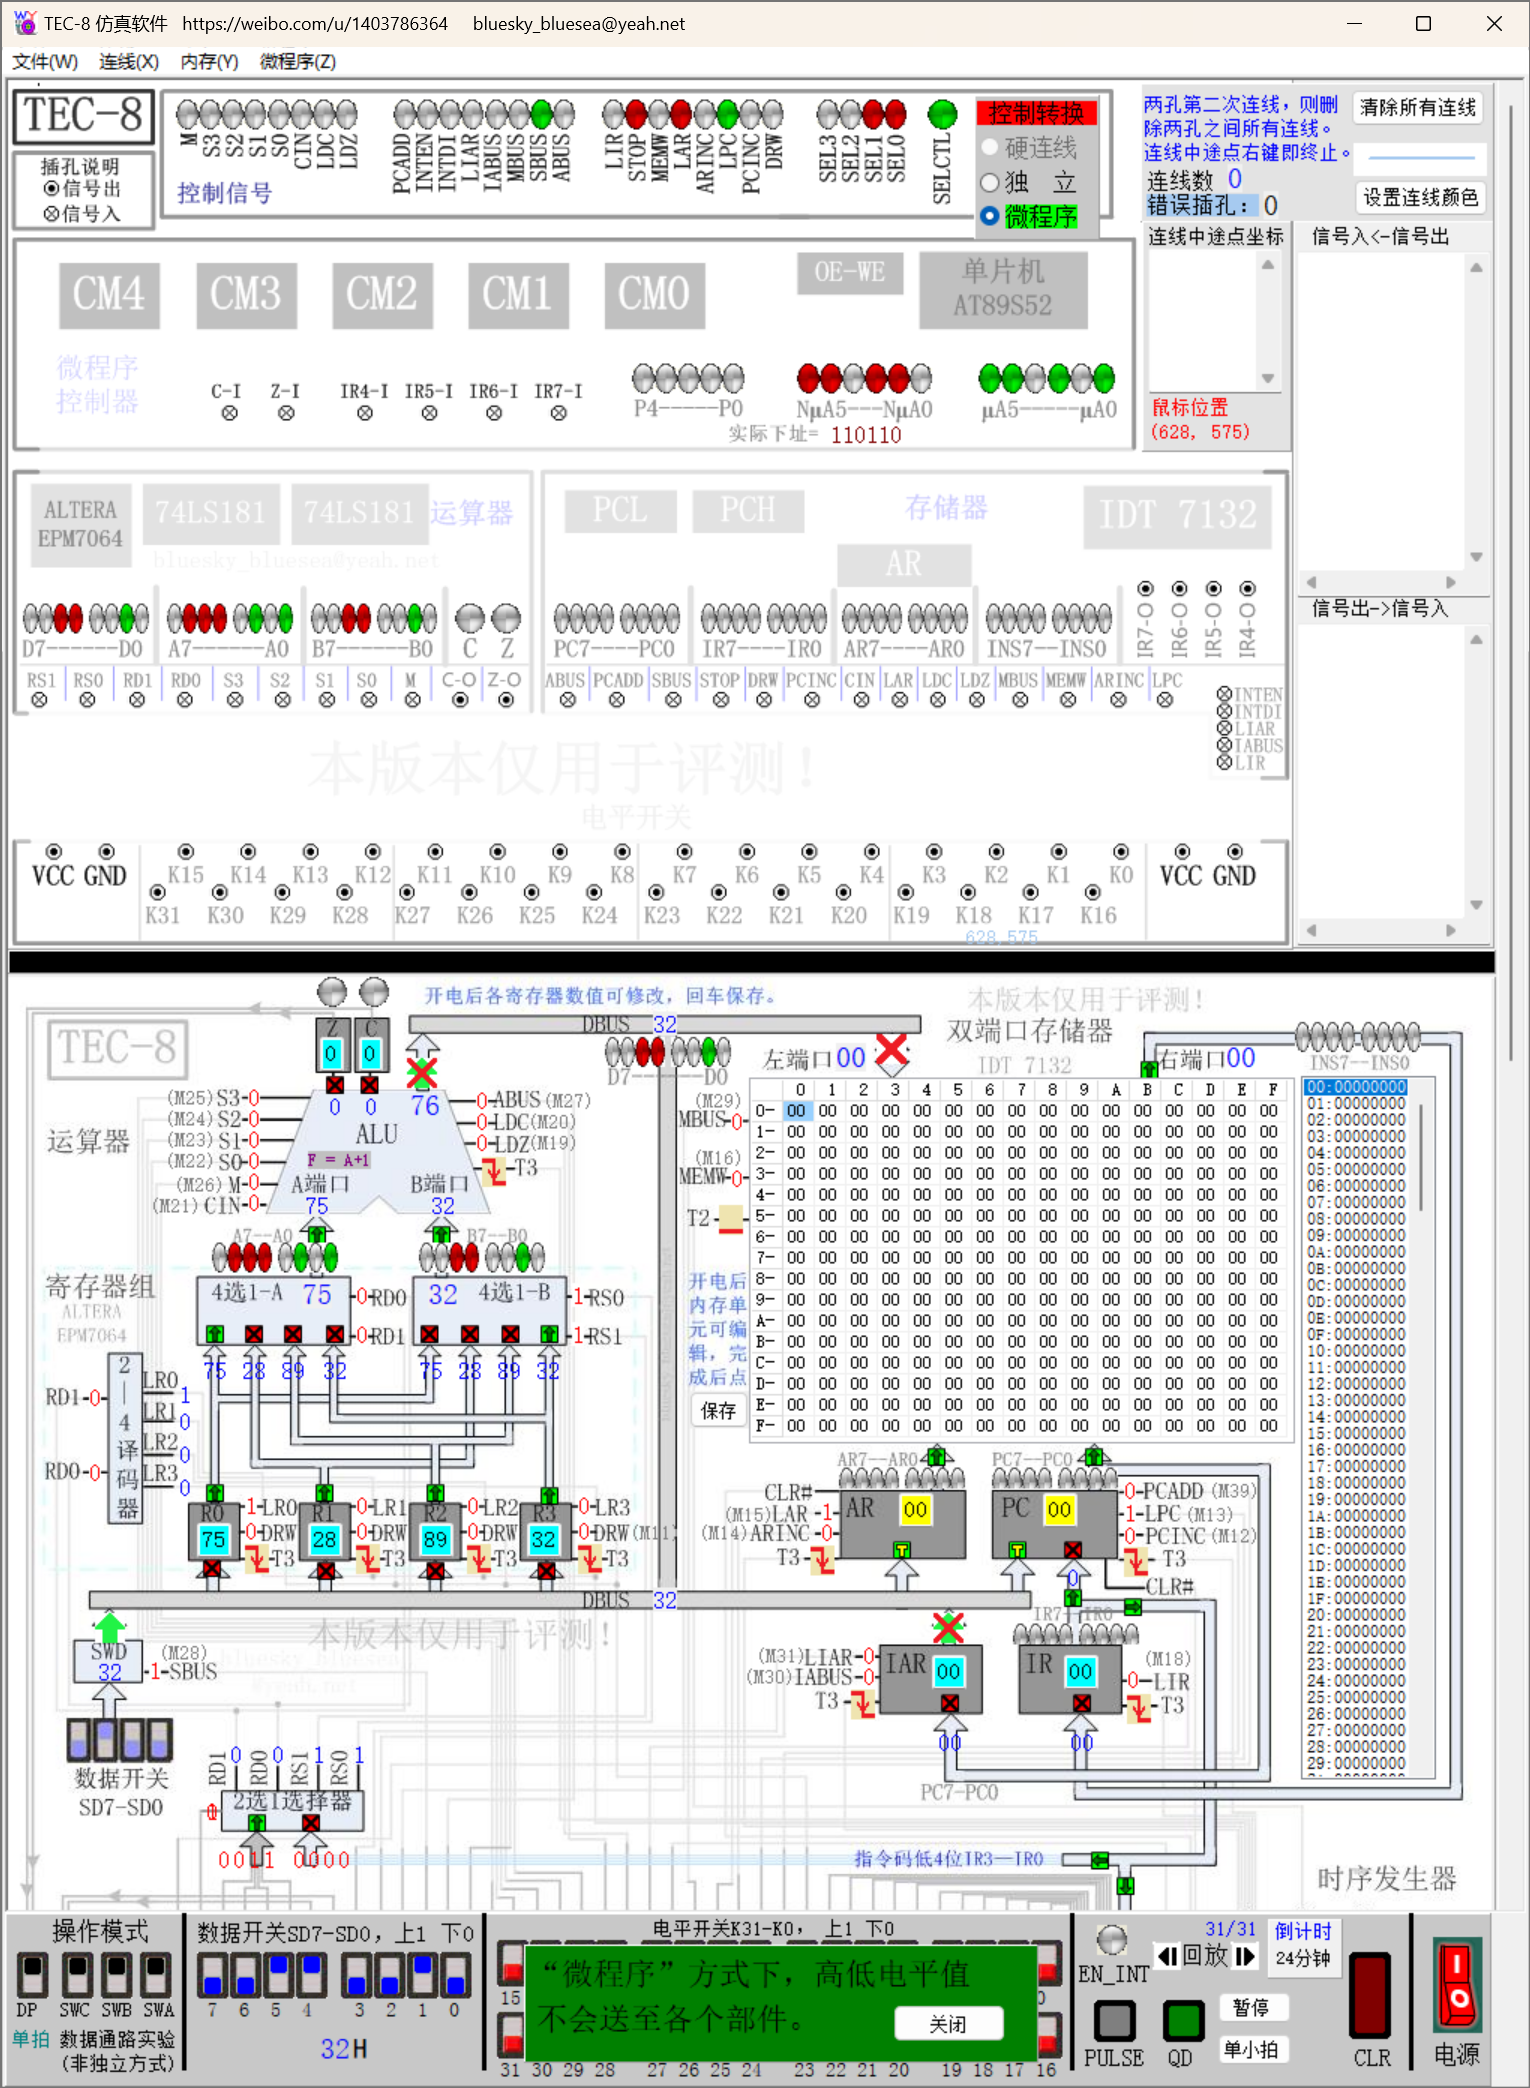
\includegraphics[width=0.3\textwidth]{screenshots/3.1.4.png}
              }
              \caption{写入数据 (微程序)}
              \label{fig:3.1}
          \end{figure}

    \item 设置存储器地址 AR 和程序计数器 PC 为 20H. (如图 \ref{fig:3.2} 所示.)

          \begin{figure}[htbp]
              \centering
              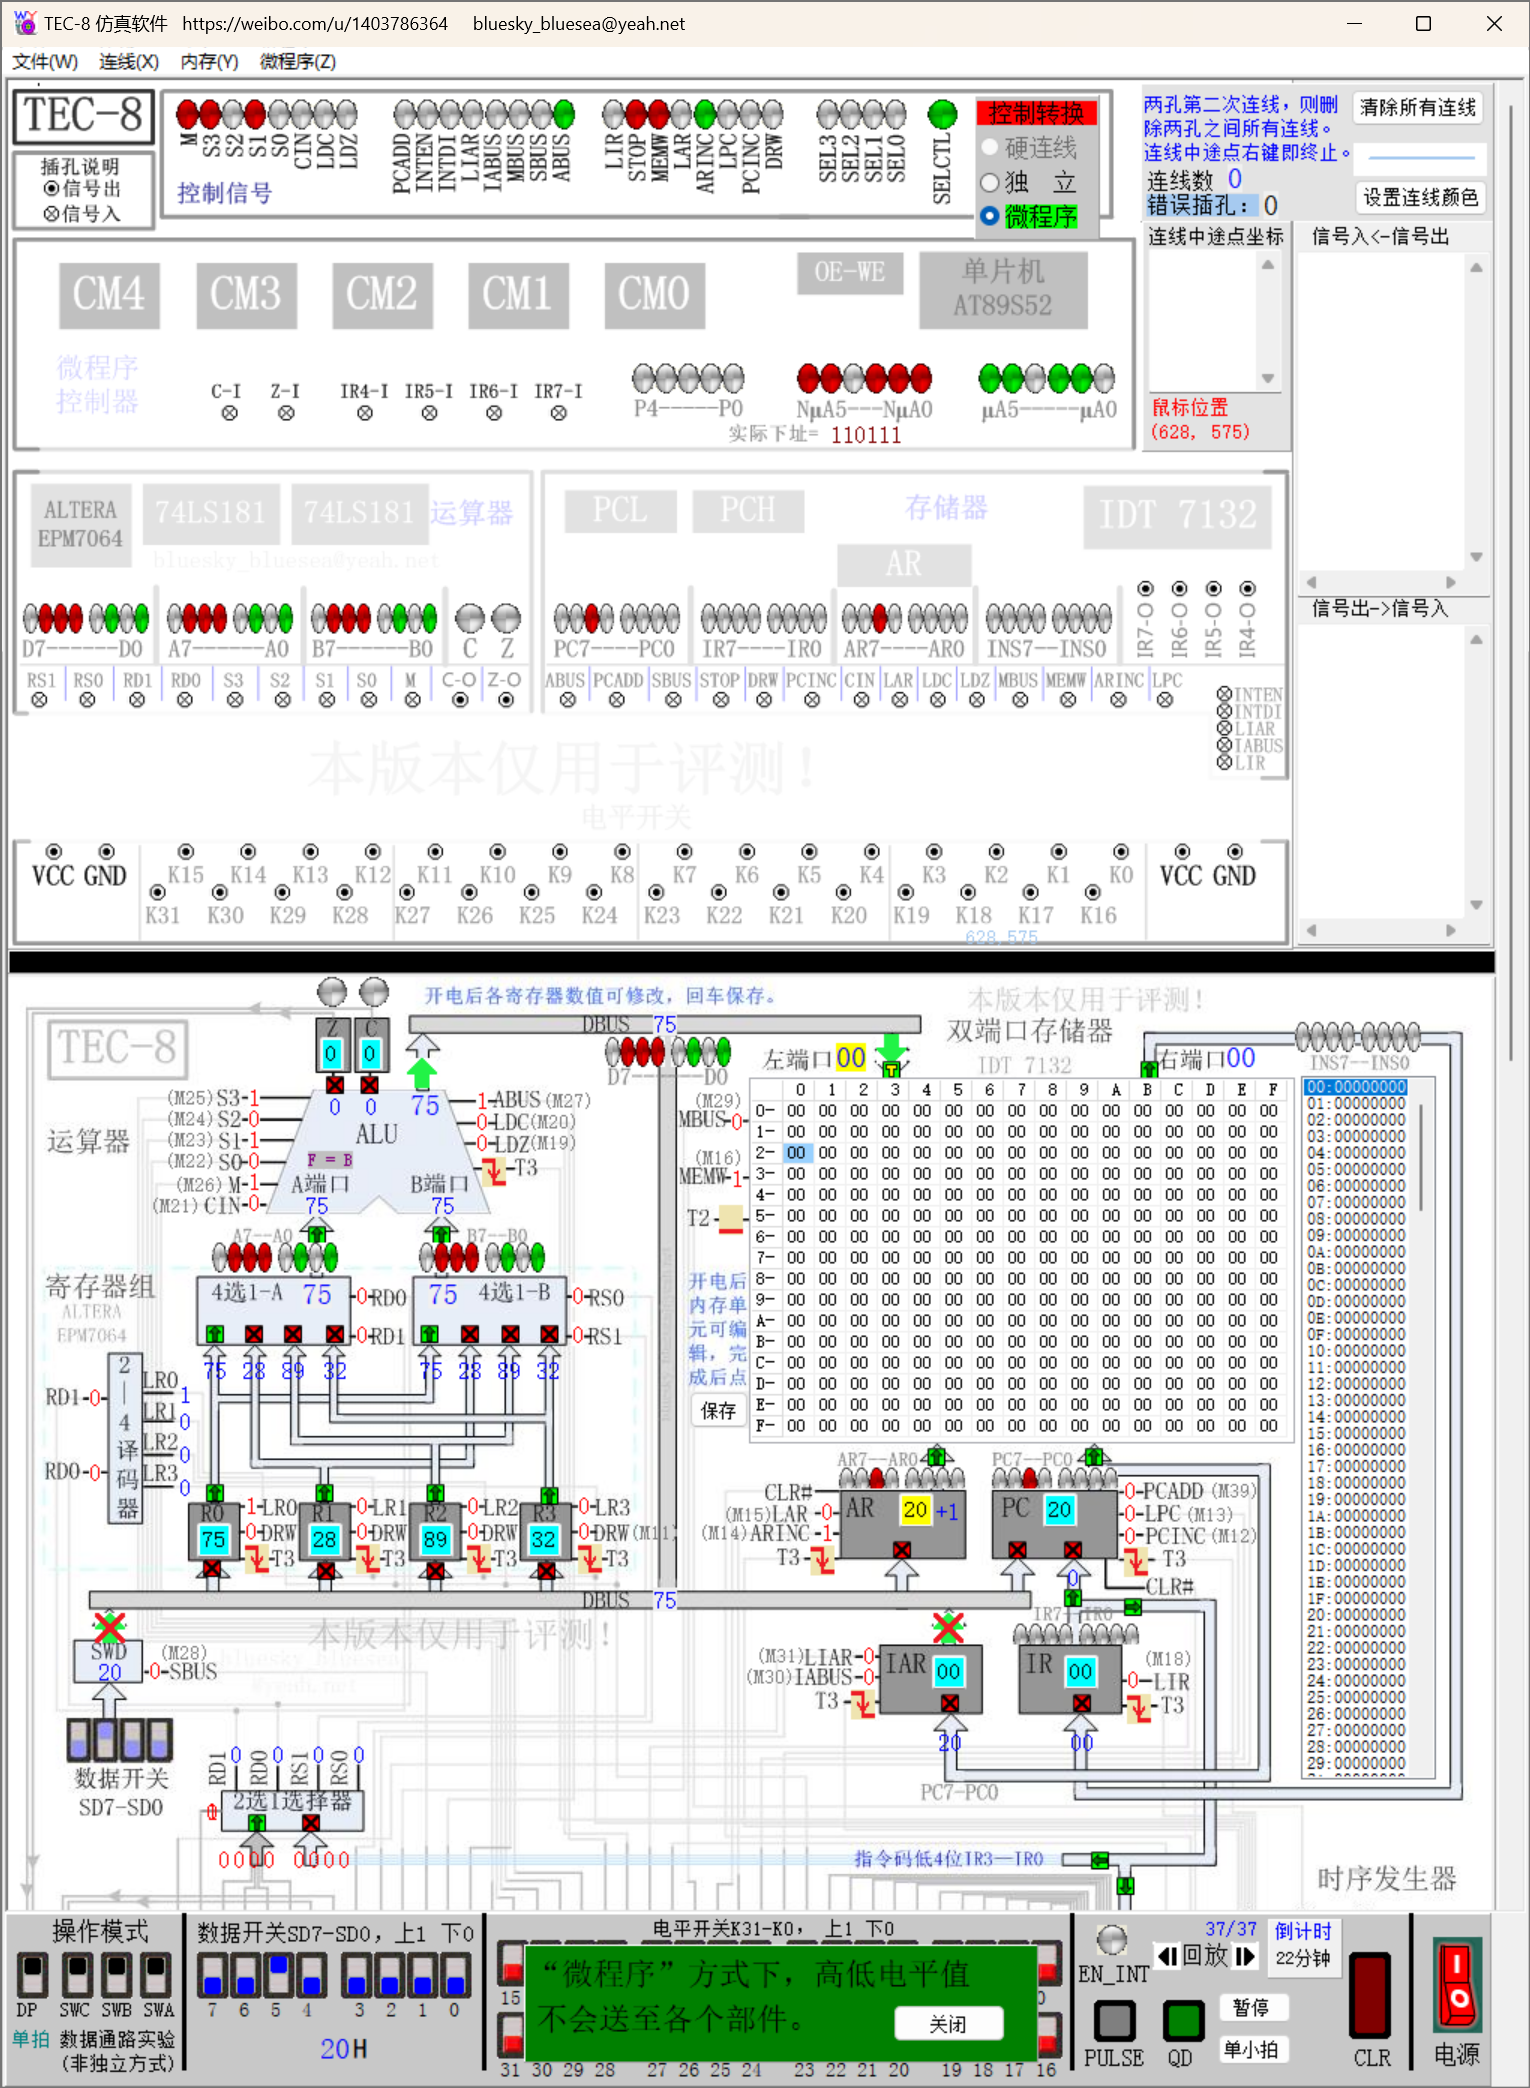
\includegraphics[width=0.3\textwidth]{screenshots/3.1.5.png}
              \caption{设置地址 (微程序)}
              \label{fig:3.2}
          \end{figure}

    \item 将寄存器 R$_0$、R$_1$、R$_2$、R$_3$ 中的数依次写入存储器 20H、21H、22H 和 23H 单元. (如图 \ref{fig:3.3} 所示.)

          \begin{figure}[htbp]
              \centering
              \subfigure[将R$_0$数值写入20H单元]{
                  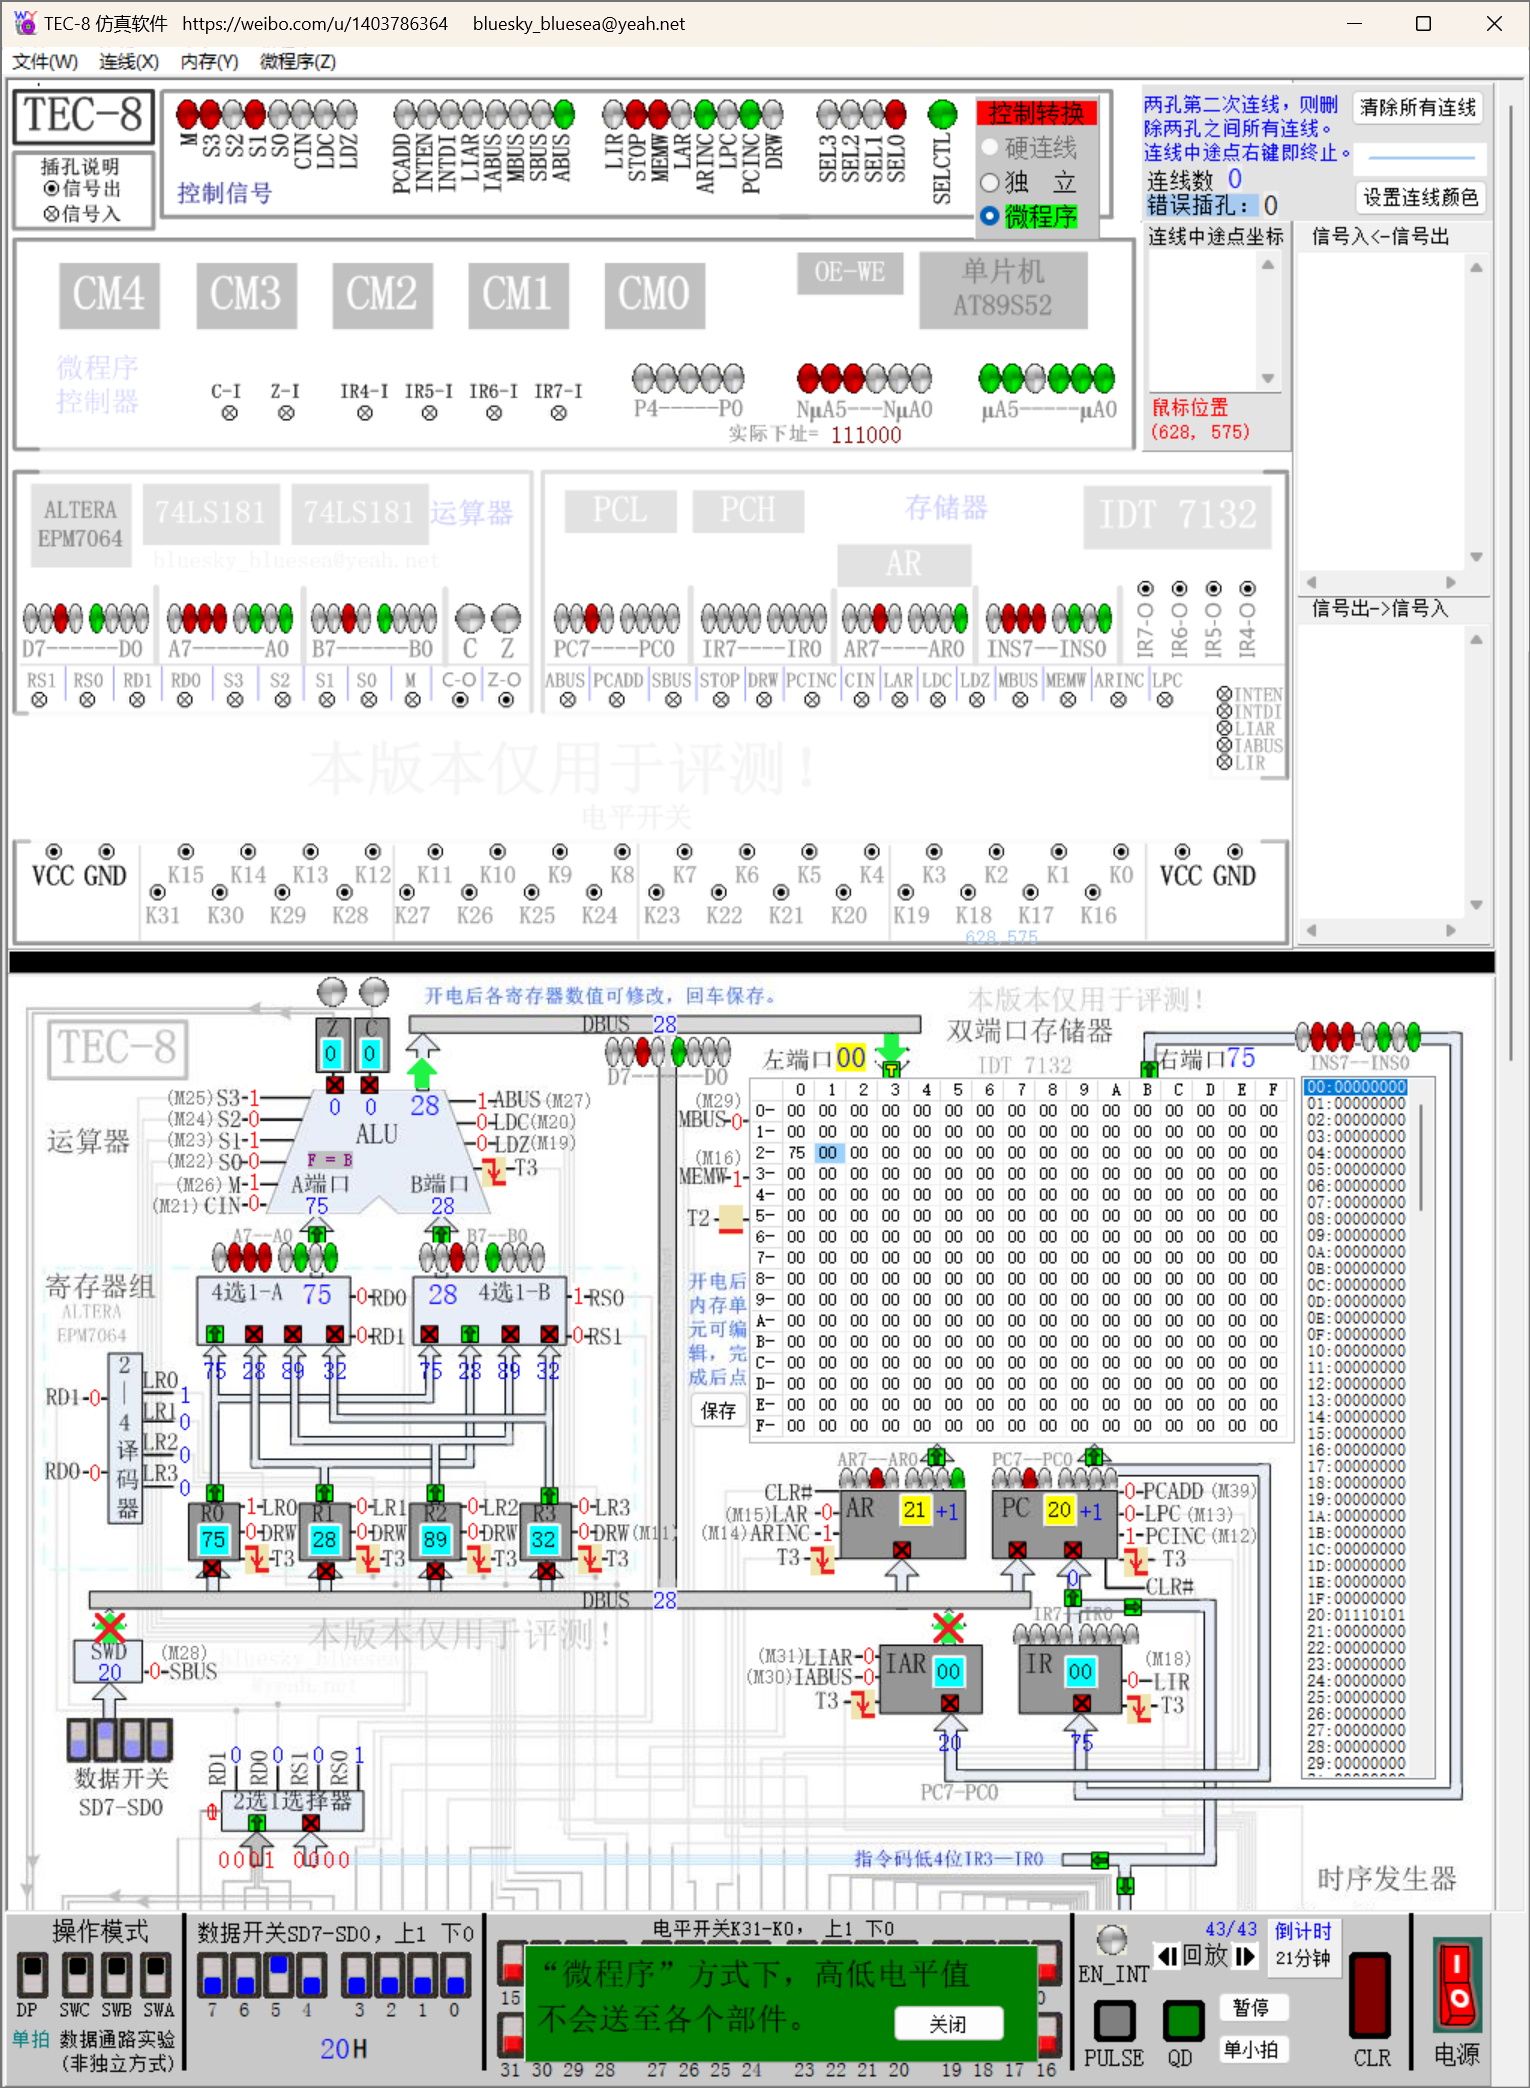
\includegraphics[width=0.3\textwidth]{screenshots/3.1.6.png}
              }
              \subfigure[将R$_1$数值写入21H单元]{
                  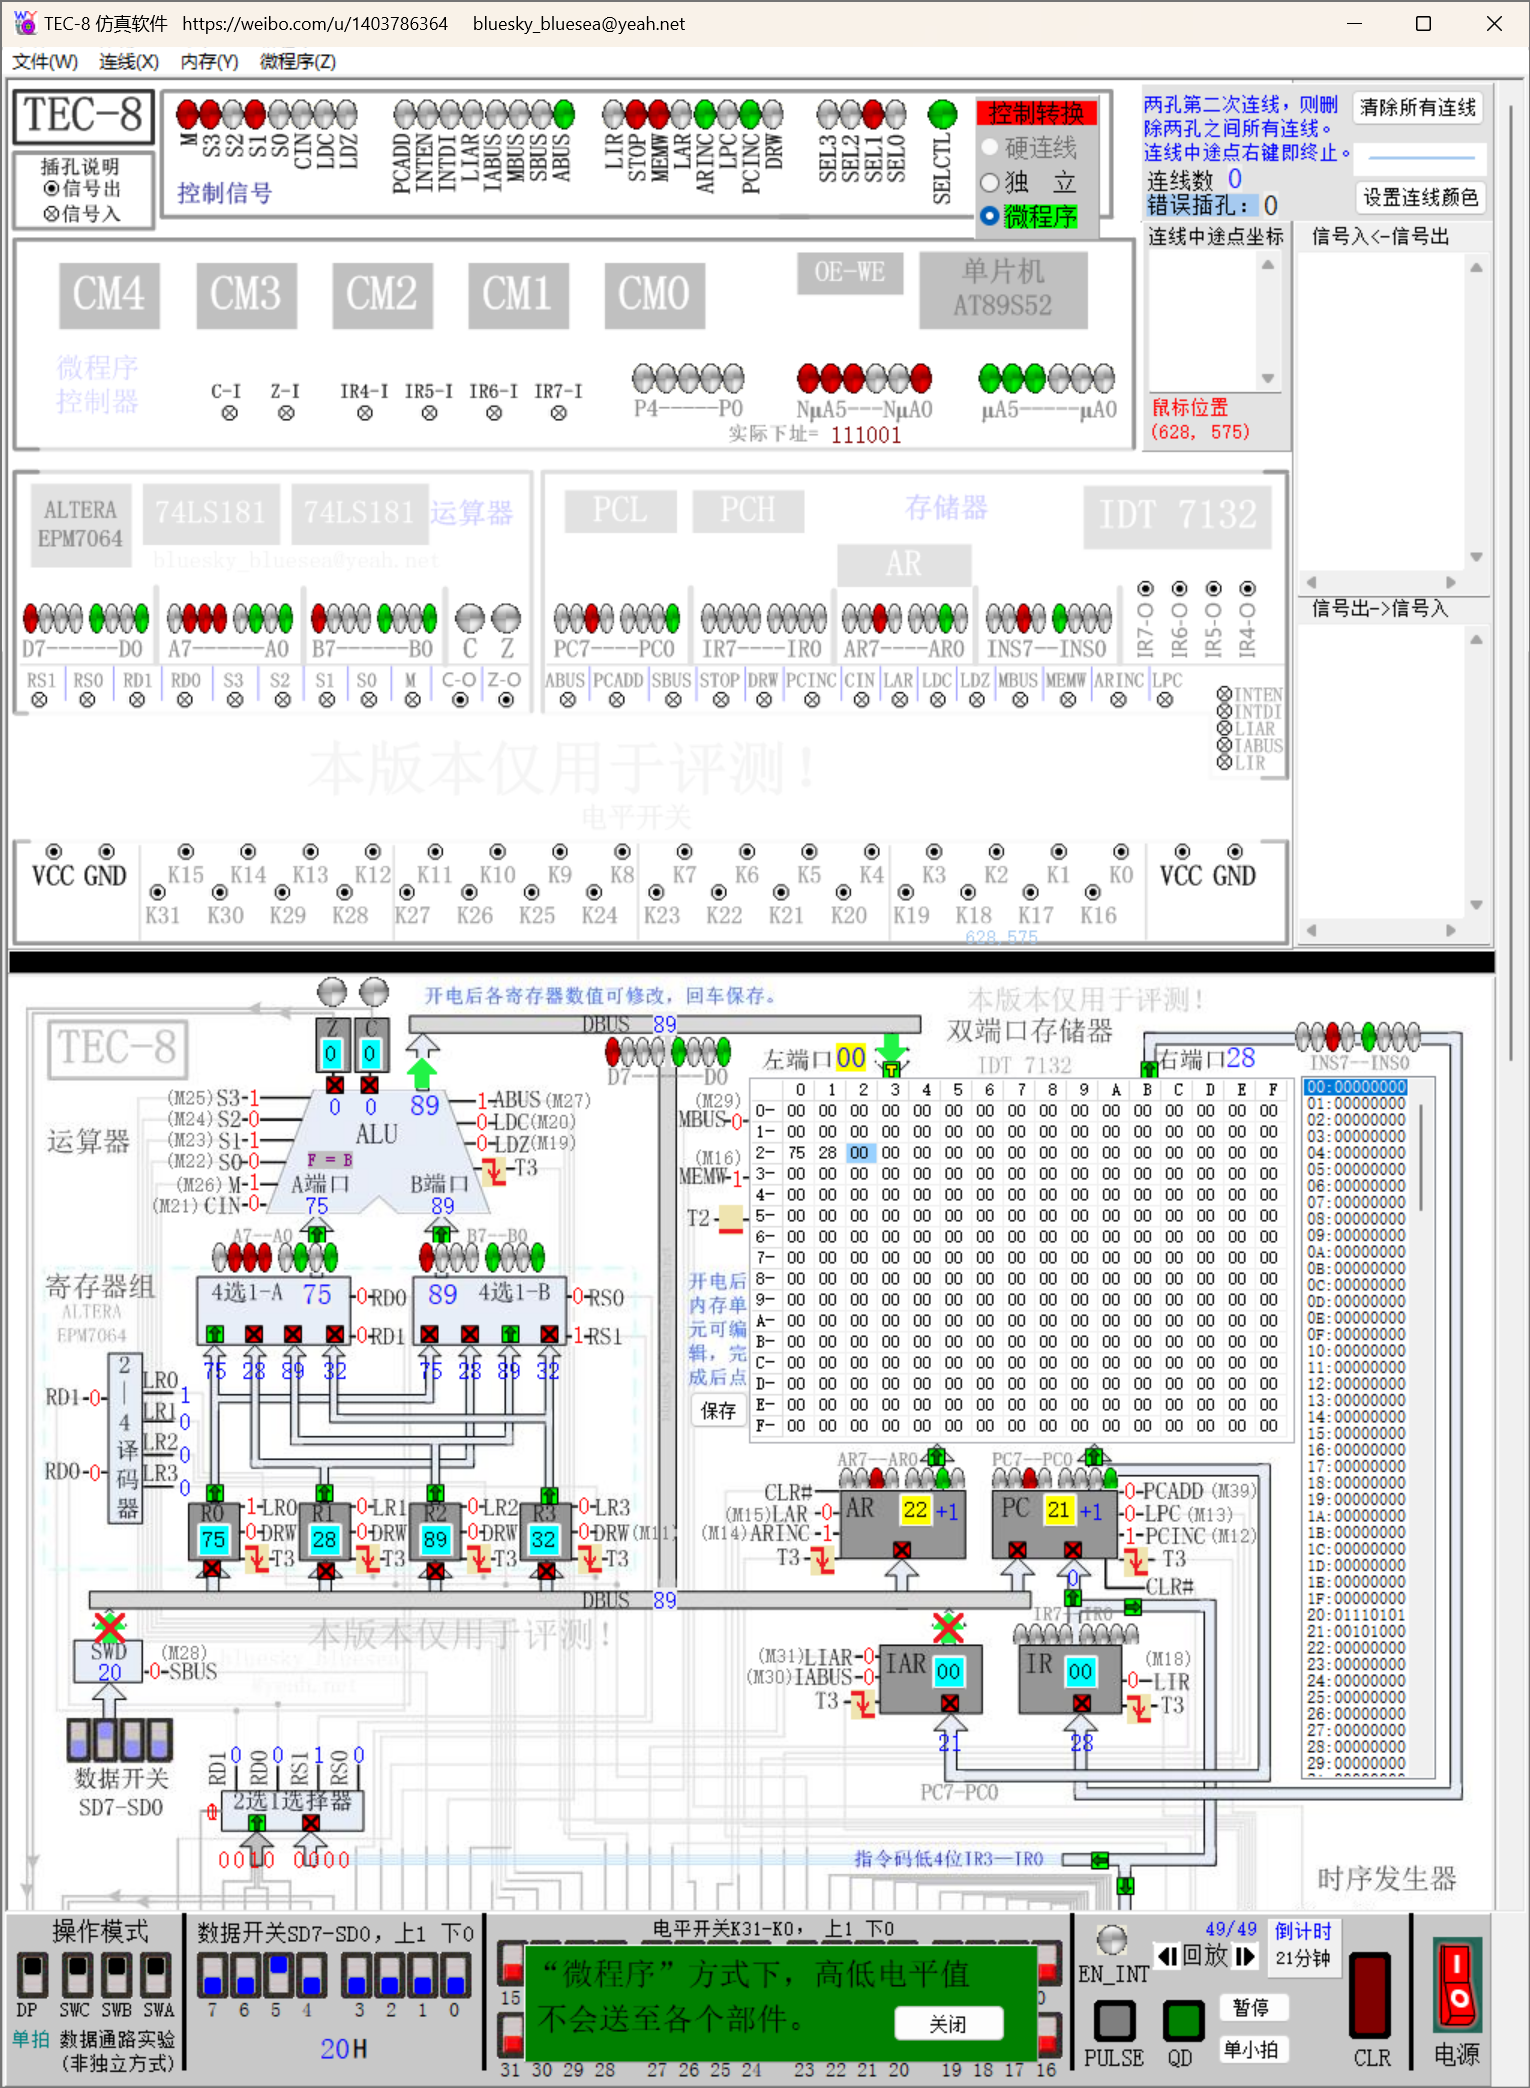
\includegraphics[width=0.3\textwidth]{screenshots/3.1.7.png}
              }
              \\
              \subfigure[将R$_2$数值写入22H单元]{
                  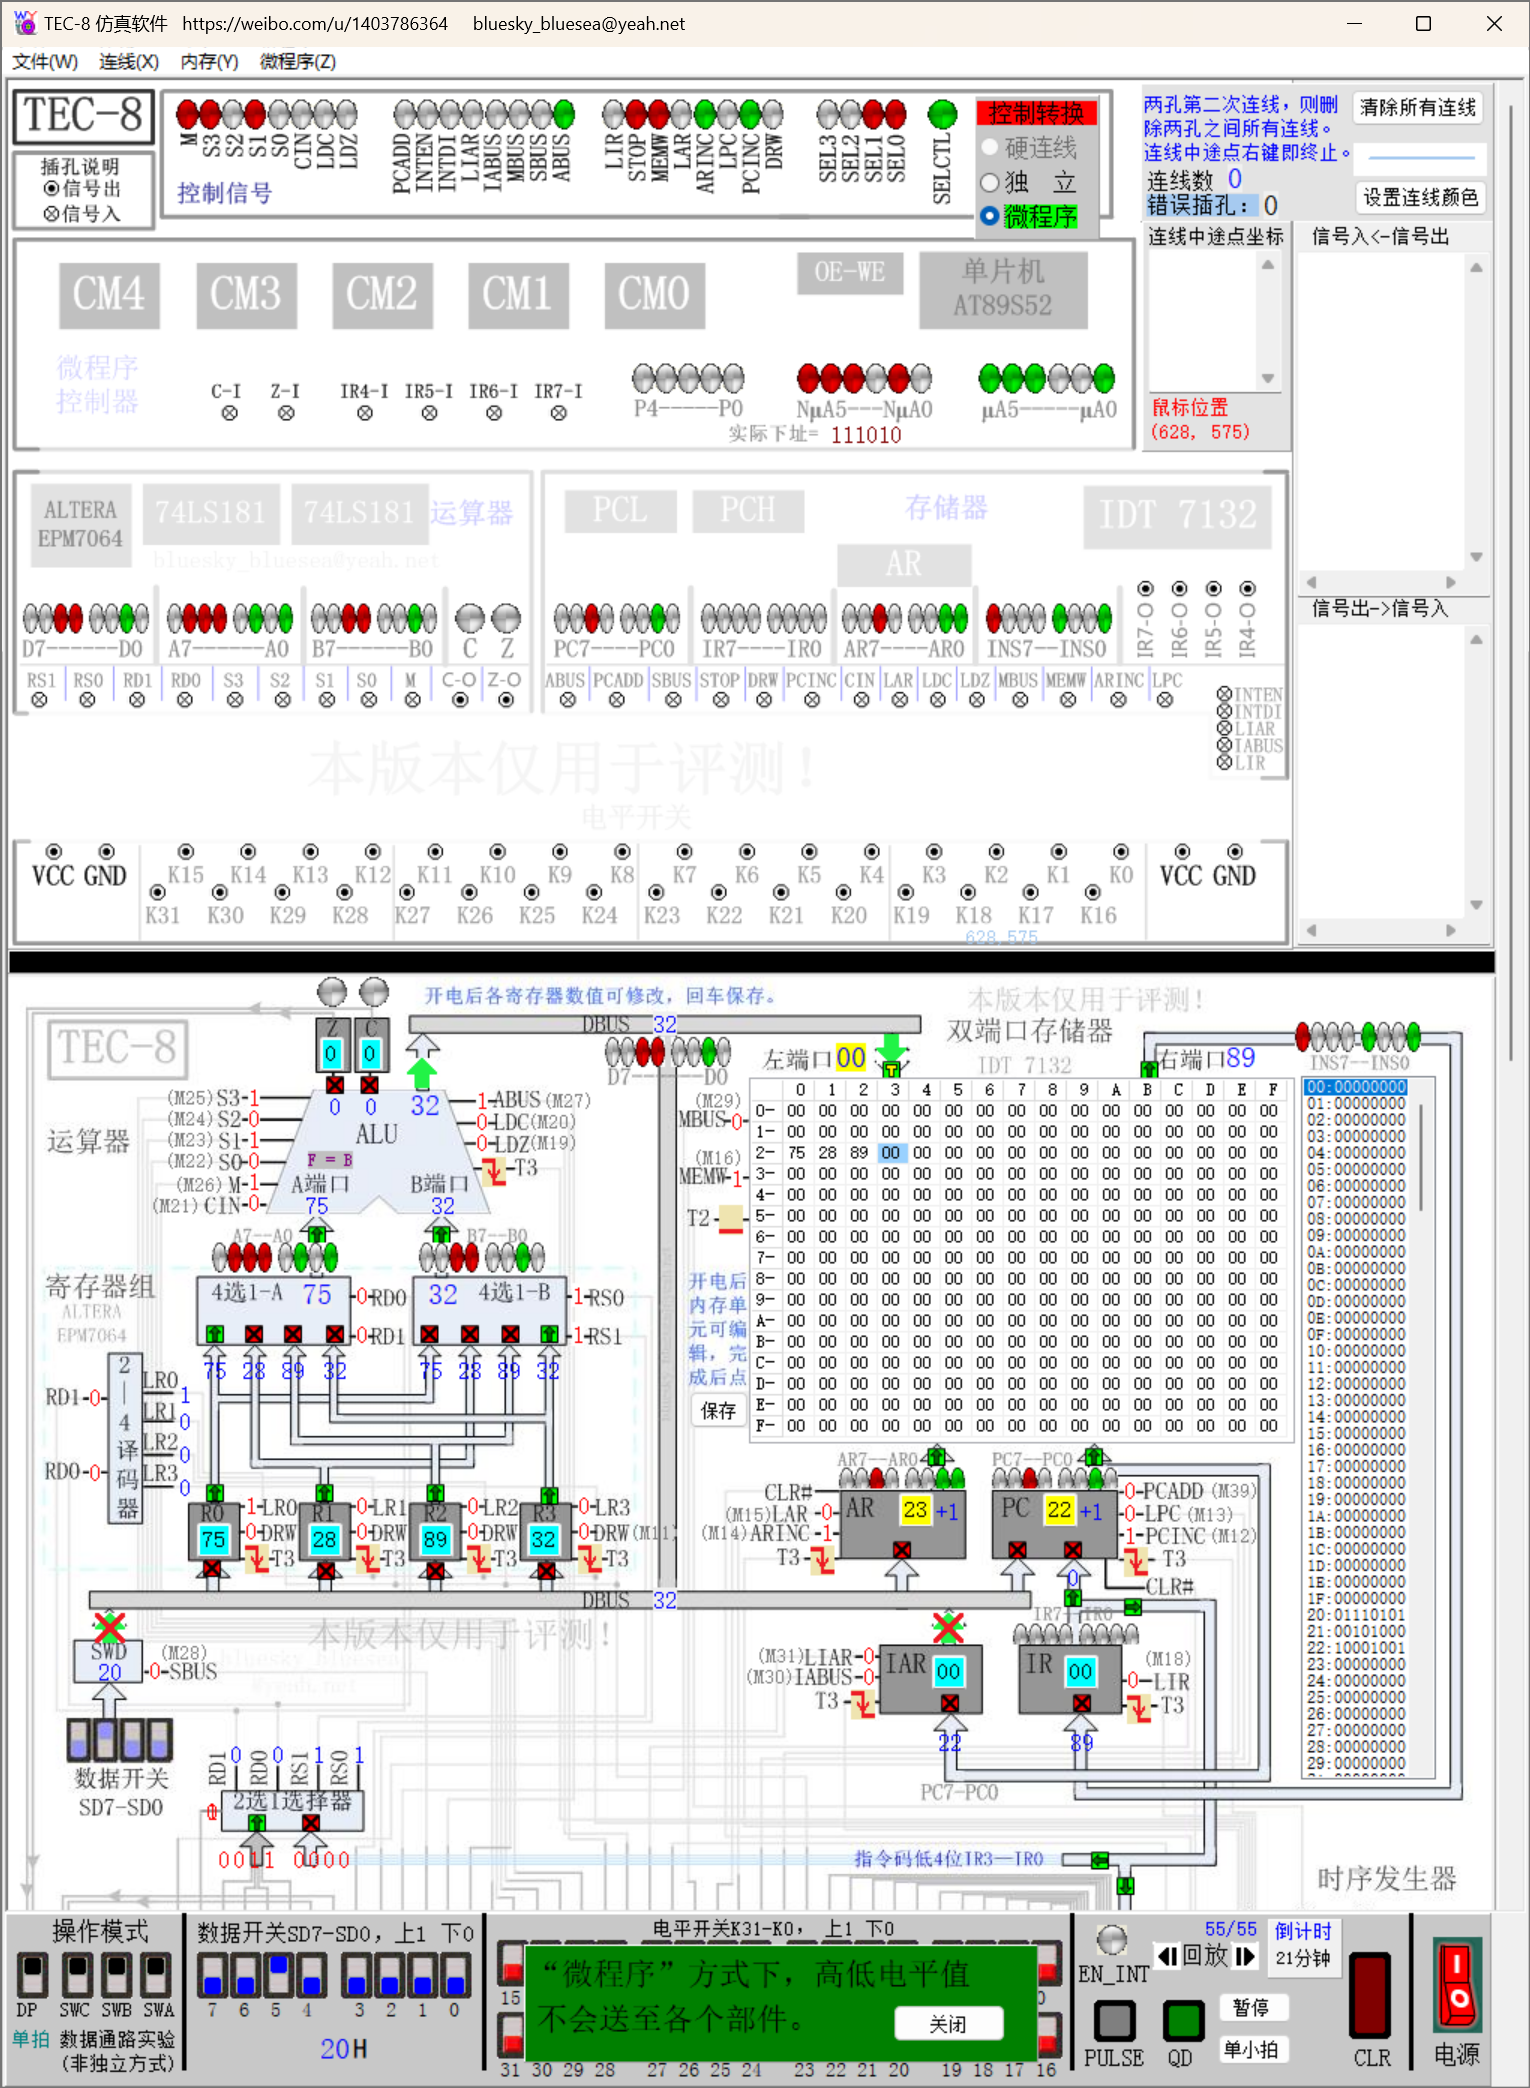
\includegraphics[width=0.3\textwidth]{screenshots/3.1.8.png}
              }
              \subfigure[将R$_3$数值写入23H单元]{
                  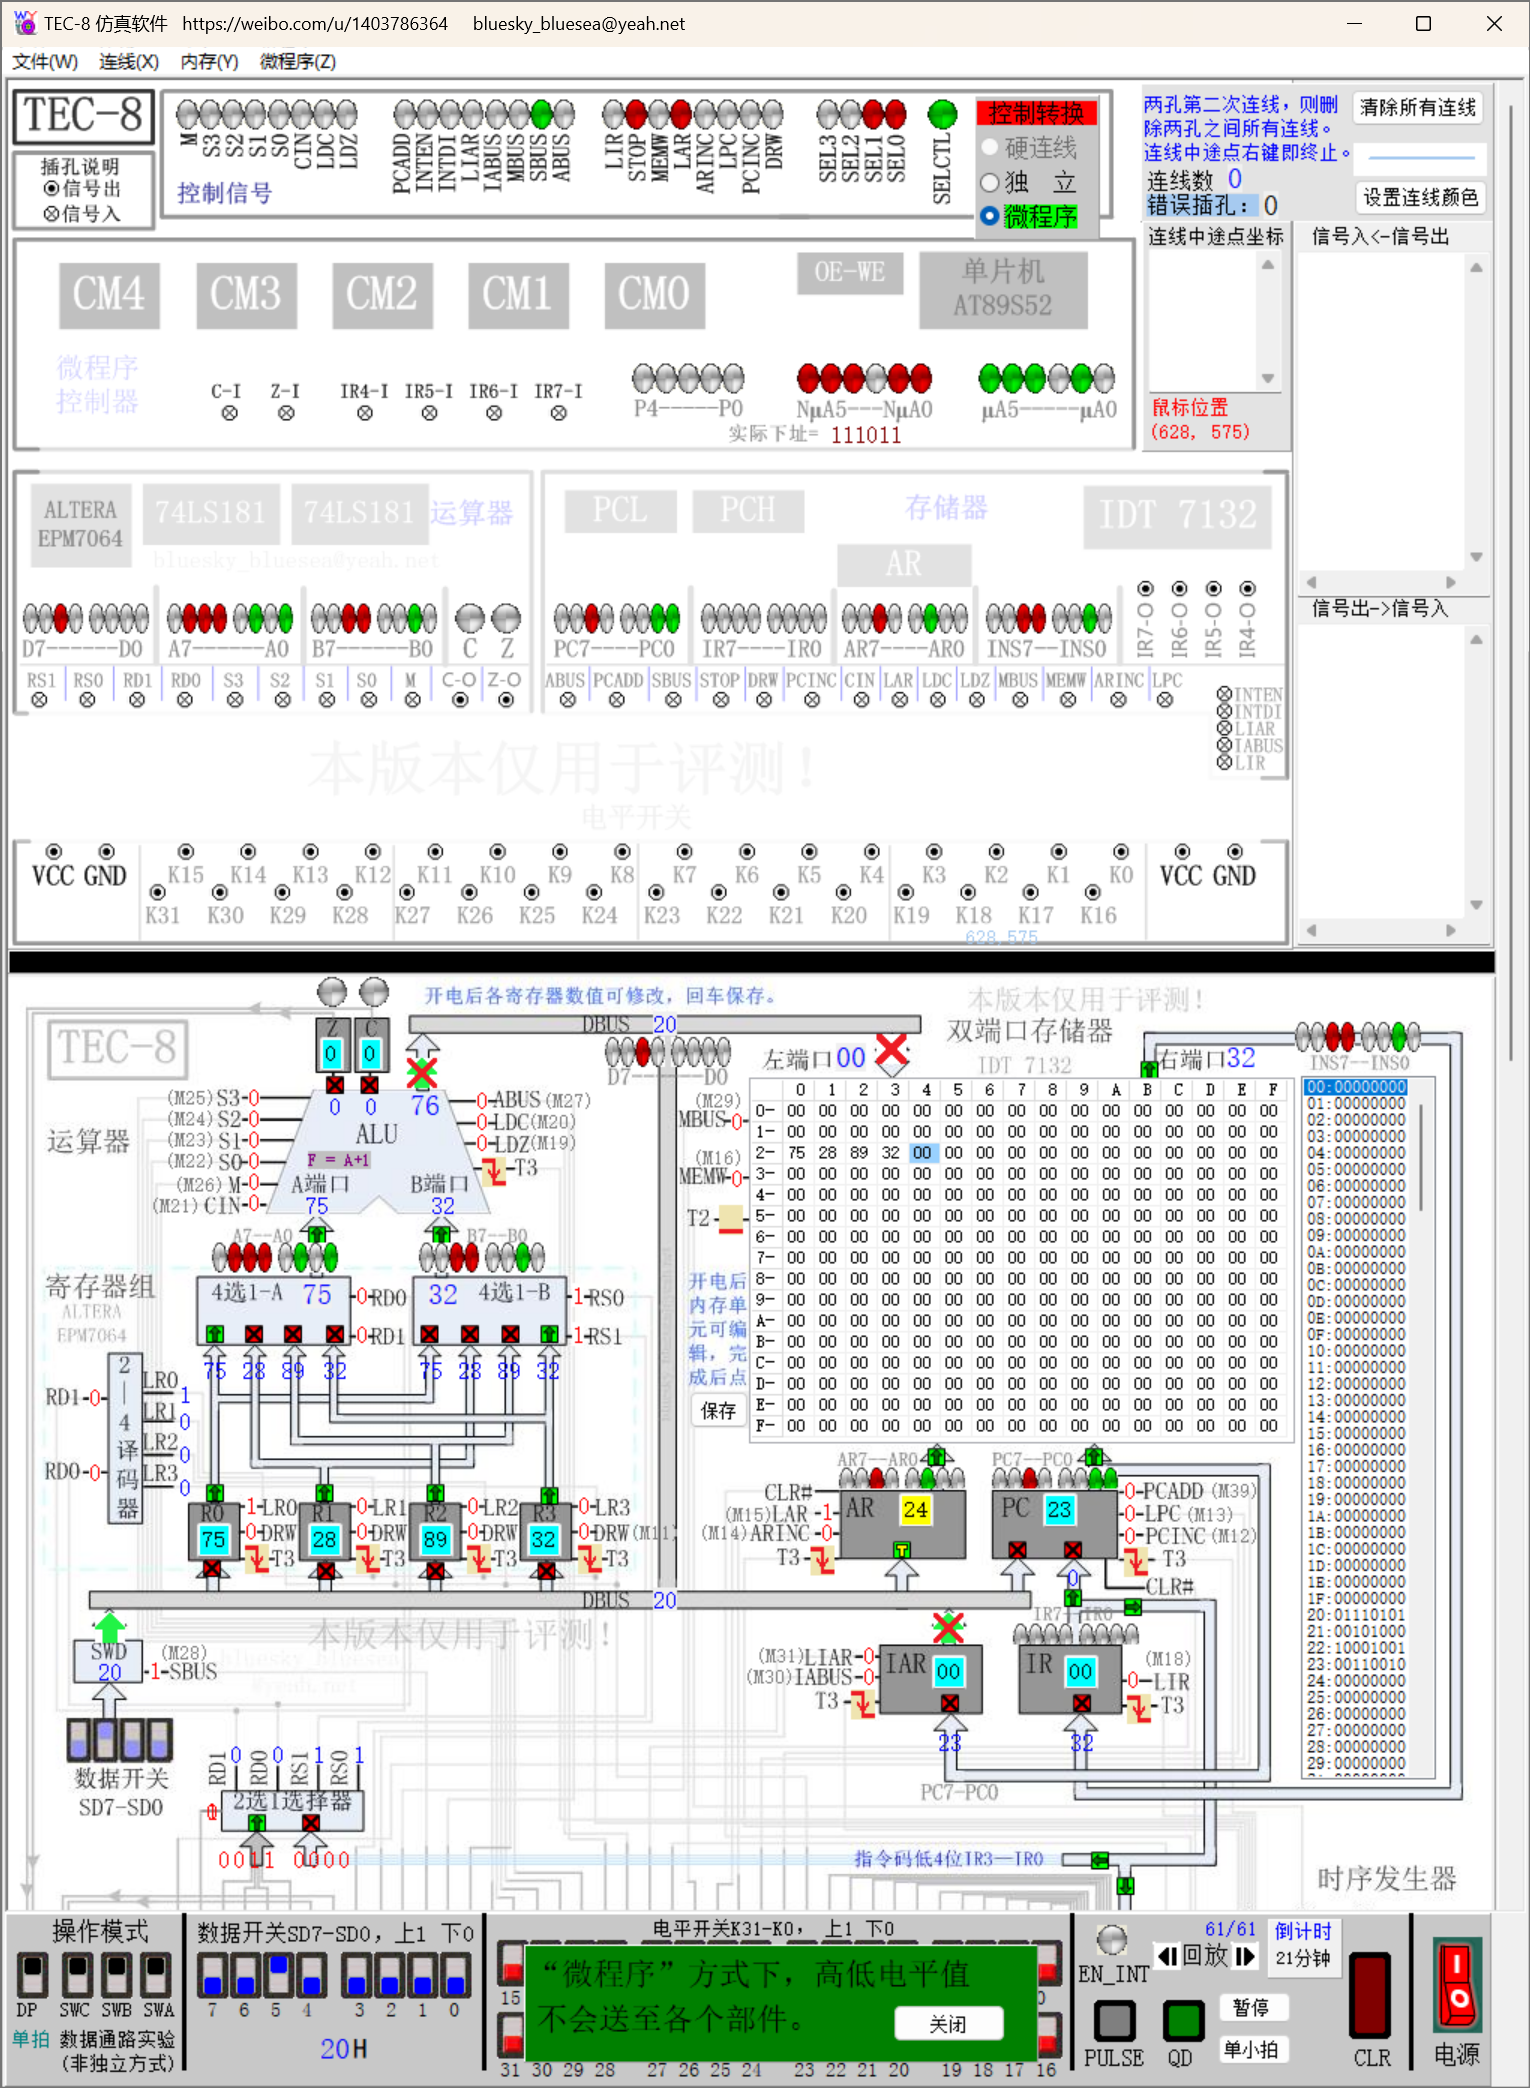
\includegraphics[width=0.3\textwidth]{screenshots/3.1.9.png}
              }
              \caption{写入存储器 (微程序)}
              \label{fig:3.3}
          \end{figure}

    \item 重新设置存储器地址 AR 和程序计数器 PC 为 20H. (如图 \ref{fig:3.4} 所示.)

          \begin{figure}[htbp]
              \centering
              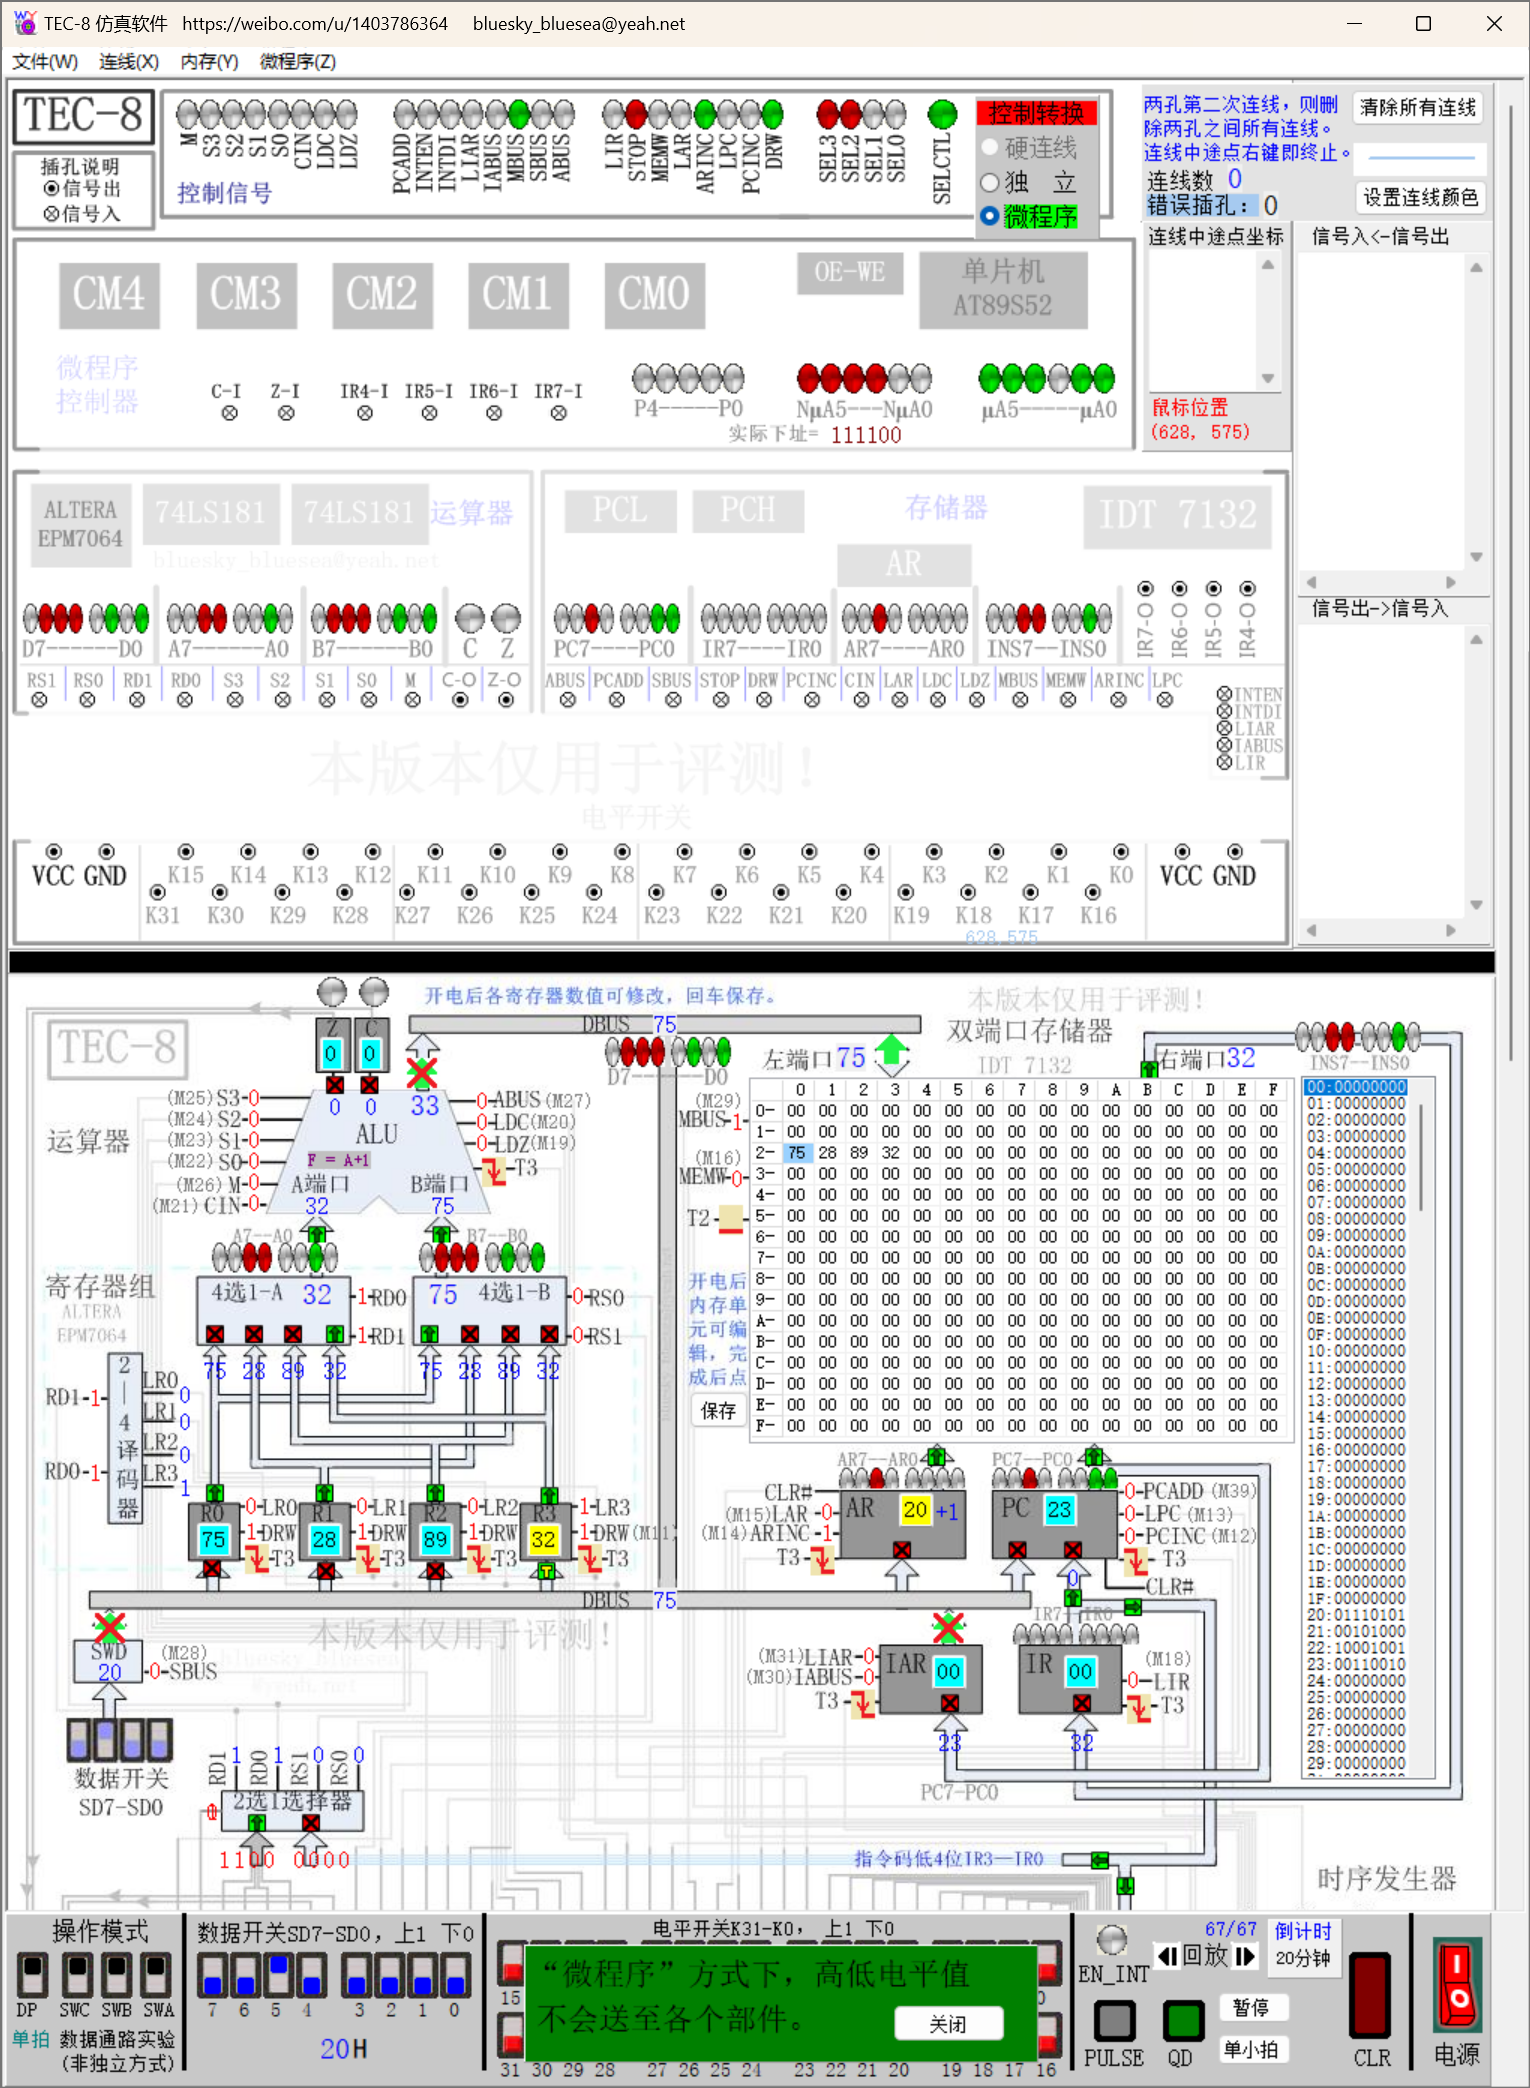
\includegraphics[width=0.3\textwidth]{screenshots/3.1.10.png}
              \caption{重设地址 (微程序)}
              \label{fig:3.4}
          \end{figure}

    \item 将存储器 20H、21H、22H 和 23H 单元中的数依次写入寄存器 R$_3$、R$_2$、R$_1$ 和 R$_0$. (如图 \ref{fig:3.5} 所示.)

          \begin{figure}[htbp]
              \centering
              \subfigure[将20H单元的数值写入R$_3$]{
                  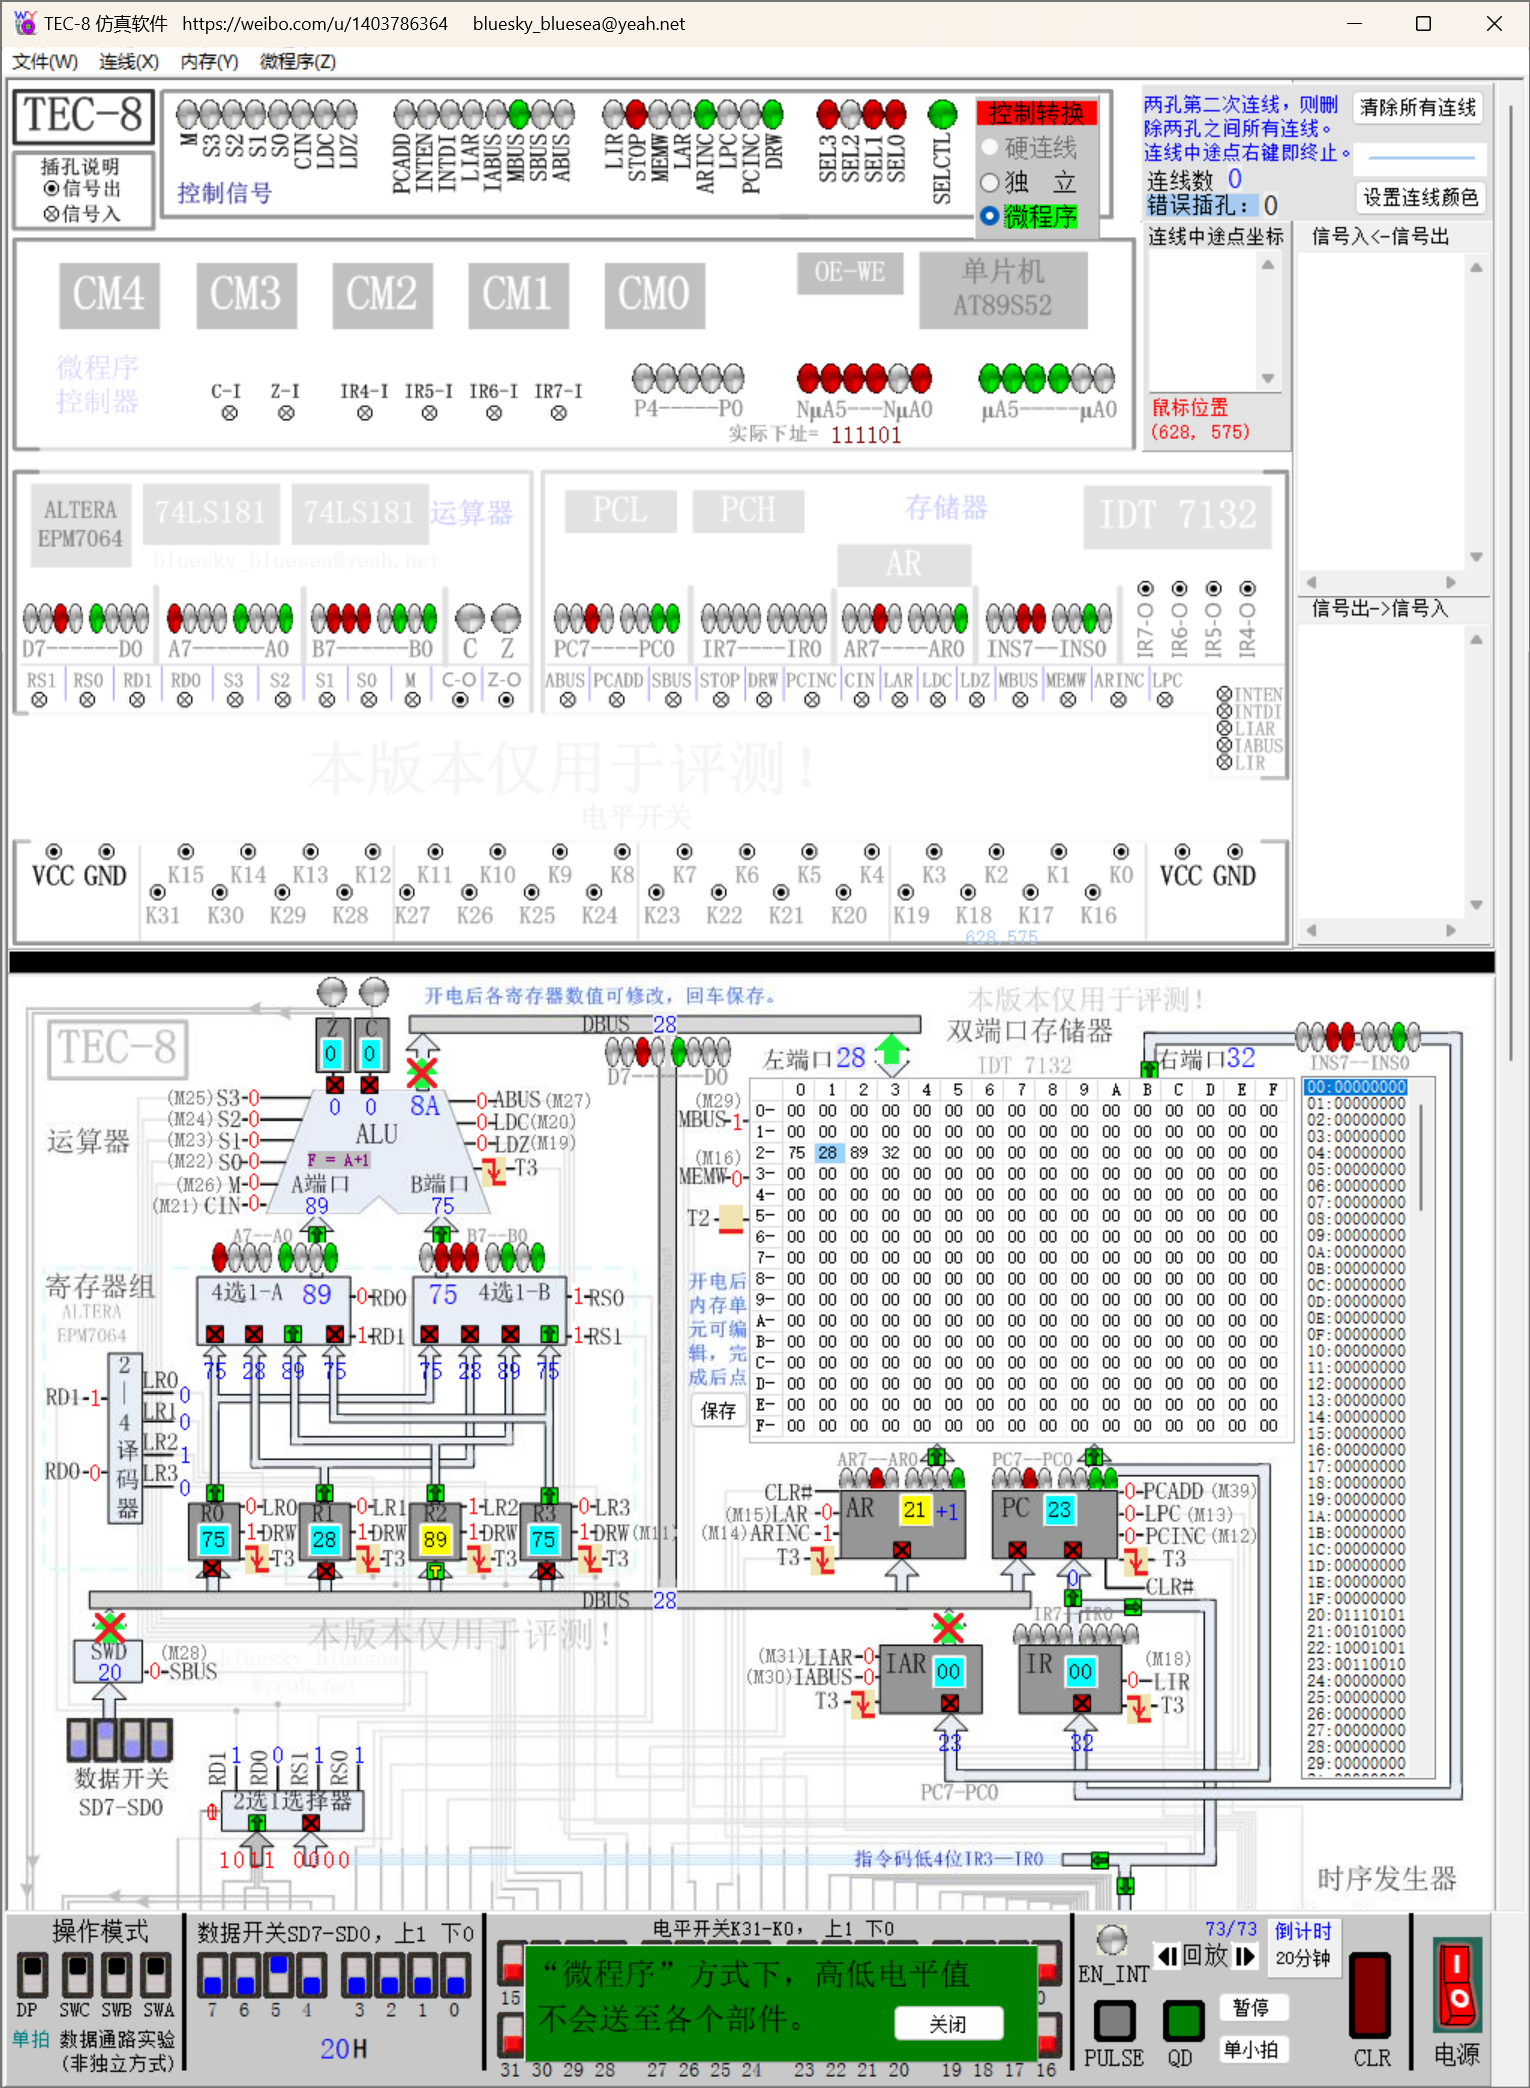
\includegraphics[width=0.3\textwidth]{screenshots/3.1.11.png}
              }
              \subfigure[将21H单元的数值写入R$_2$]{
                  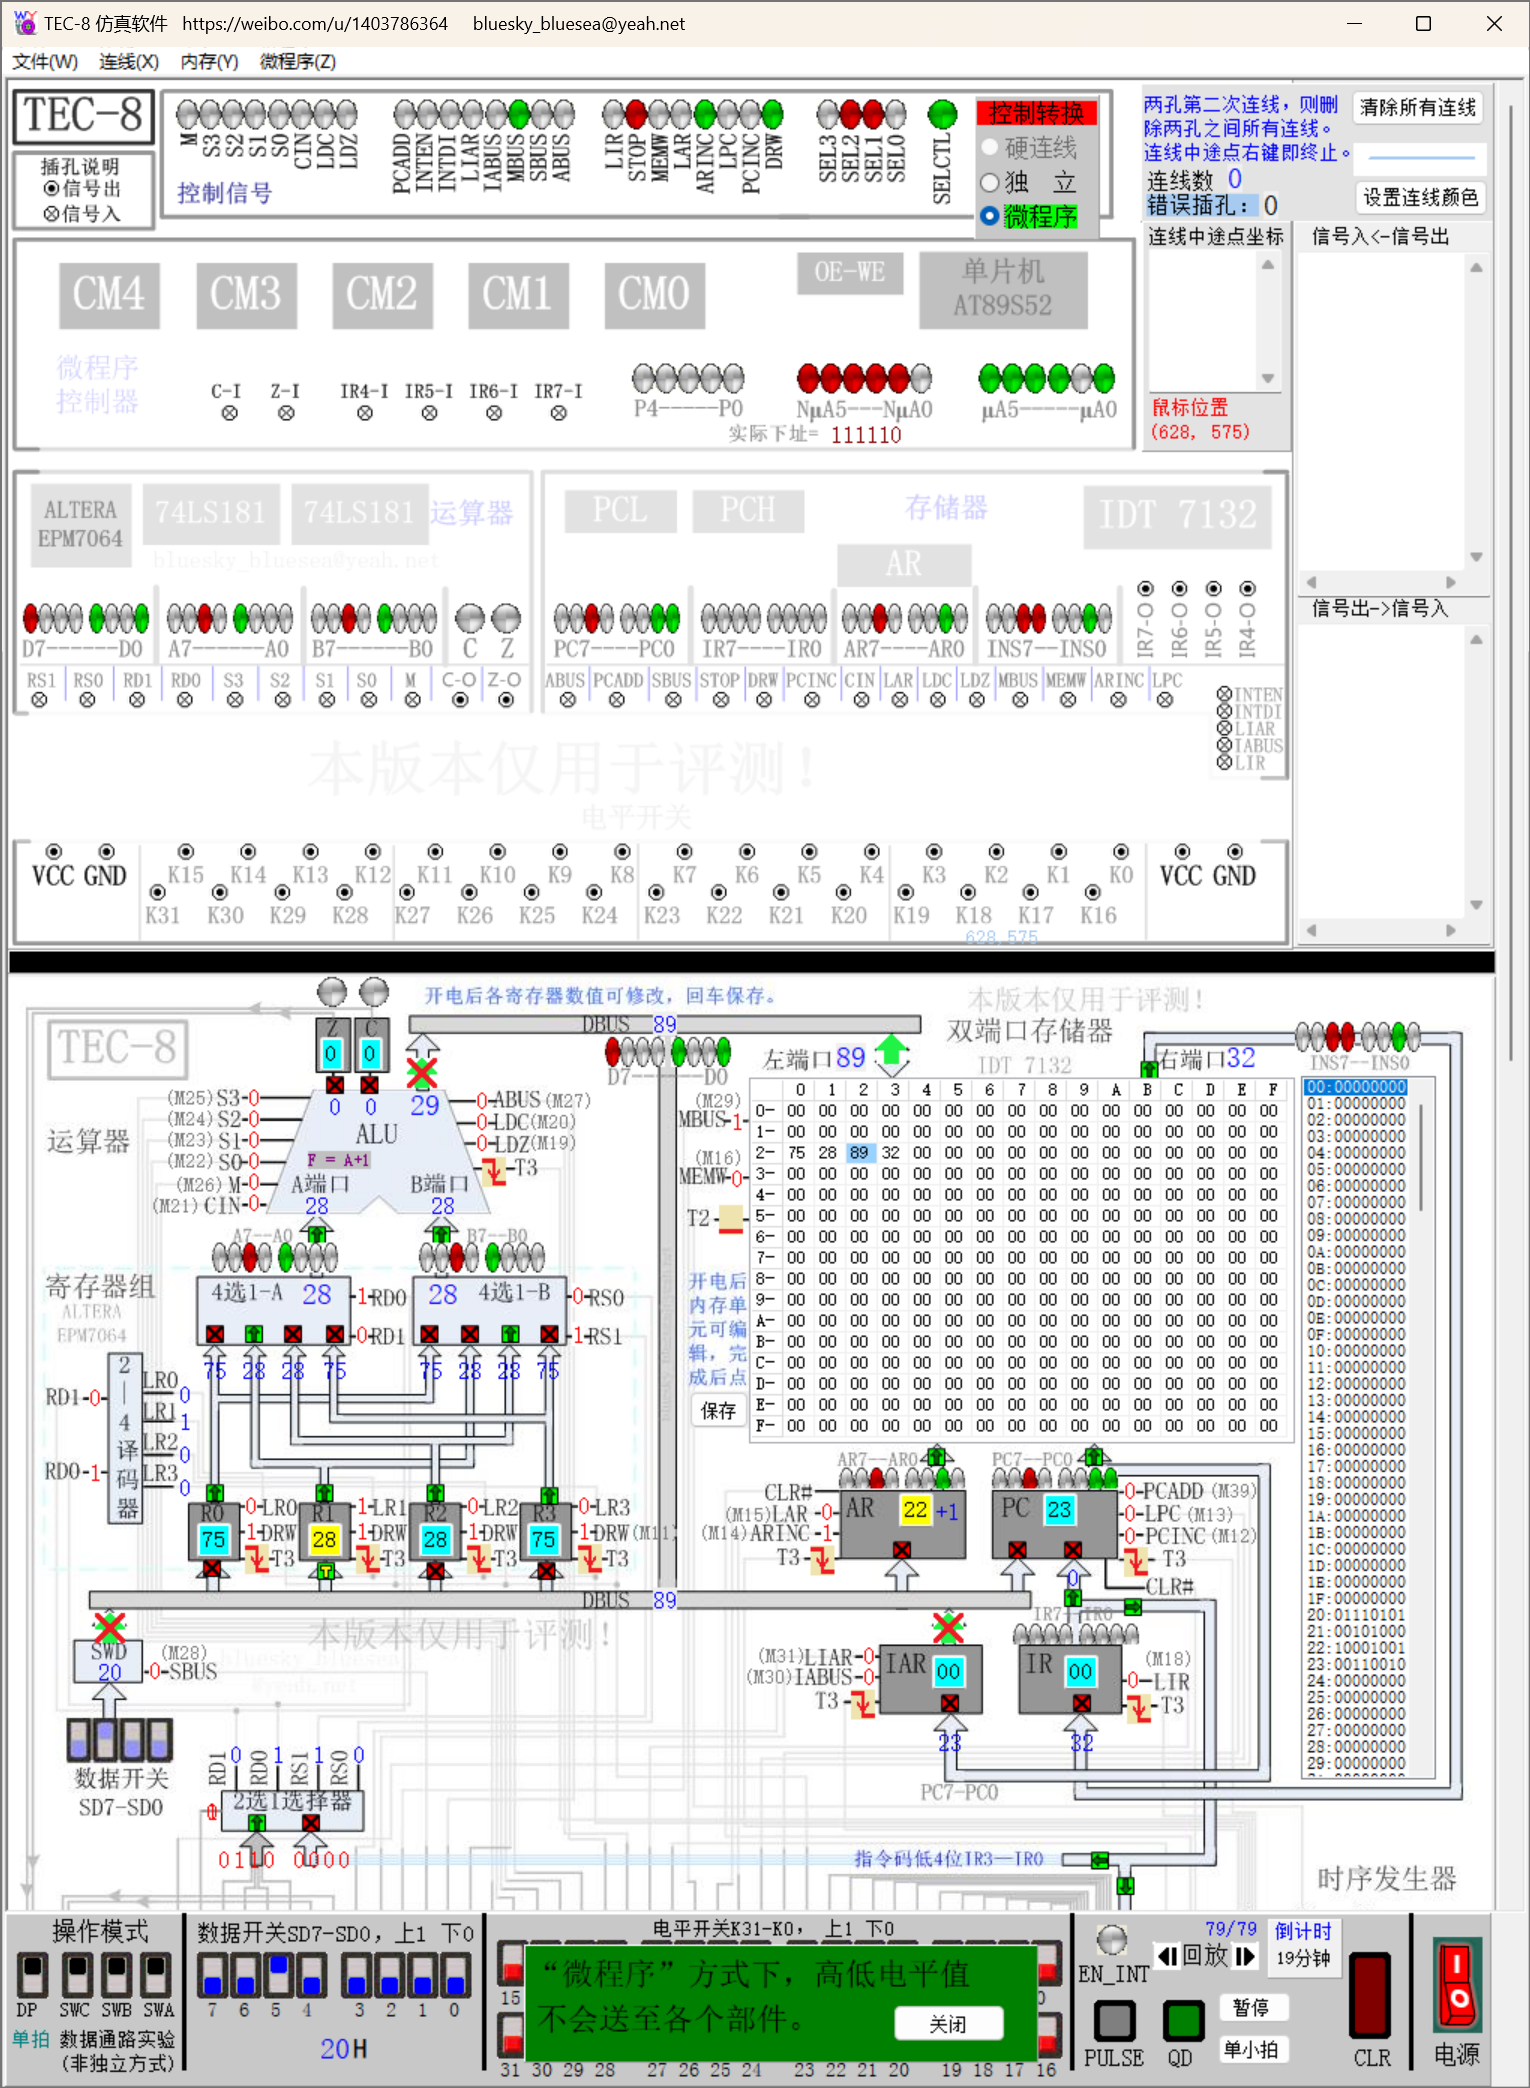
\includegraphics[width=0.3\textwidth]{screenshots/3.1.12.png}
              }
              \\
              \subfigure[将22H单元的数值写入R$_1$]{
                  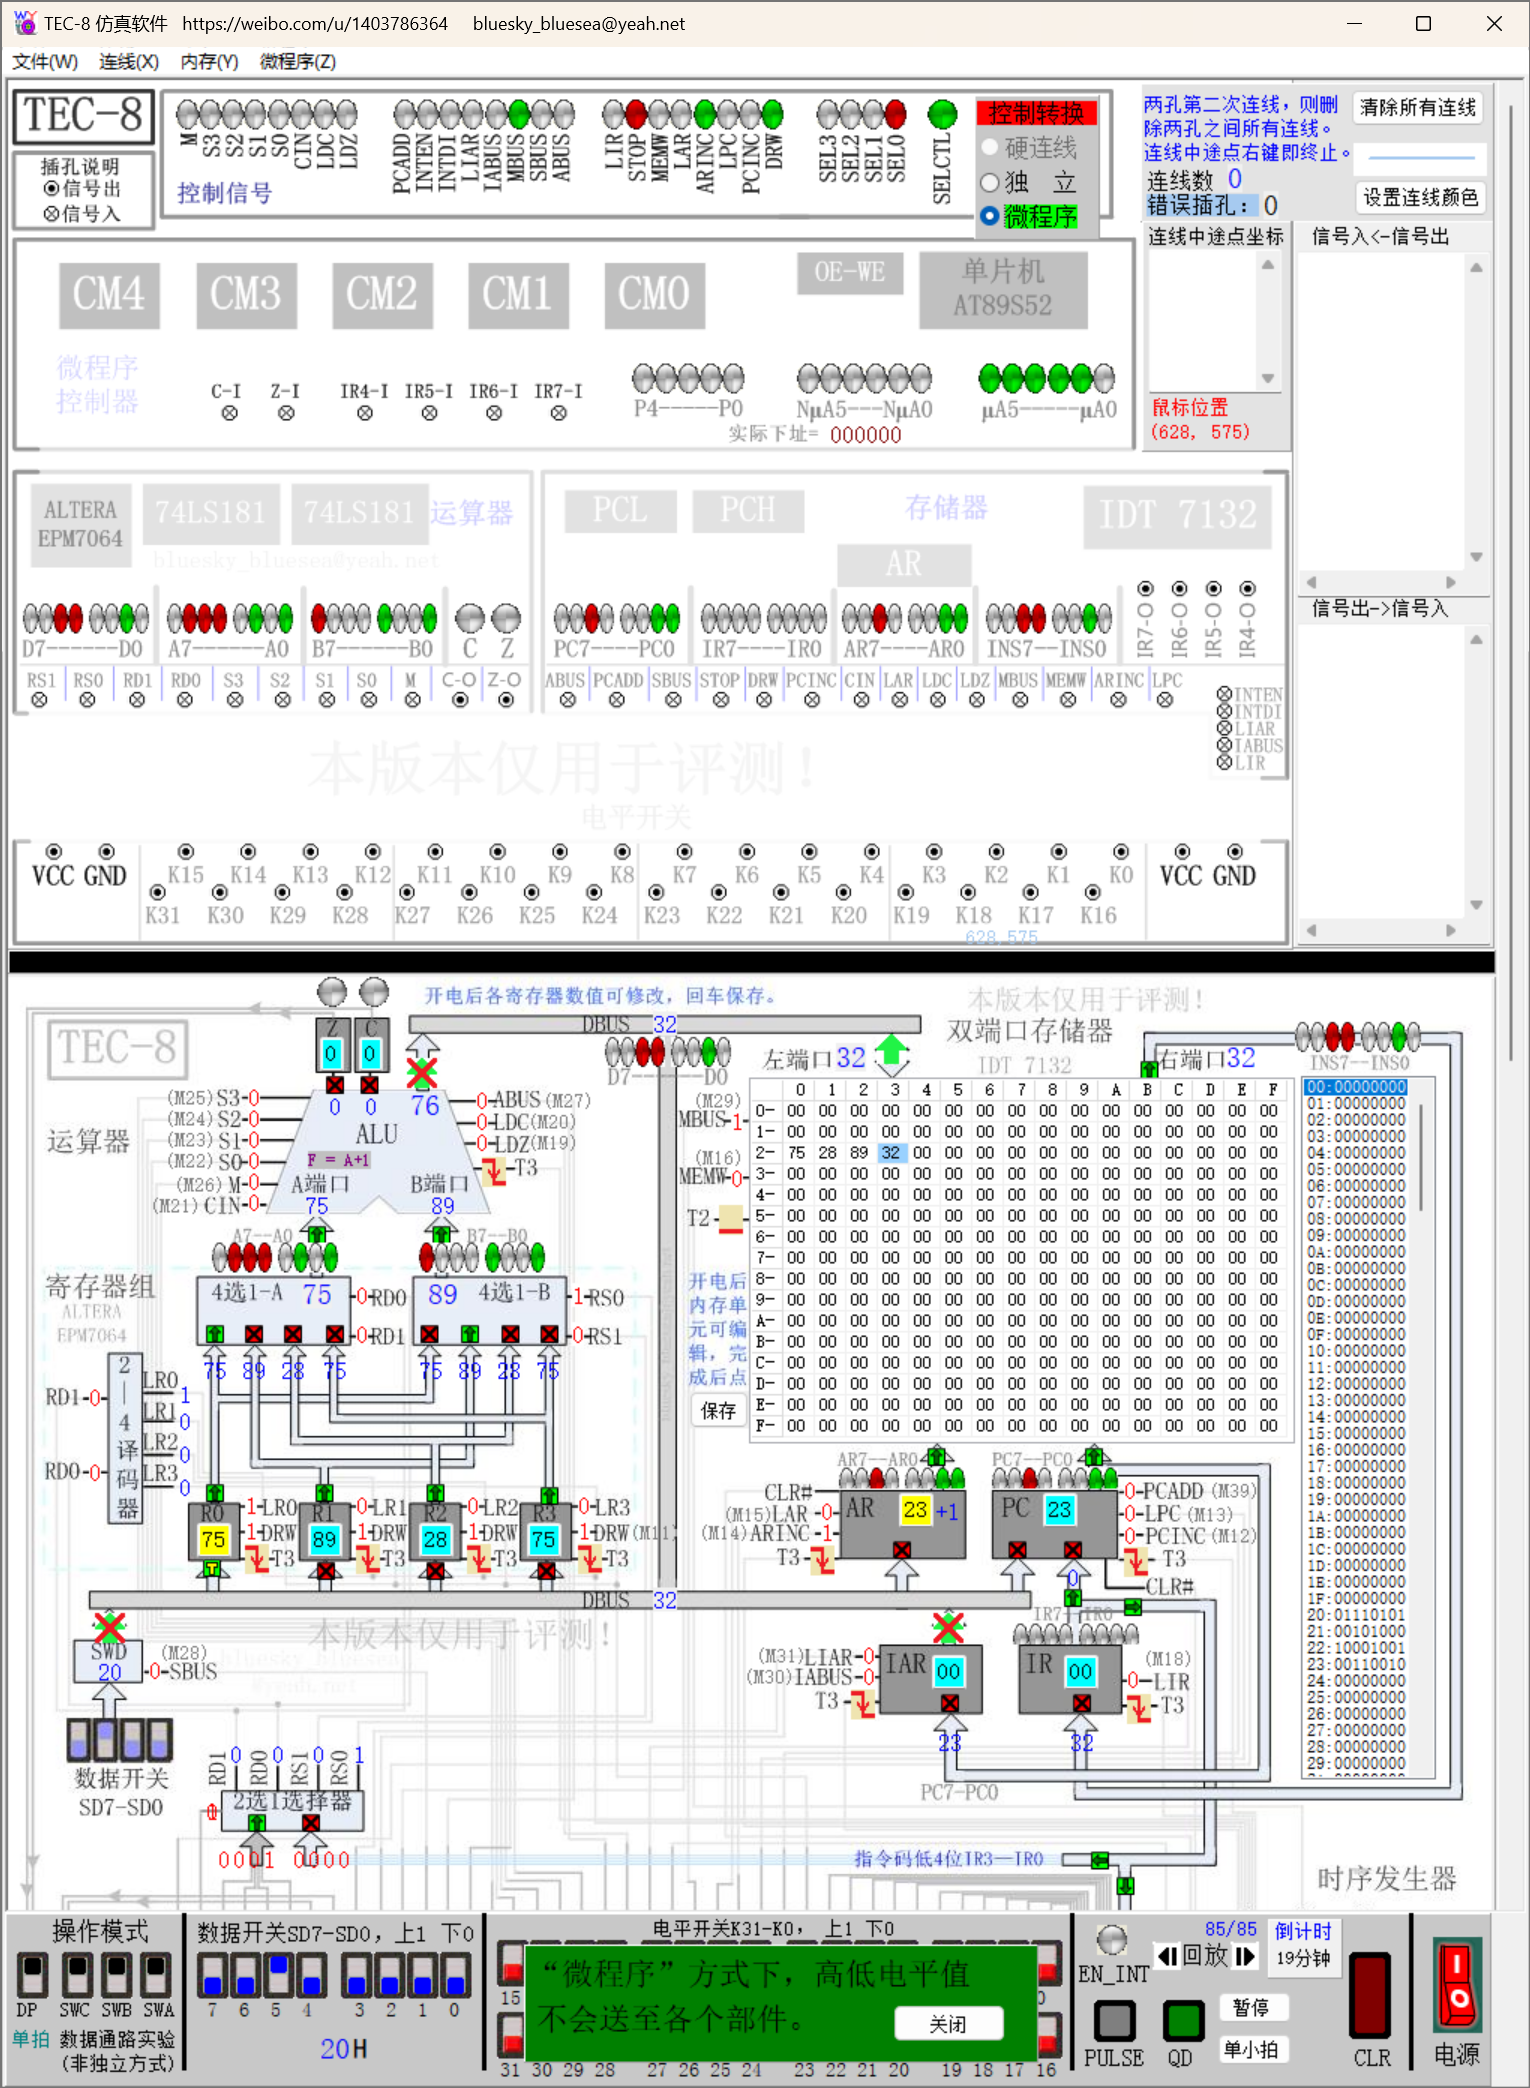
\includegraphics[width=0.3\textwidth]{screenshots/3.1.13.png}
              }
              \subfigure[将23H单元的数值写入R$_0$]{
                  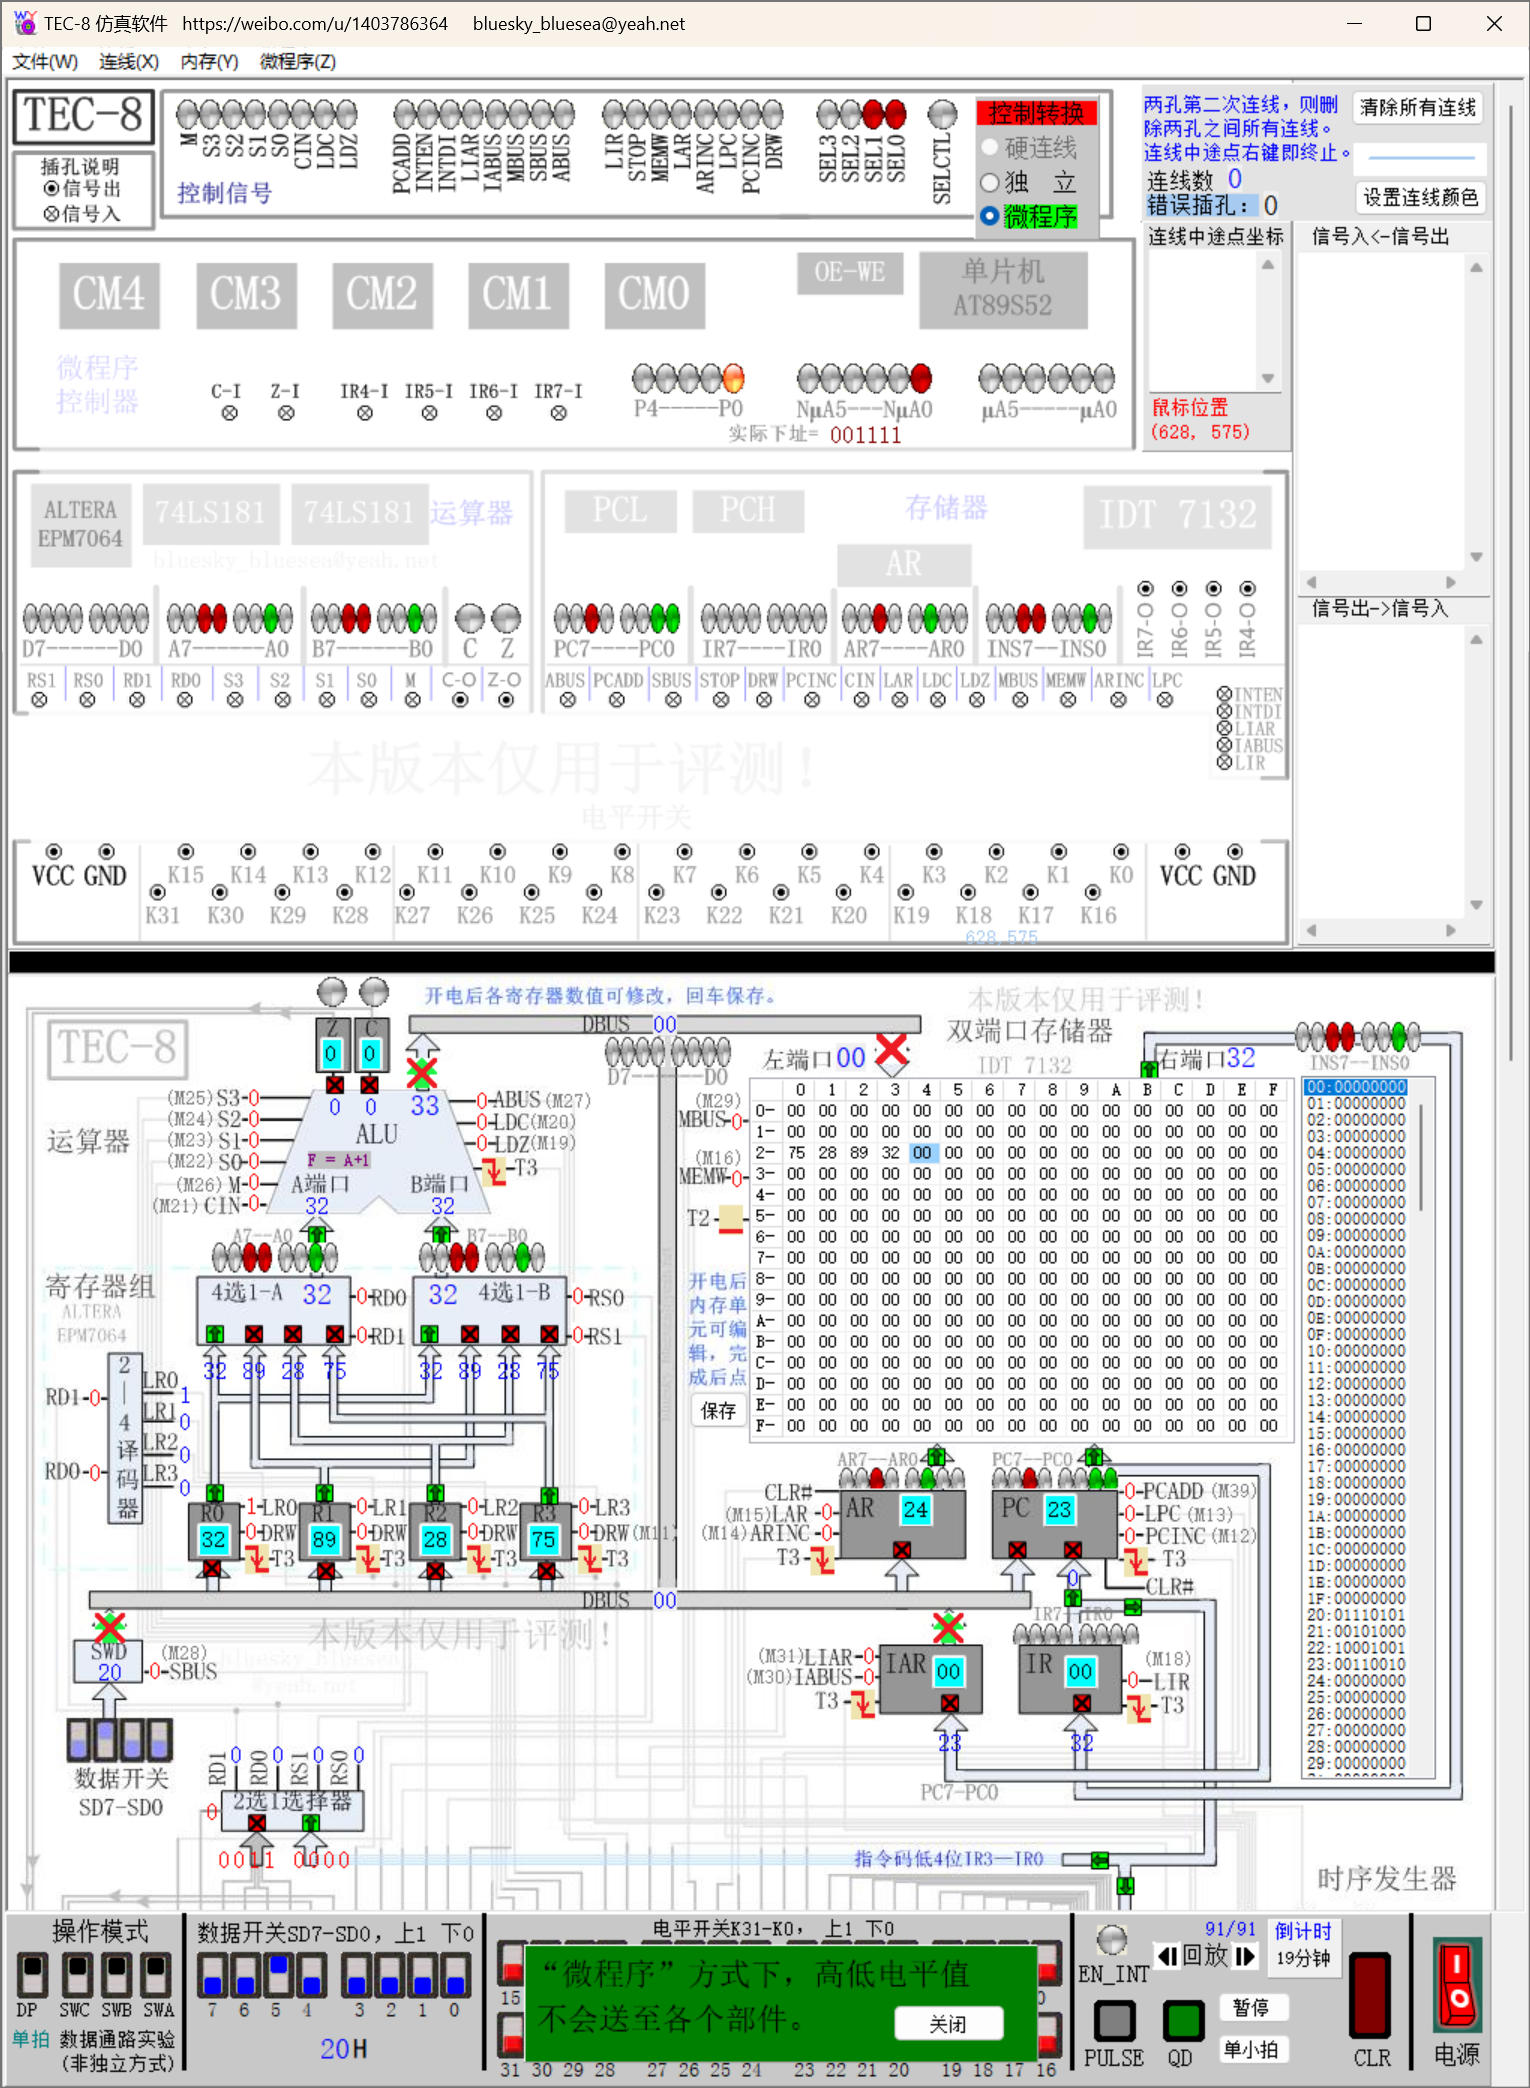
\includegraphics[width=0.3\textwidth]{screenshots/3.1.14.png}
              }
              \caption{写入寄存器 (微程序)}
              \label{fig:3.5}
          \end{figure}

    \item 实验结果如表 \ref{tab:3.1} 所示.

          \begin{table}[h]
              \centering
              \begin{tabular}{ccccccccccc}
                  \Xhline{1pt}
                  $\mathrm{\mu_{A_{5}-A_{0}}}$ & A$_{7-0}$ & B$_{7-0}$ & D$_{7-0}$ & AR  & PC  & INS$_{7-0}$ & R$_0$ & R$_1$ & R$_2$ & R$_3$ \\ \hline
                  00H                          & 00H       & 00H       & 00H       & 00H & 00H & 00H         & 00H   & 00H   & 00H   & 00H   \\
                  32H                          & 00H       & 75H       & 75H       & 00H & 00H & 00H         & 75H   & 00H   & 00H   & 00H   \\
                  33H                          & 00H       & 28H       & 28H       & 00H & 00H & 00H         & 75H   & 28H   & 00H   & 00H   \\
                  34H                          & 00H       & 89H       & 89H       & 00H & 00H & 00H         & 75H   & 28H   & 89H   & 00H   \\
                  35H                          & 75H       & 32H       & 32H       & 00H & 00H & 00H         & 75H   & 28H   & 89H   & 32H   \\
                  36H                          & 75H       & 75H       & 75H       & 20H & 20H & 00H         & 75H   & 28H   & 89H   & 32H   \\
                  37H                          & 75H       & 28H       & 28H       & 21H & 20H & 75H         & 75H   & 28H   & 89H   & 32H   \\
                  38H                          & 75H       & 89H       & 89H       & 22H & 21H & 28H         & 75H   & 28H   & 89H   & 32H   \\
                  39H                          & 75H       & 32H       & 32H       & 23H & 22H & 89H         & 75H   & 28H   & 89H   & 32H   \\
                  3AH                          & 75H       & 32H       & 20H       & 24H & 23H & 32H         & 75H   & 28H   & 89H   & 32H   \\
                  3BH                          & 32H       & 75H       & 75H       & 20H & 23H & 32H         & 75H   & 28H   & 89H   & 32H   \\
                  3CH                          & 89H       & 75H       & 28H       & 21H & 23H & 32H         & 75H   & 28H   & 89H   & 75H   \\
                  3DH                          & 28H       & 28H       & 89H       & 22H & 23H & 32H         & 75H   & 28H   & 28H   & 75H   \\
                  3EH                          & 75H       & 89H       & 32H       & 23H & 23H & 32H         & 75H   & 89H   & 28H   & 75H   \\
                  00H                          & 32H       & 32H       & 00H       & 24H & 23H & 32H         & 32H   & 89H   & 28H   & 75H   \\ \Xhline{1pt}
              \end{tabular}
              \caption{数据通路实验结果表}
              \label{tab:3.1}
          \end{table}

\end{enumerate}

\subsection{独立模式}

\begin{enumerate}

    \item 完成实验相关连线, 打开电源, 准备进入数据通路实验. (如图 \ref{fig:3.6} 所示.)

          \begin{figure}[htbp]
              \centering
              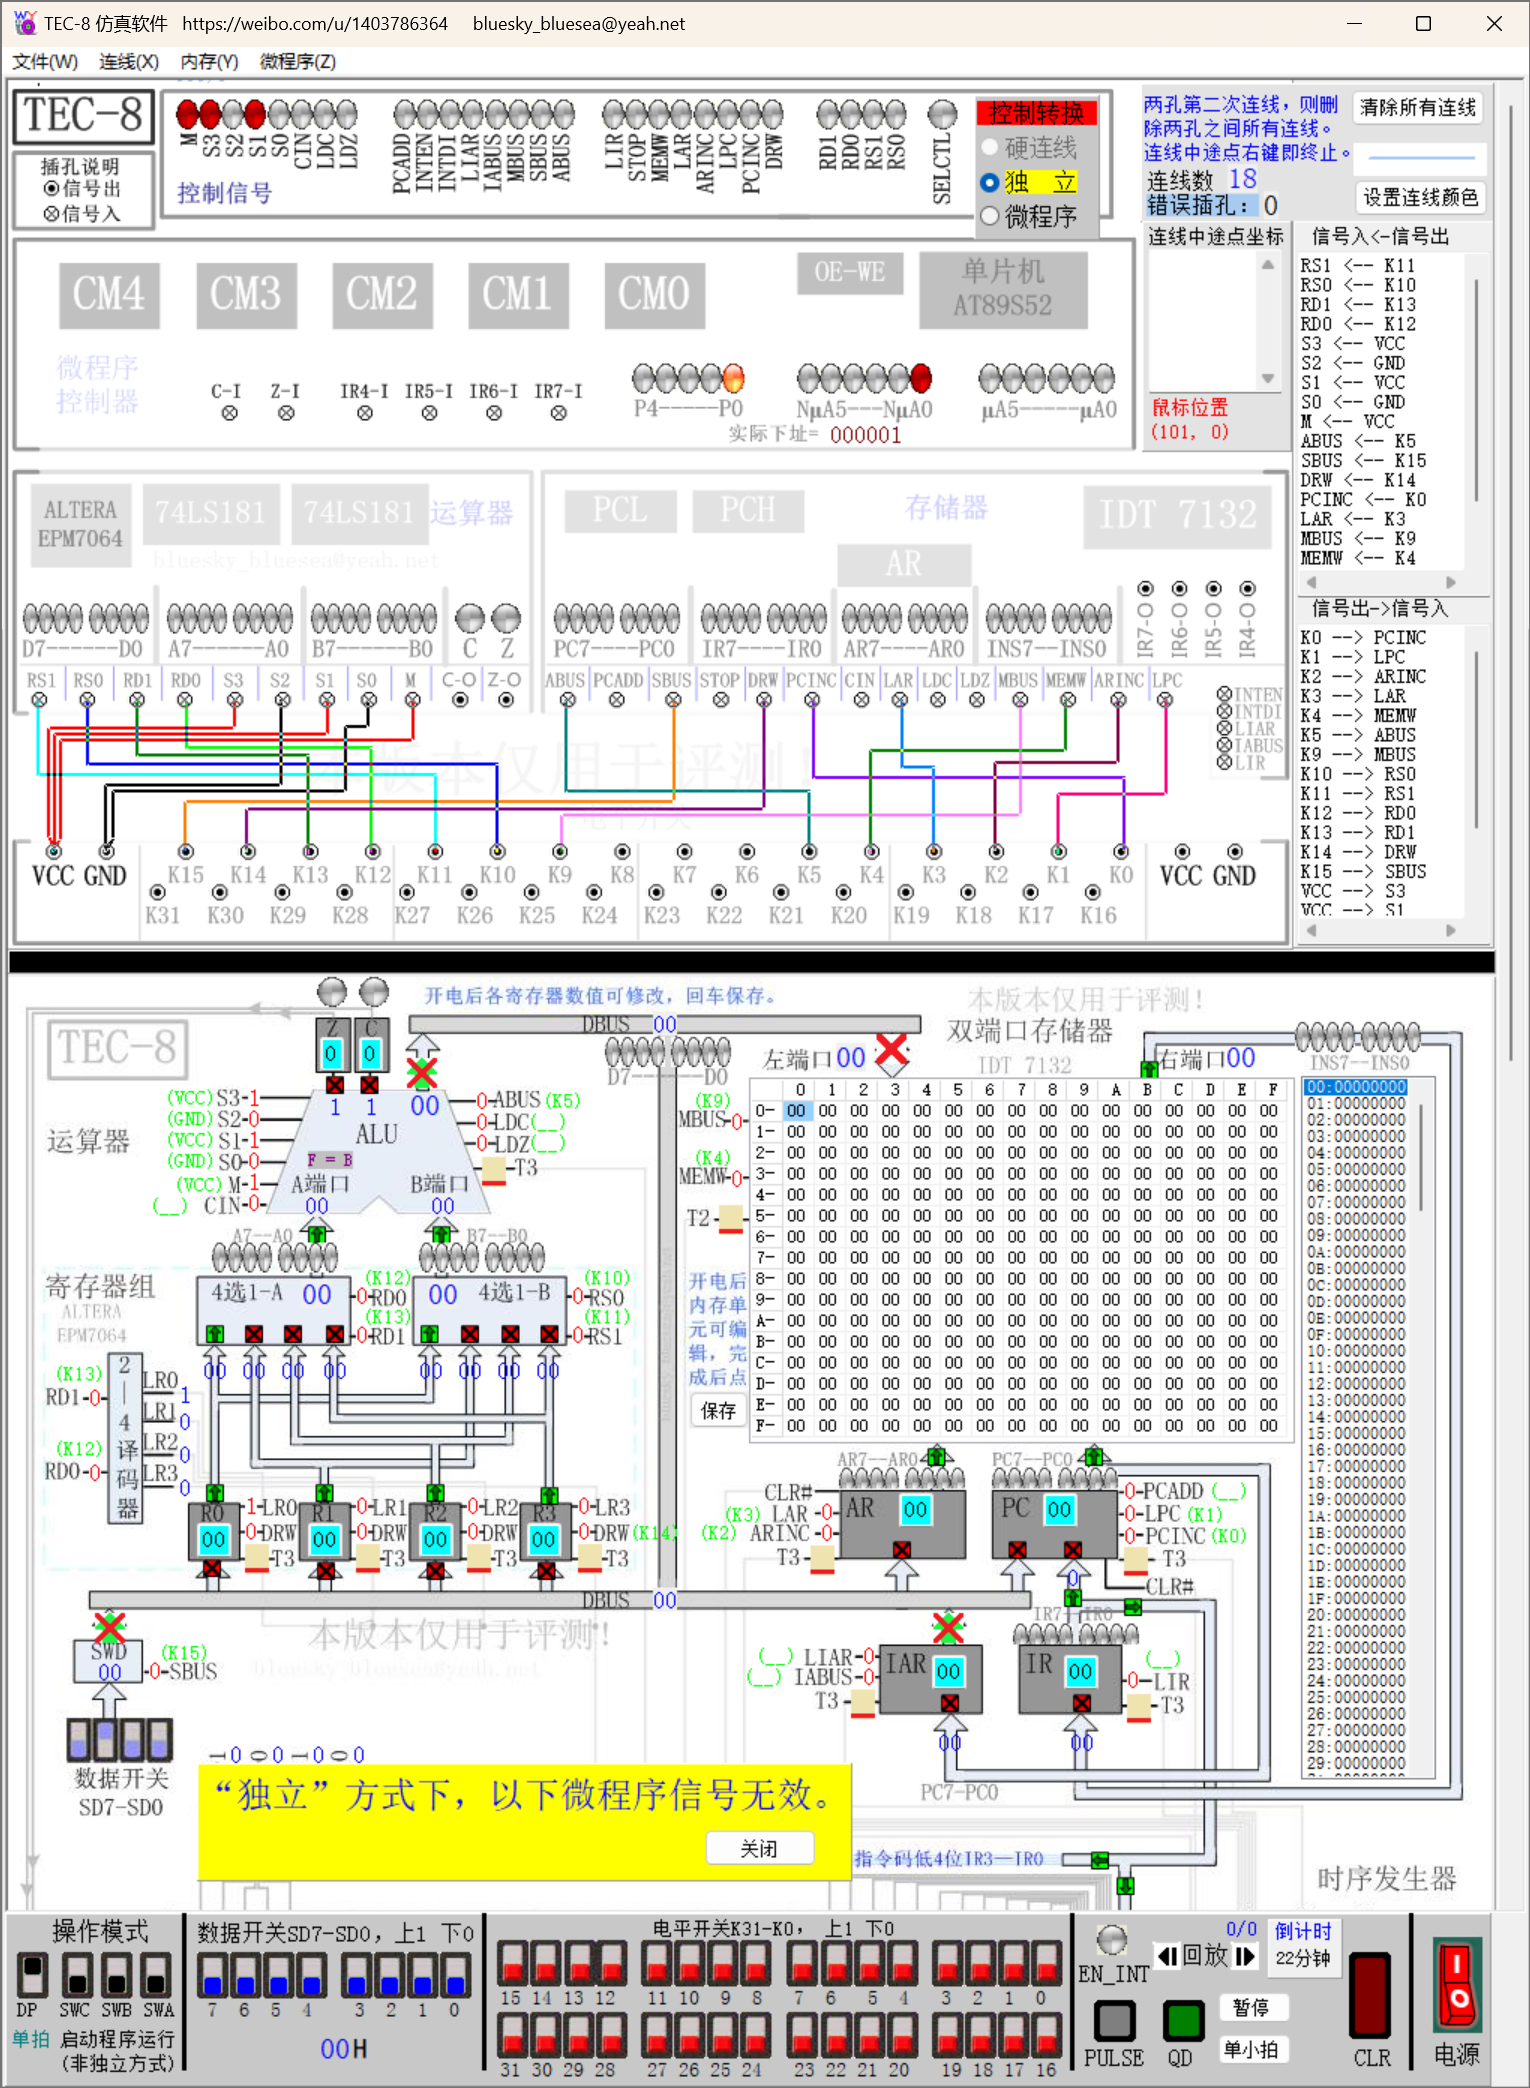
\includegraphics[width=0.3\textwidth]{screenshots/3.2.1.png}
              \caption{实验连线 (独立)}
              \label{fig:3.6}
          \end{figure}

    \item 通过数据开关依次将数 75H 写到寄存器 R$_0$, 数 28H 写到 R$_1$, 数 89H 写到 R$_2$, 数 32H 写到 R$_3$. (如图 \ref{fig:3.7} 所示.)

          \begin{figure}[htbp]
              \centering
              \subfigure[将数 75H 写到 R$_0$]{
                  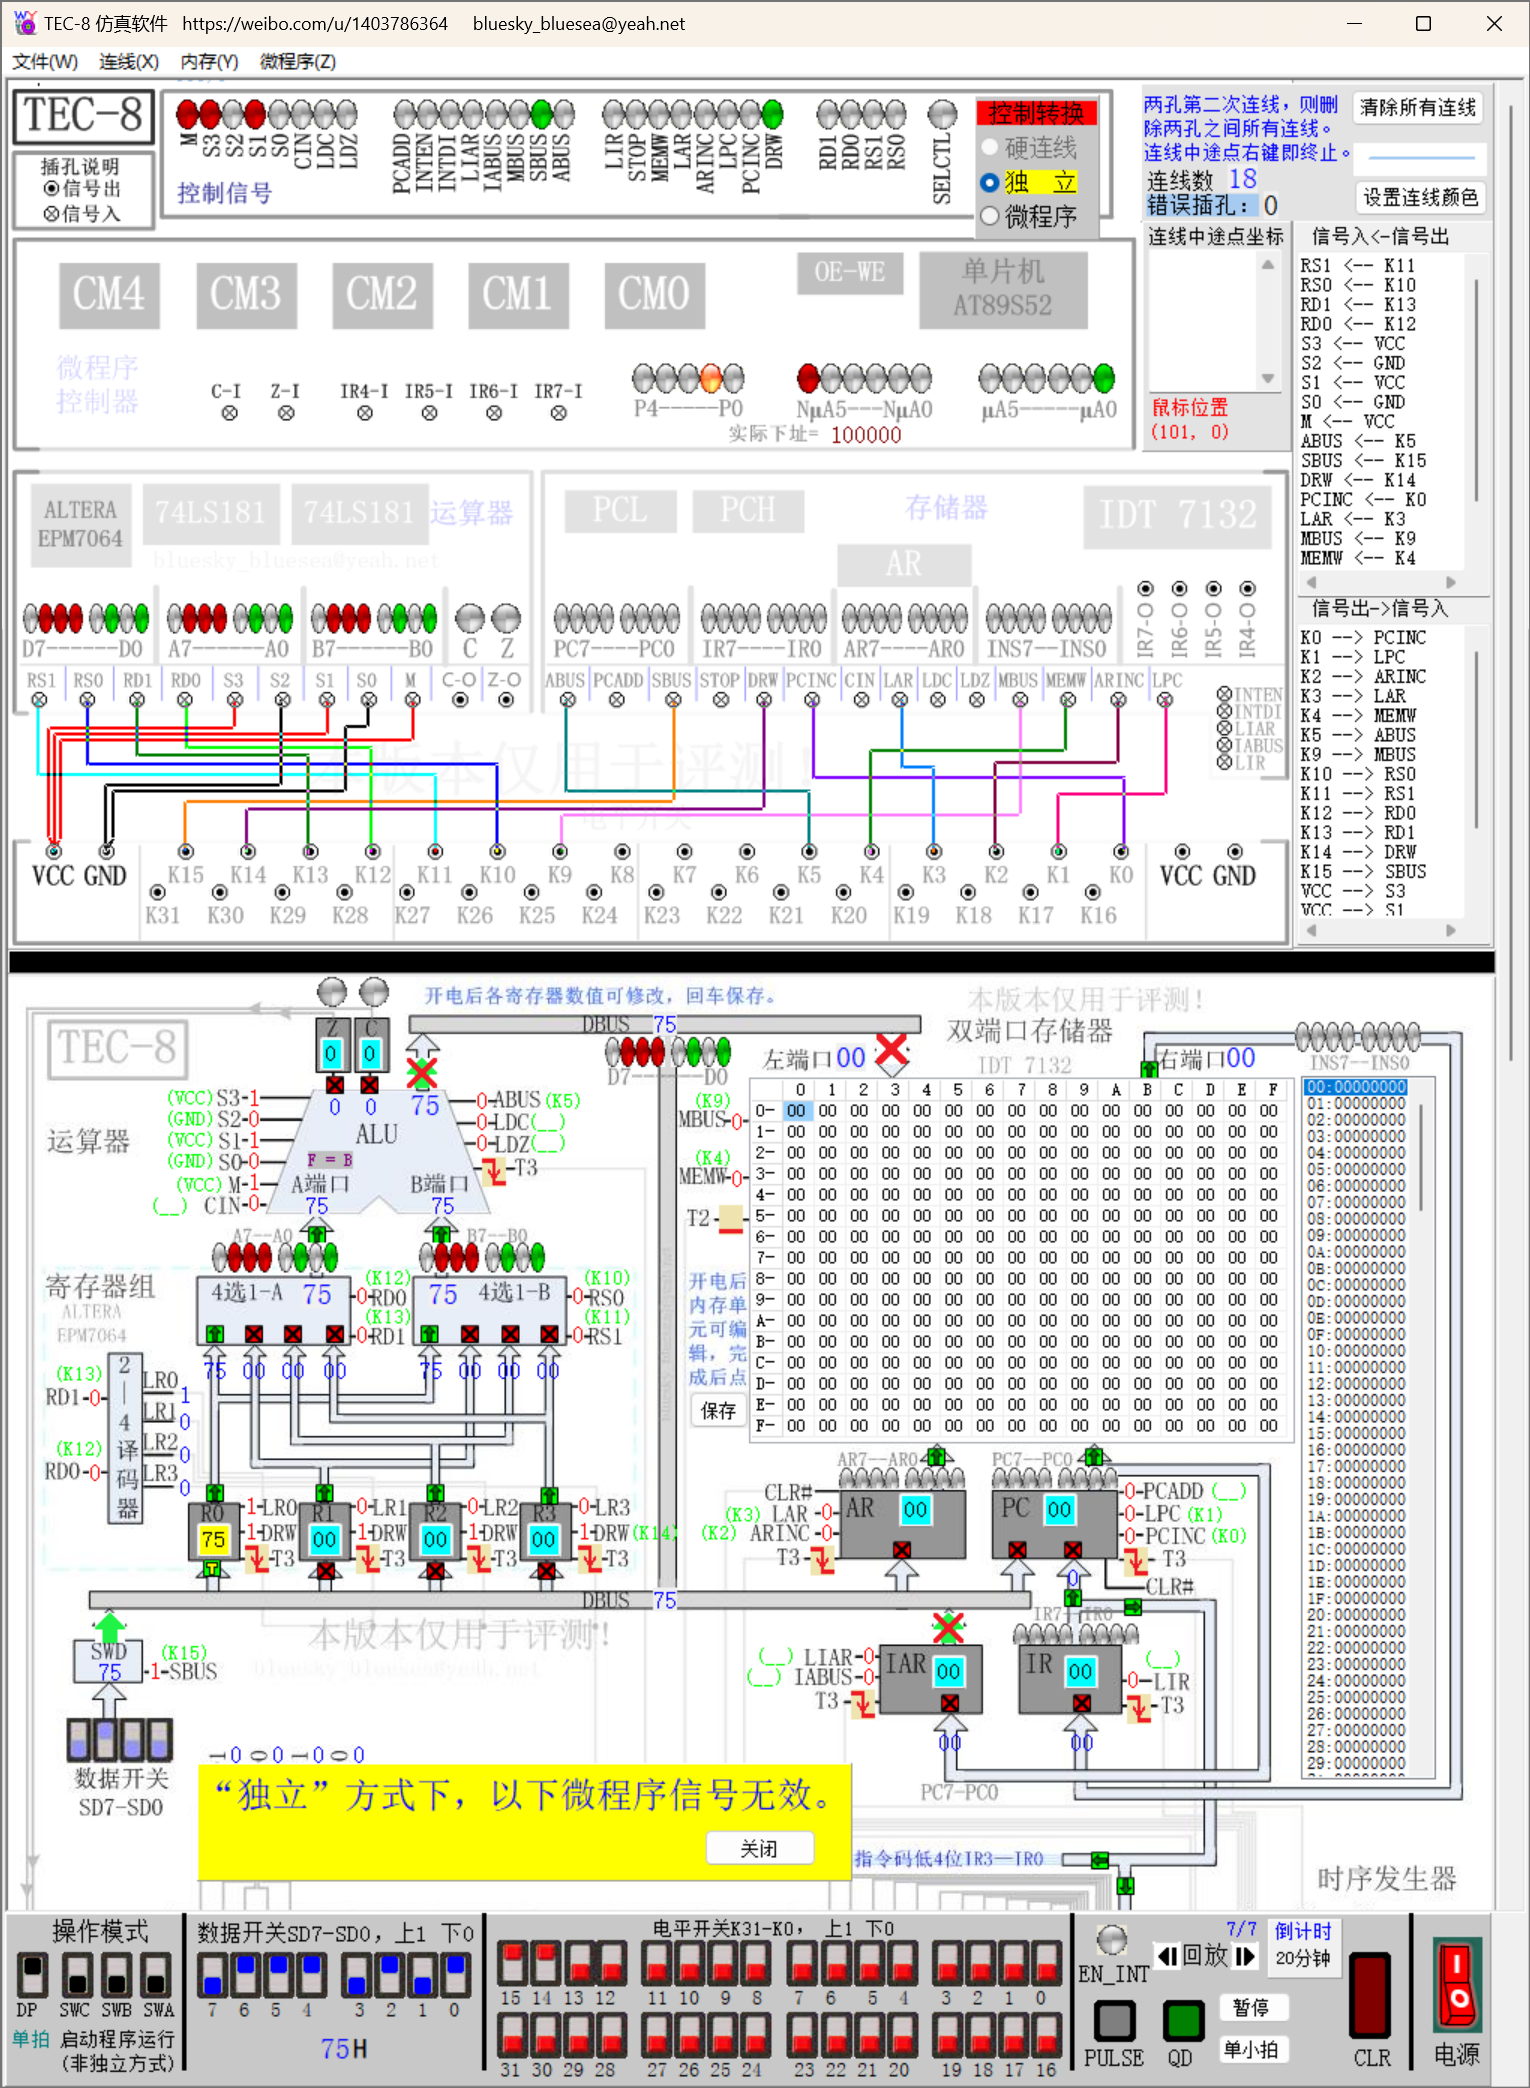
\includegraphics[width=0.3\textwidth]{screenshots/3.2.2.png}
              }
              \subfigure[将数 28H 写到 R$_1$]{
                  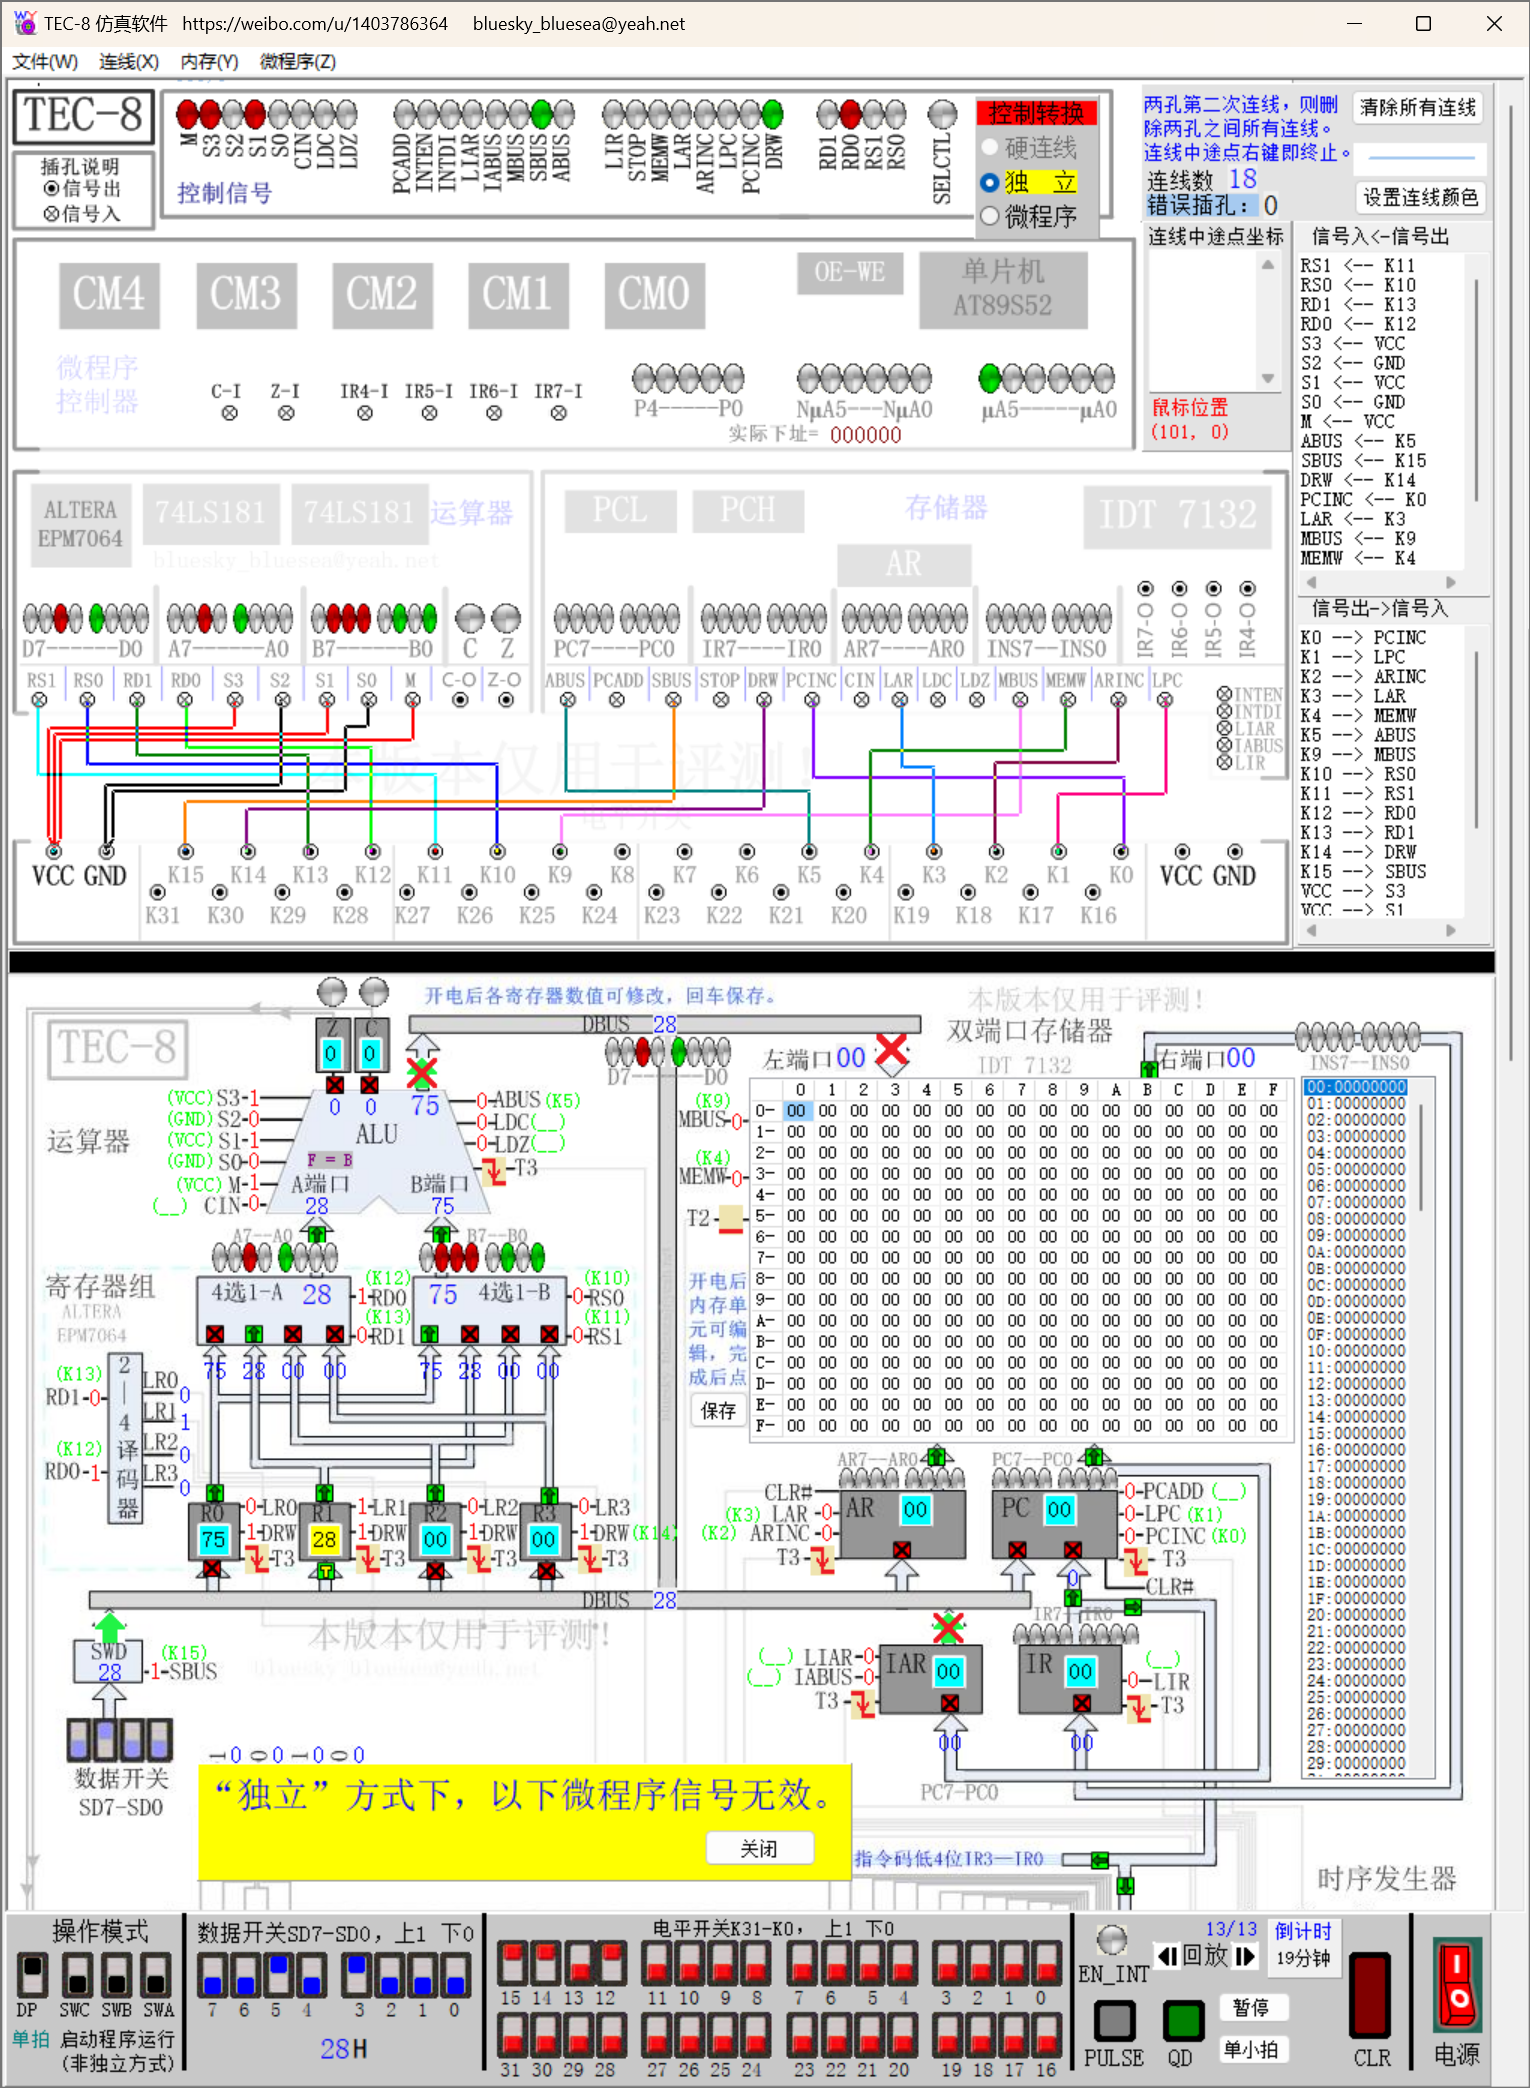
\includegraphics[width=0.3\textwidth]{screenshots/3.2.3.png}
              }
              \\
              \subfigure[将数 89H 写到 R$_2$]{
                  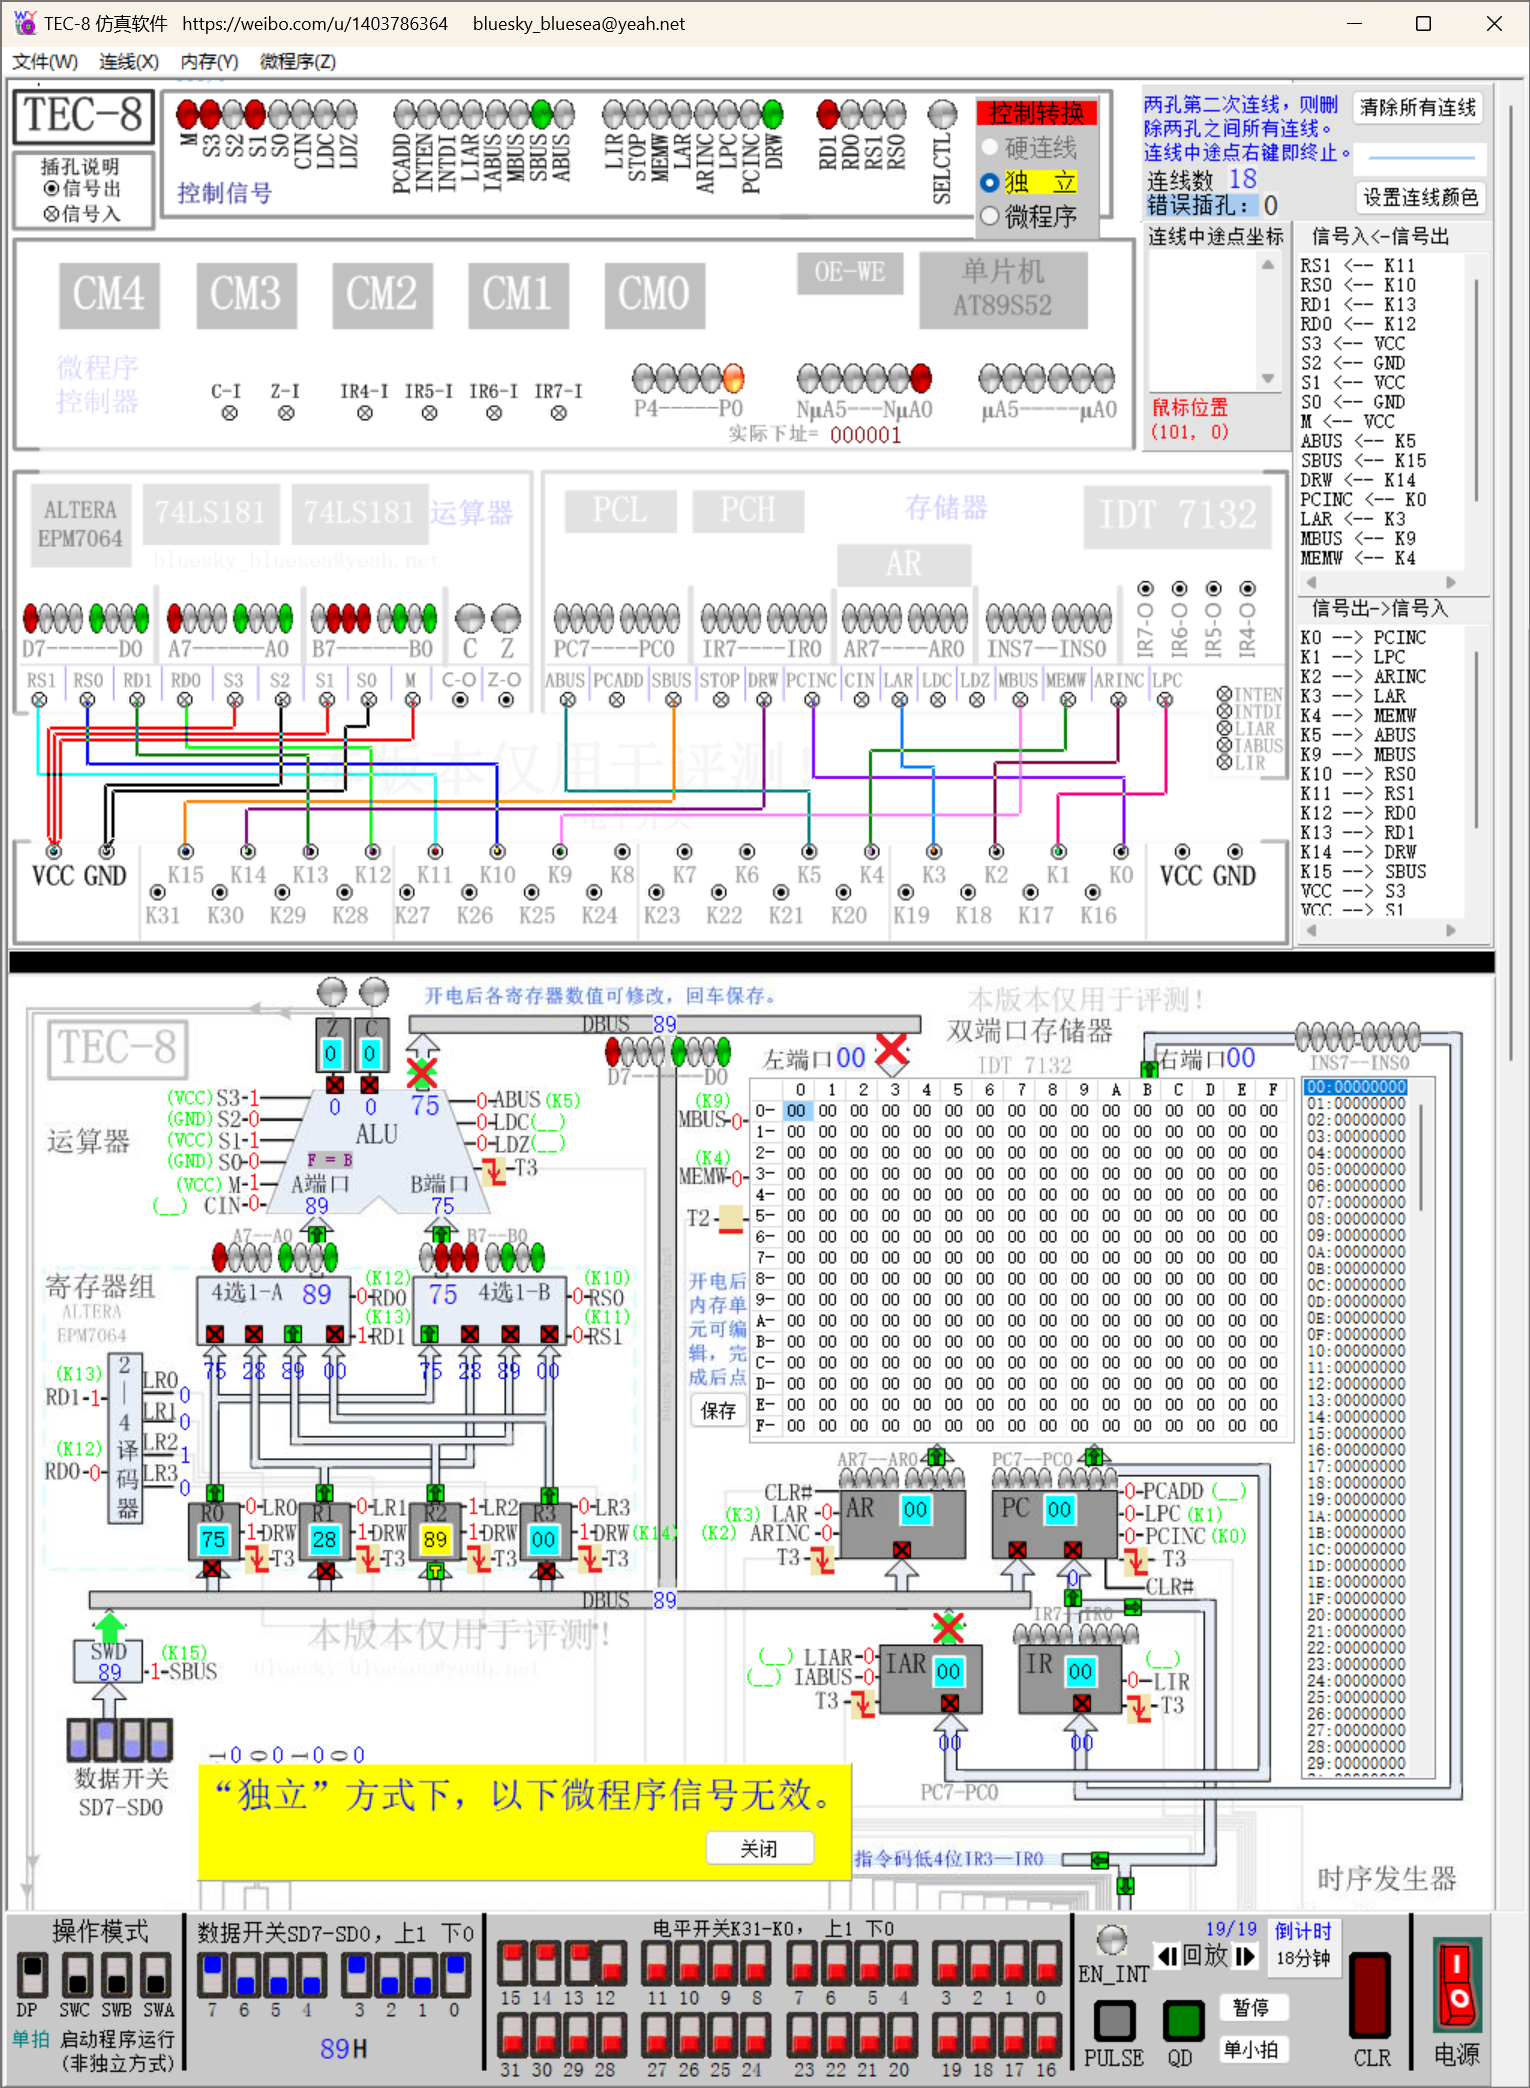
\includegraphics[width=0.3\textwidth]{screenshots/3.2.4.png}
              }
              \subfigure[将数 32H 写到 R$_3$]{
                  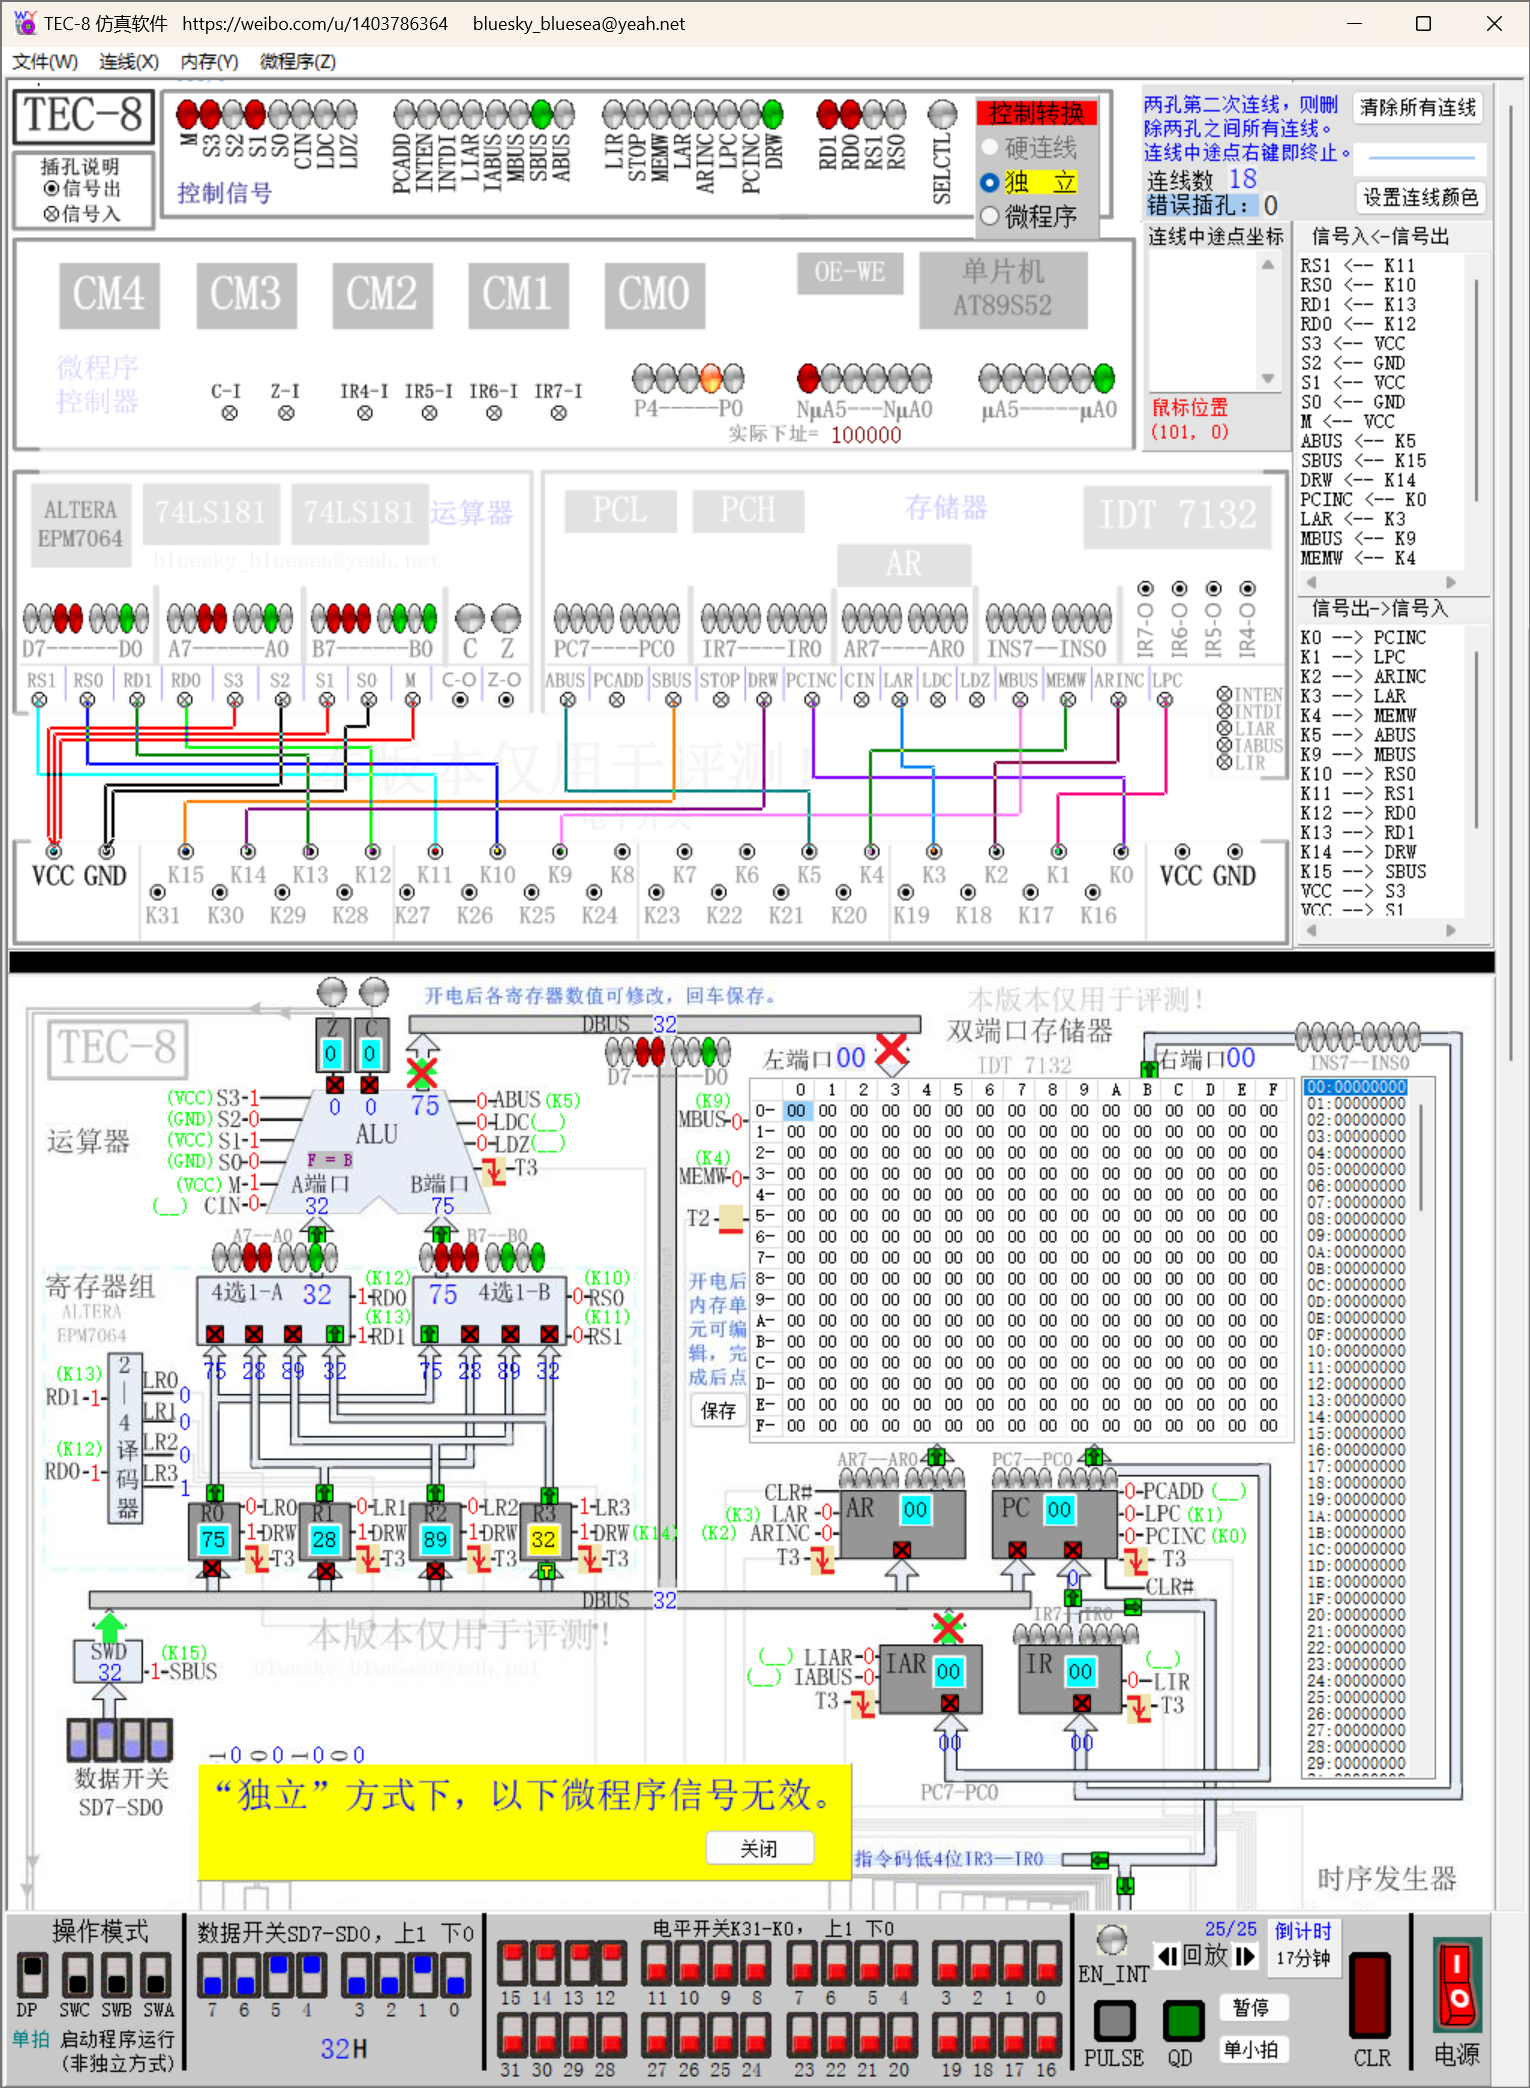
\includegraphics[width=0.3\textwidth]{screenshots/3.2.5.png}
              }
              \caption{写入数据 (独立)}
              \label{fig:3.7}
          \end{figure}

    \item 设置存储器地址 AR 和程序计数器 PC 为 20H. (如图 \ref{fig:3.8} 所示.)

          \begin{figure}[htbp]
              \centering
              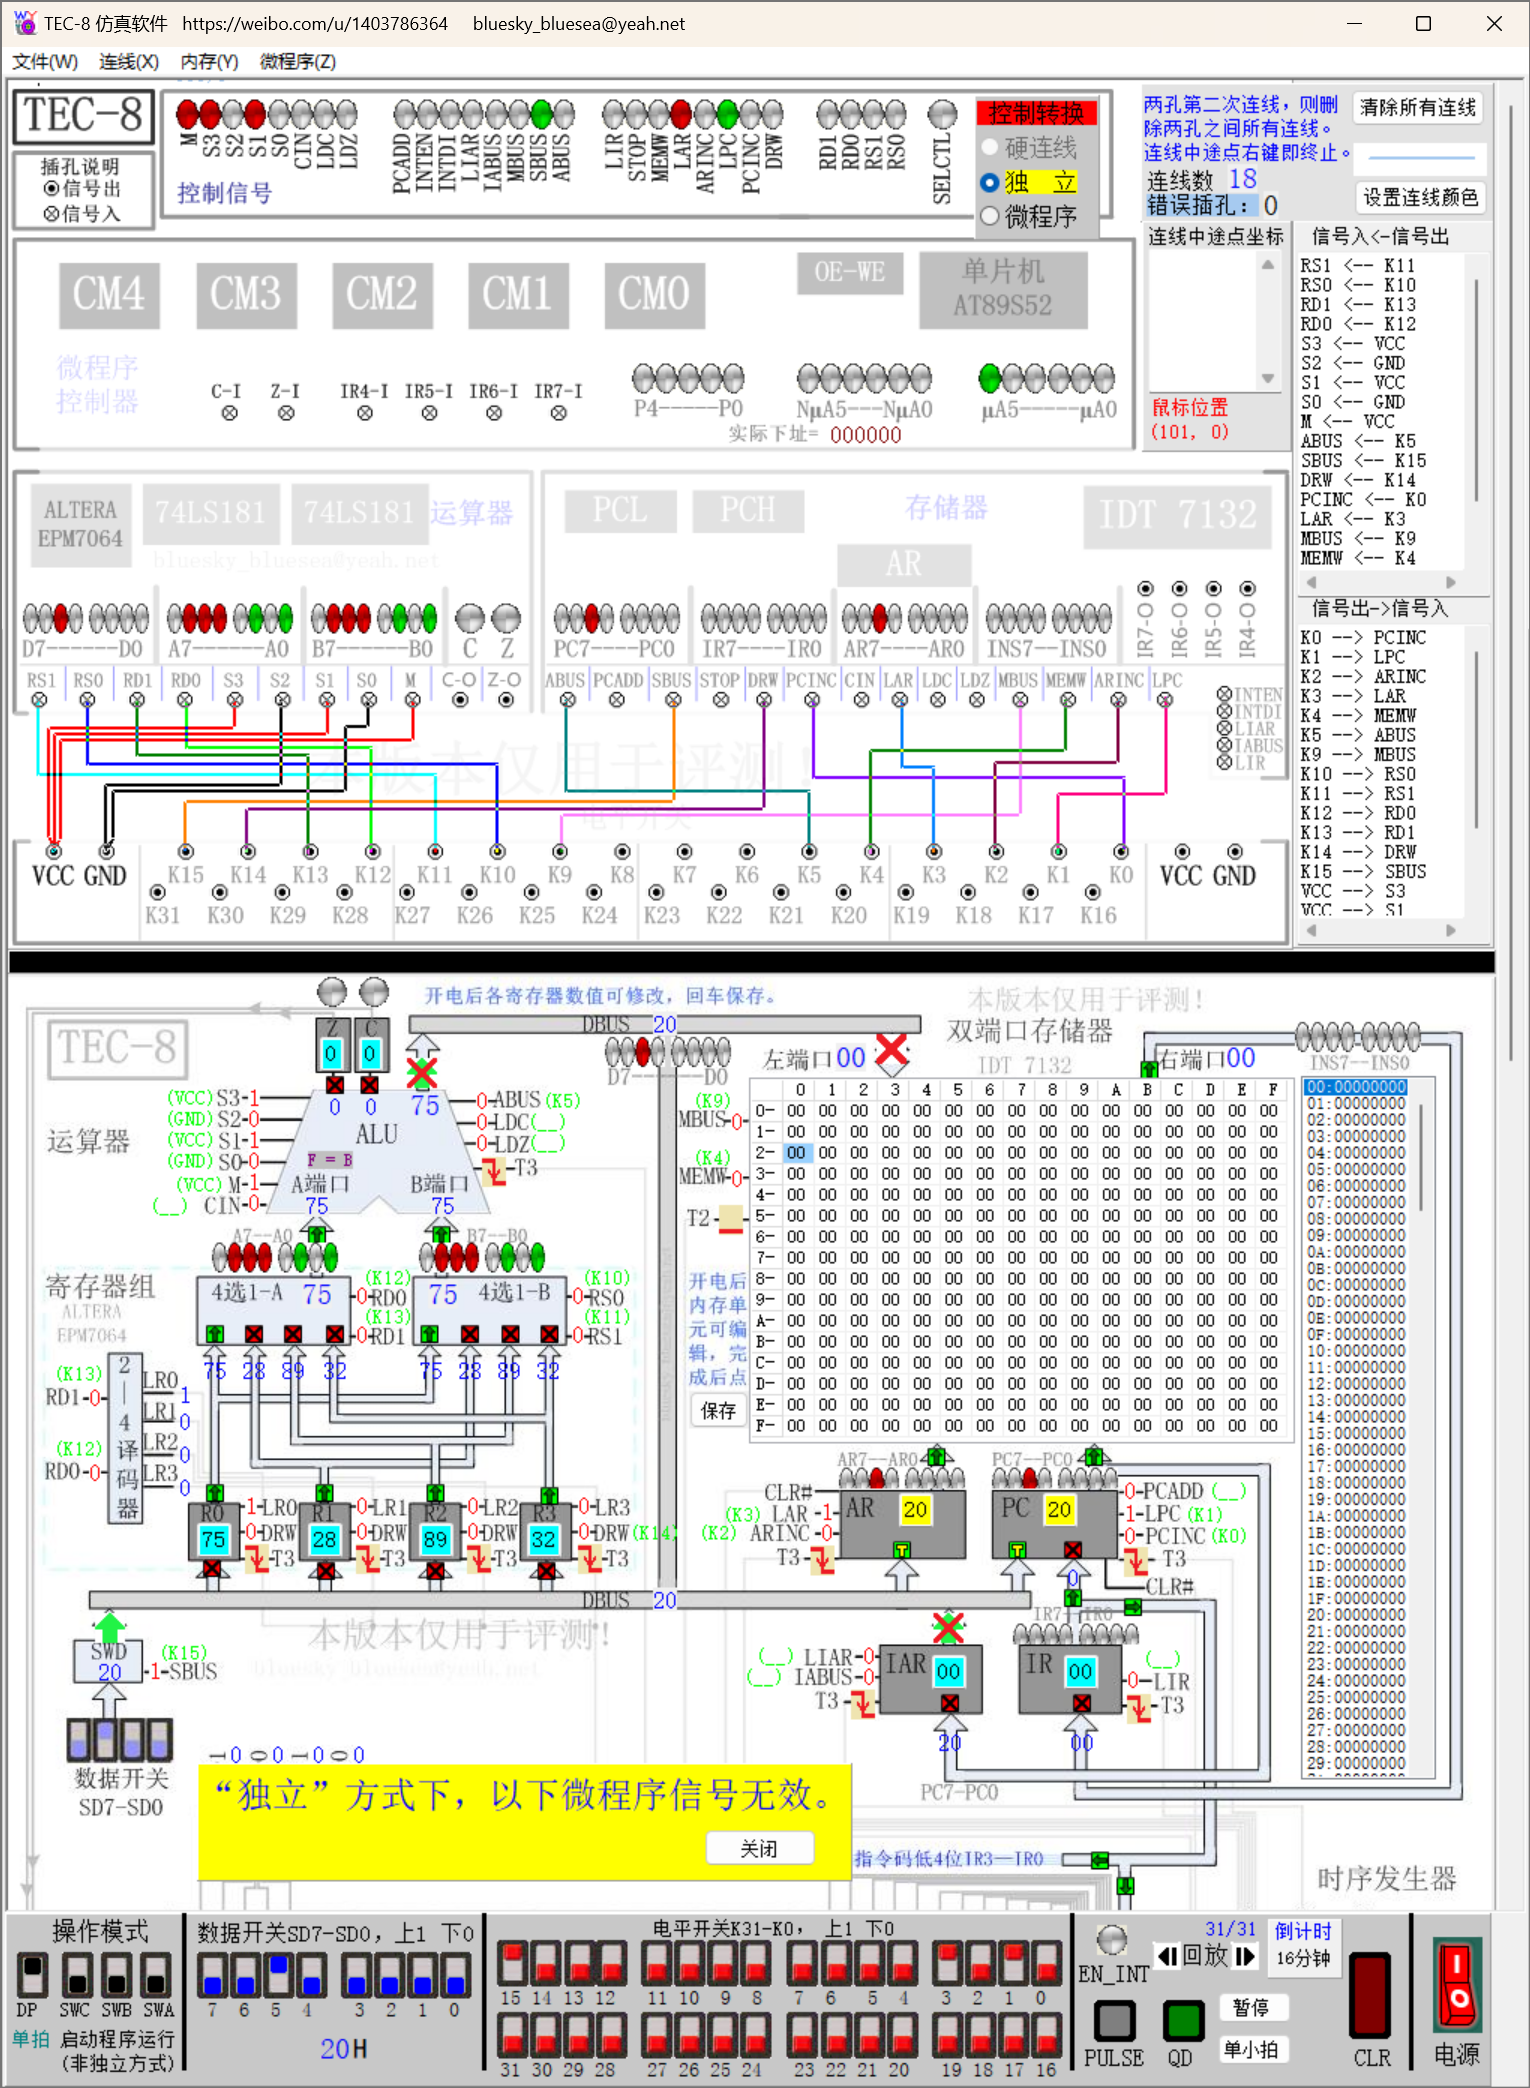
\includegraphics[width=0.3\textwidth]{screenshots/3.2.6.png}
              \caption{设置地址 (独立)}
              \label{fig:3.8}
          \end{figure}

    \item 将寄存器 R$_0$、R$_1$、R$_2$、R$_3$ 中的数依次写入存储器 20H、21H、22H 和 23H 单元. (如图 \ref{fig:3.9} 所示.)

          \begin{figure}[htbp]
              \centering
              \subfigure[将R$_0$数值写入20H单元]{
                  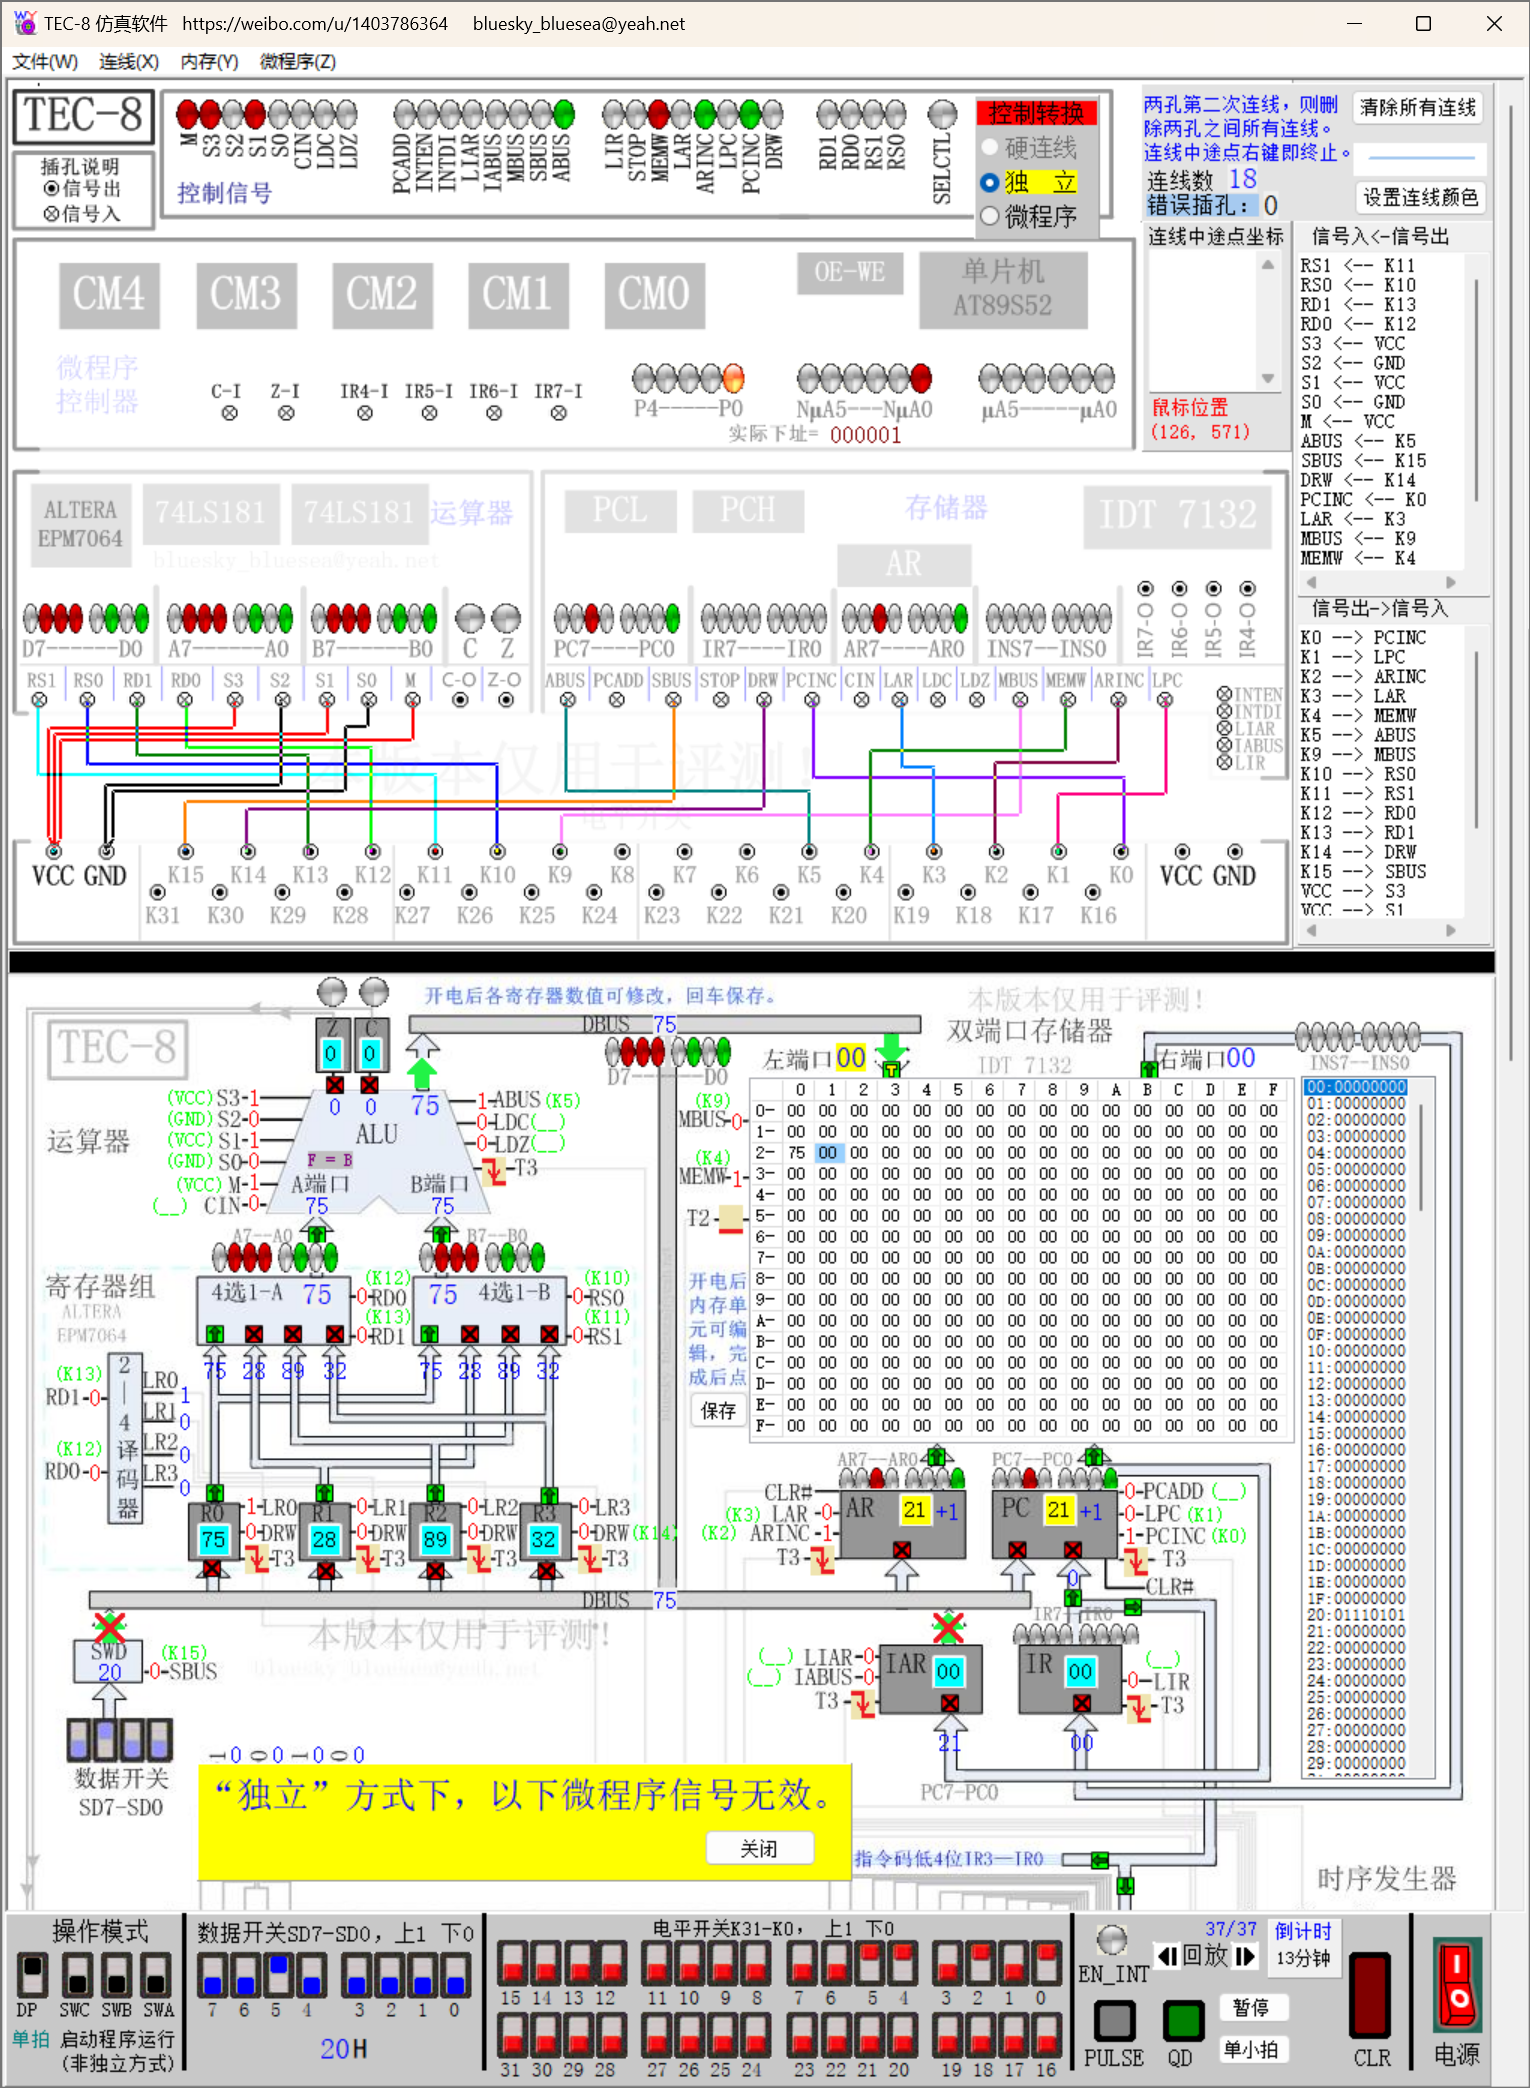
\includegraphics[width=0.3\textwidth]{screenshots/3.2.7.png}
              }
              \subfigure[将R$_1$数值写入21H单元]{
                  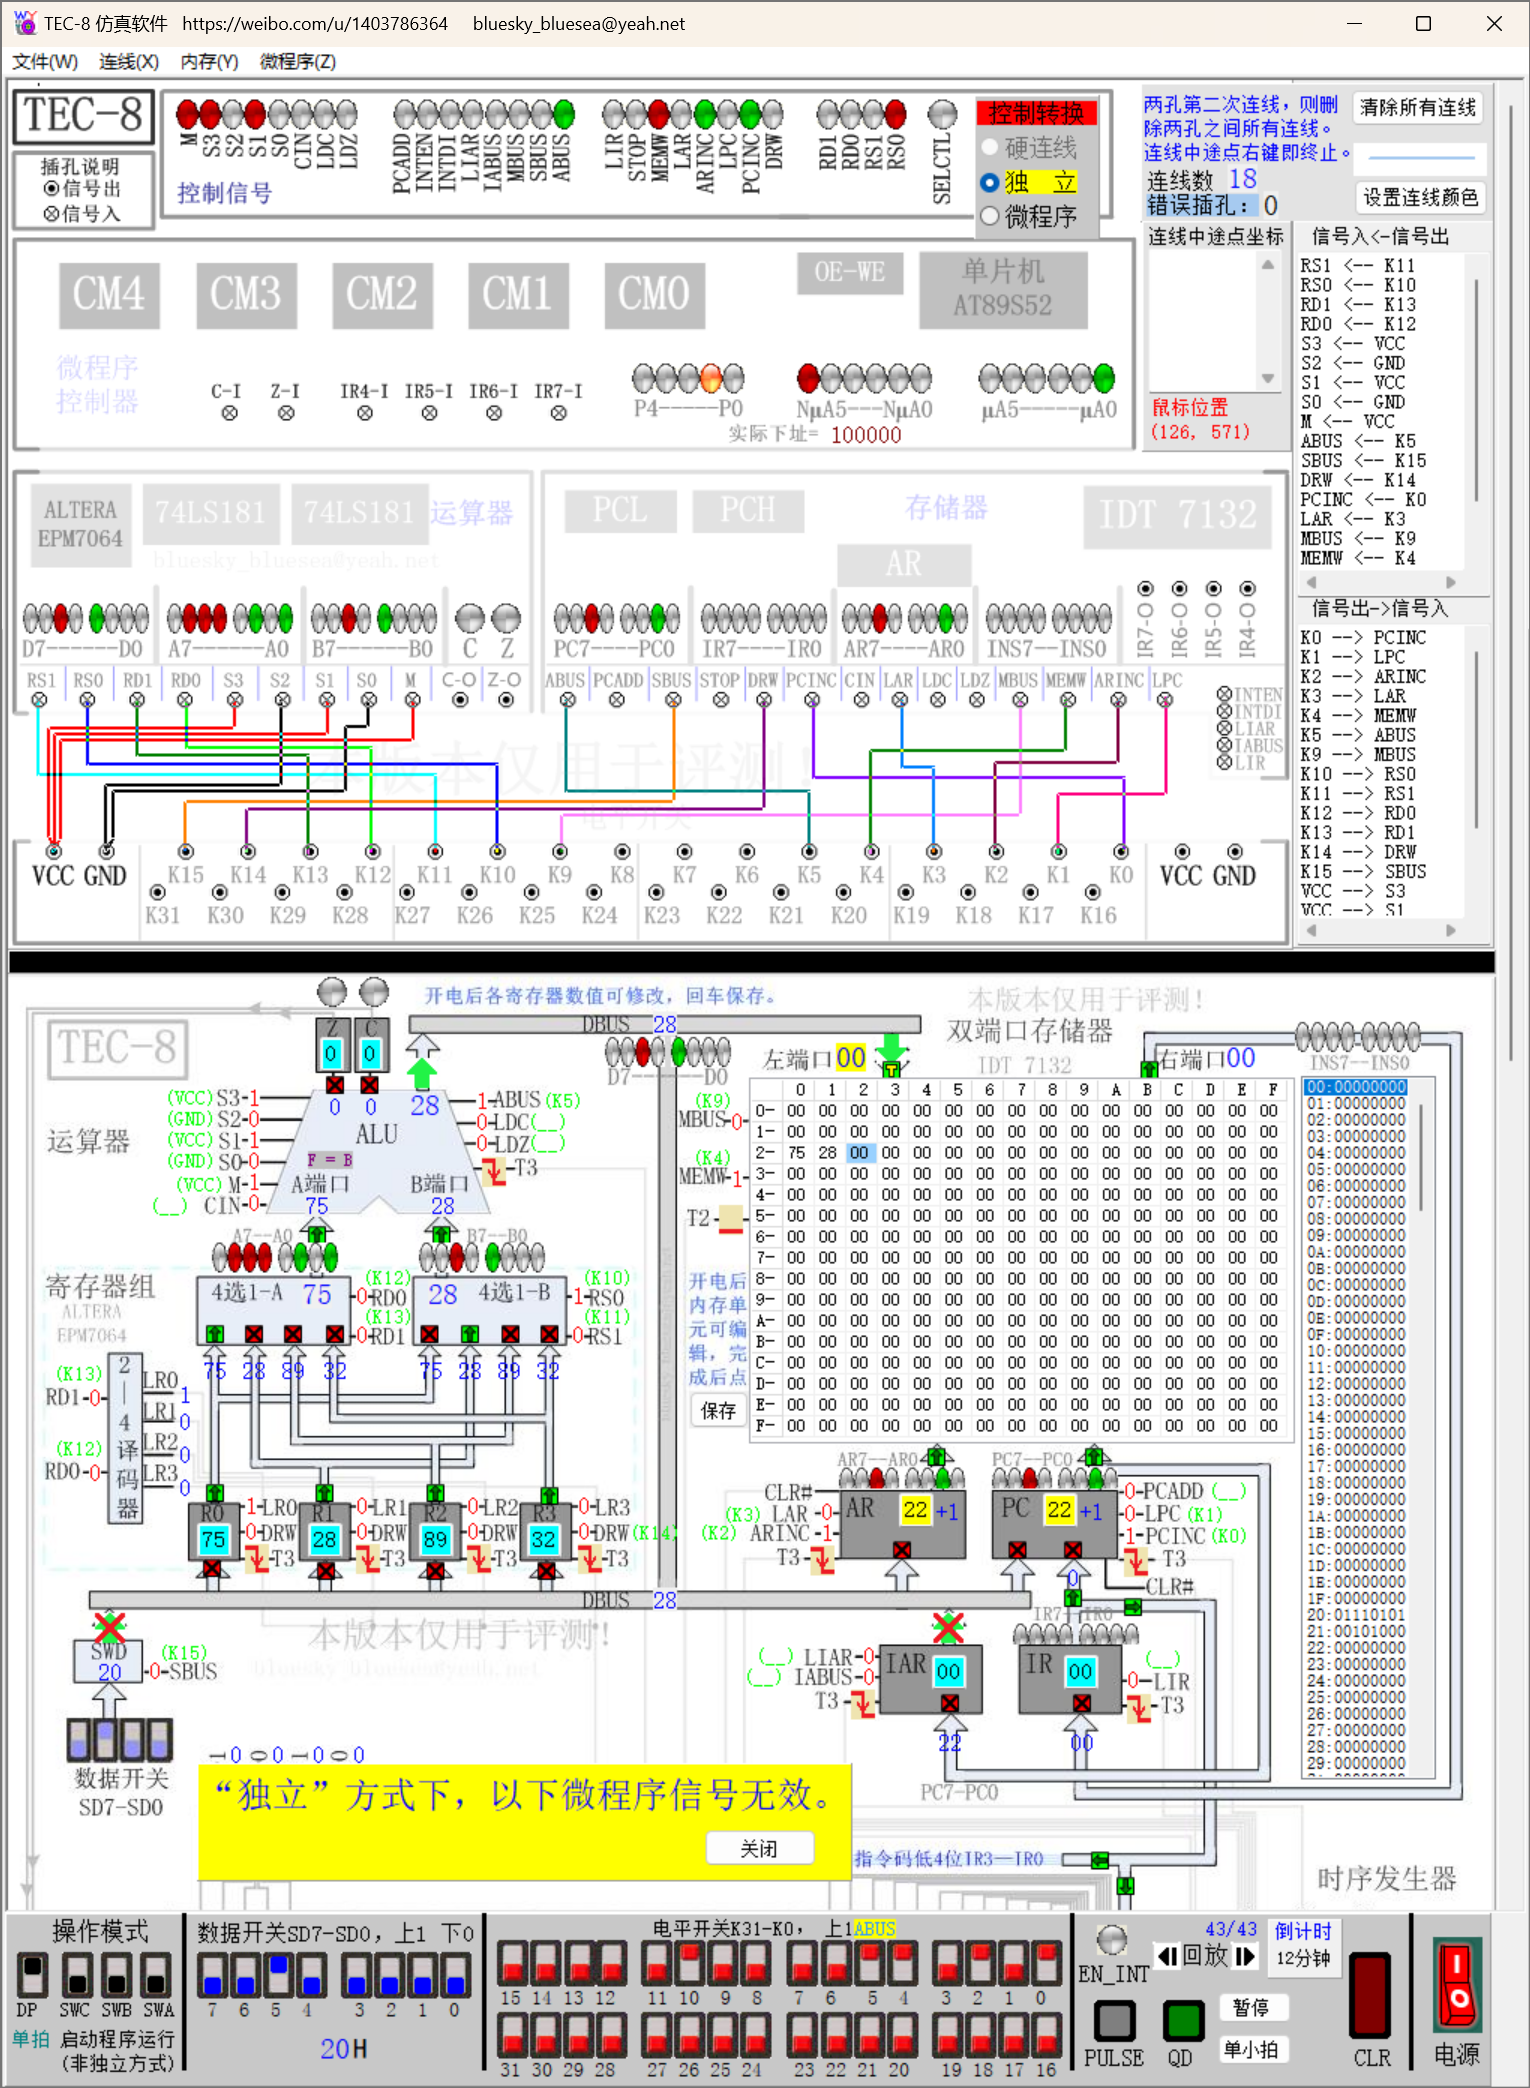
\includegraphics[width=0.3\textwidth]{screenshots/3.2.8.png}
              }
              \\
              \subfigure[将R$_2$数值写入22H单元]{
                  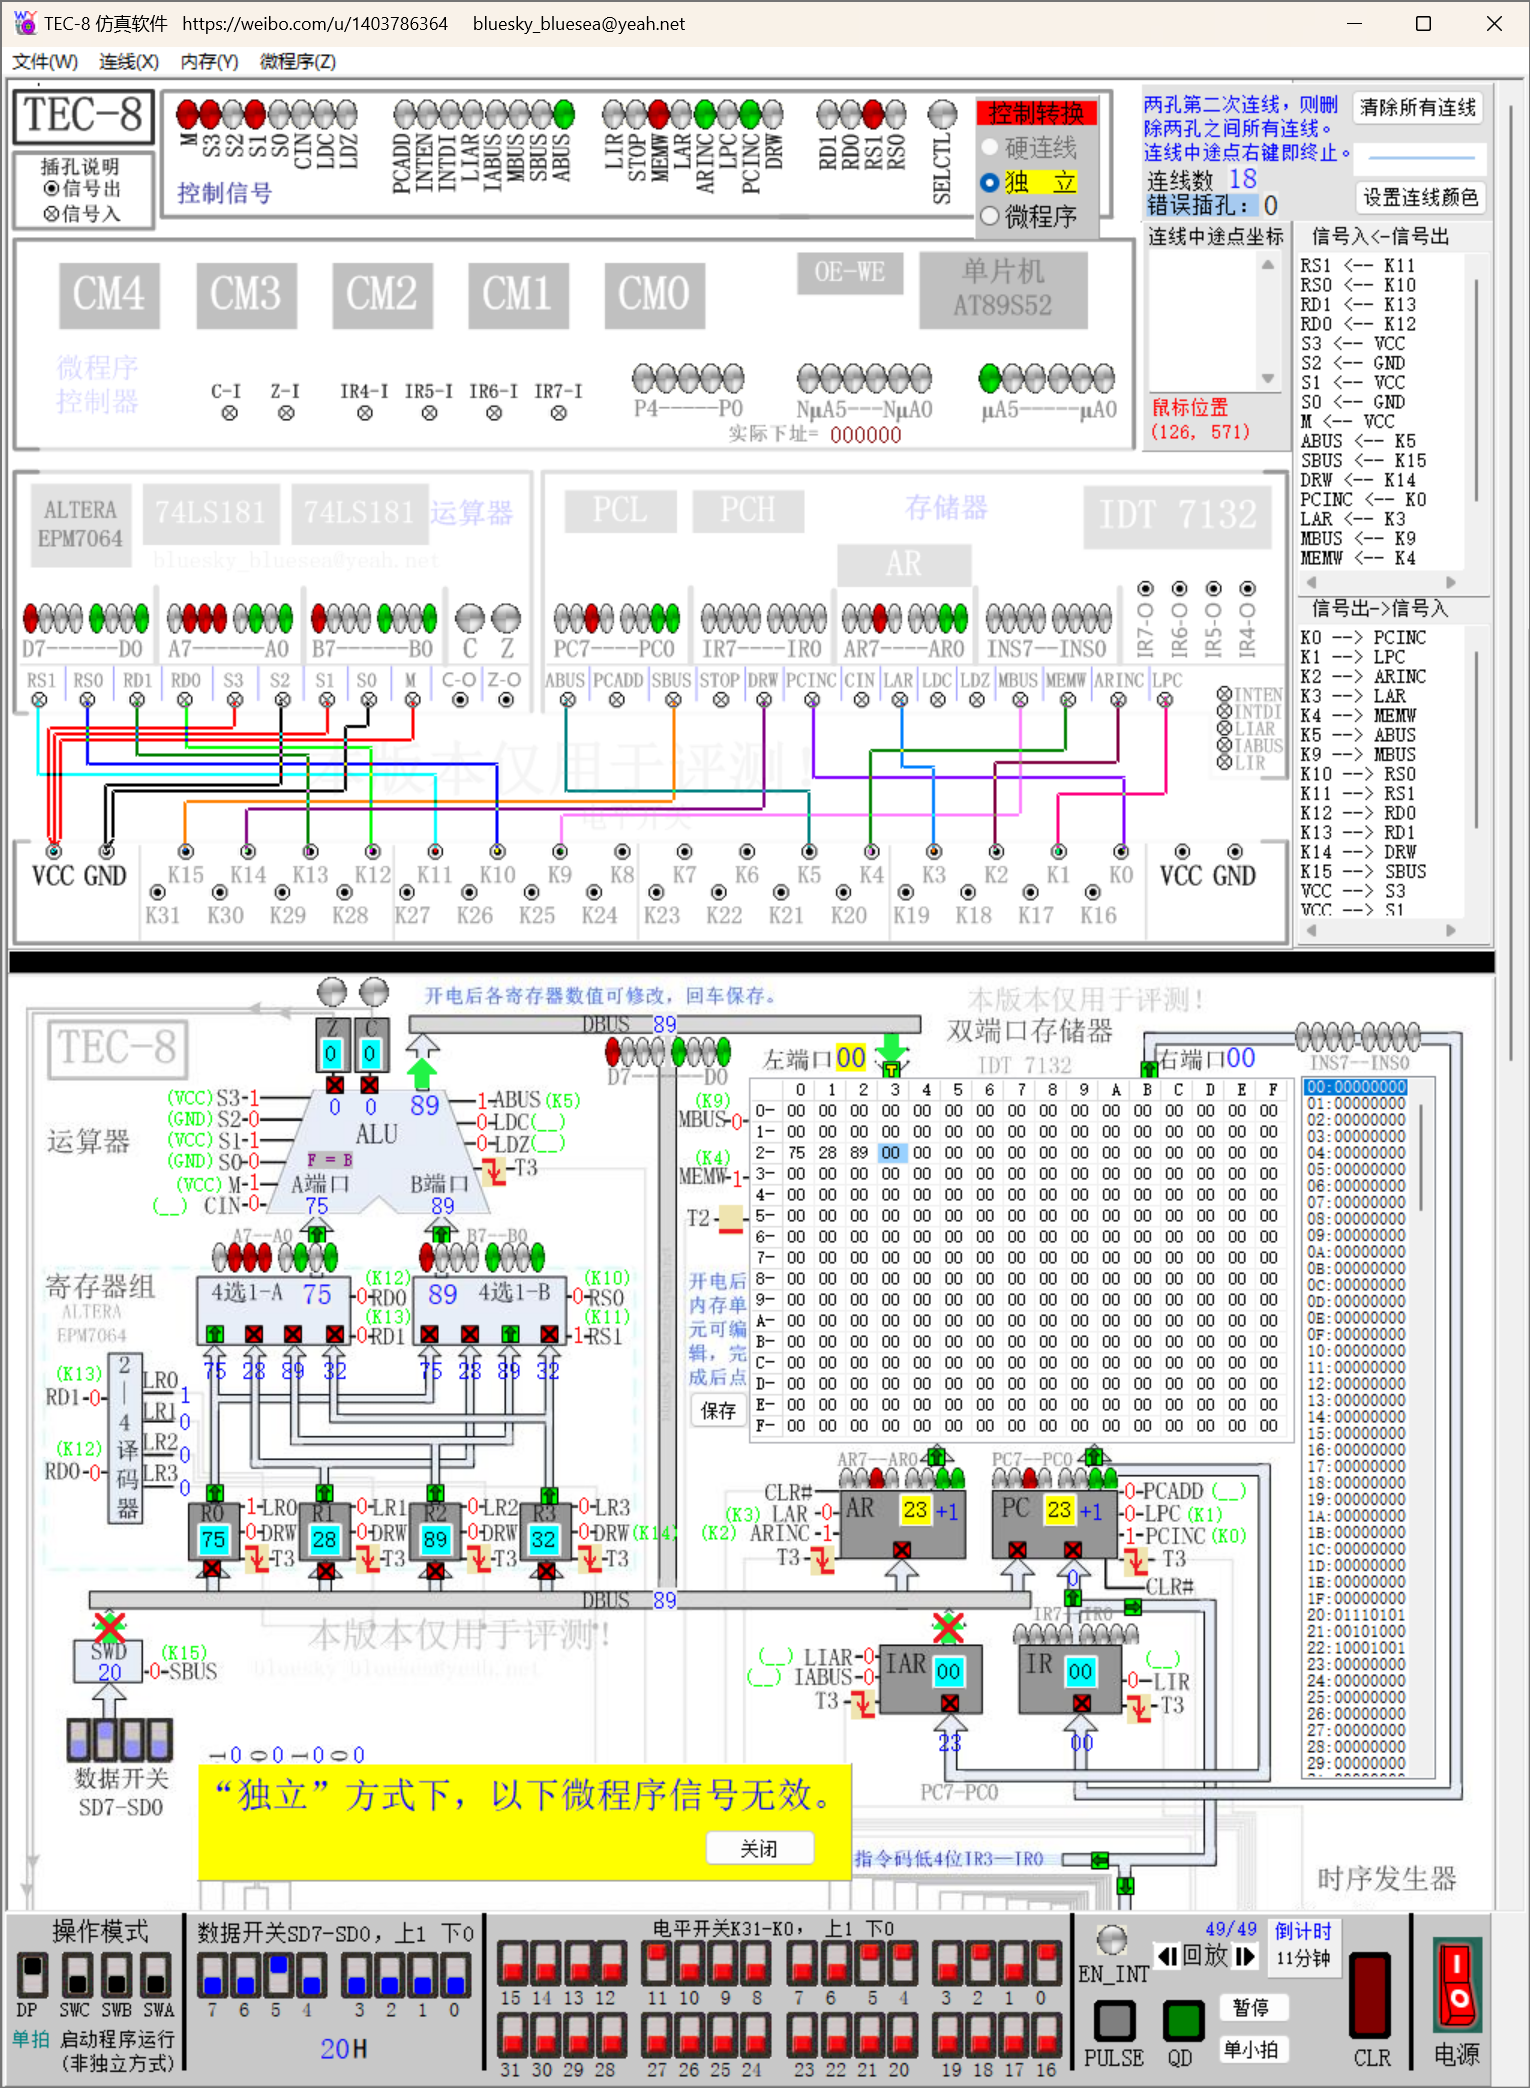
\includegraphics[width=0.3\textwidth]{screenshots/3.2.9.png}
              }
              \subfigure[将R$_3$数值写入23H单元]{
                  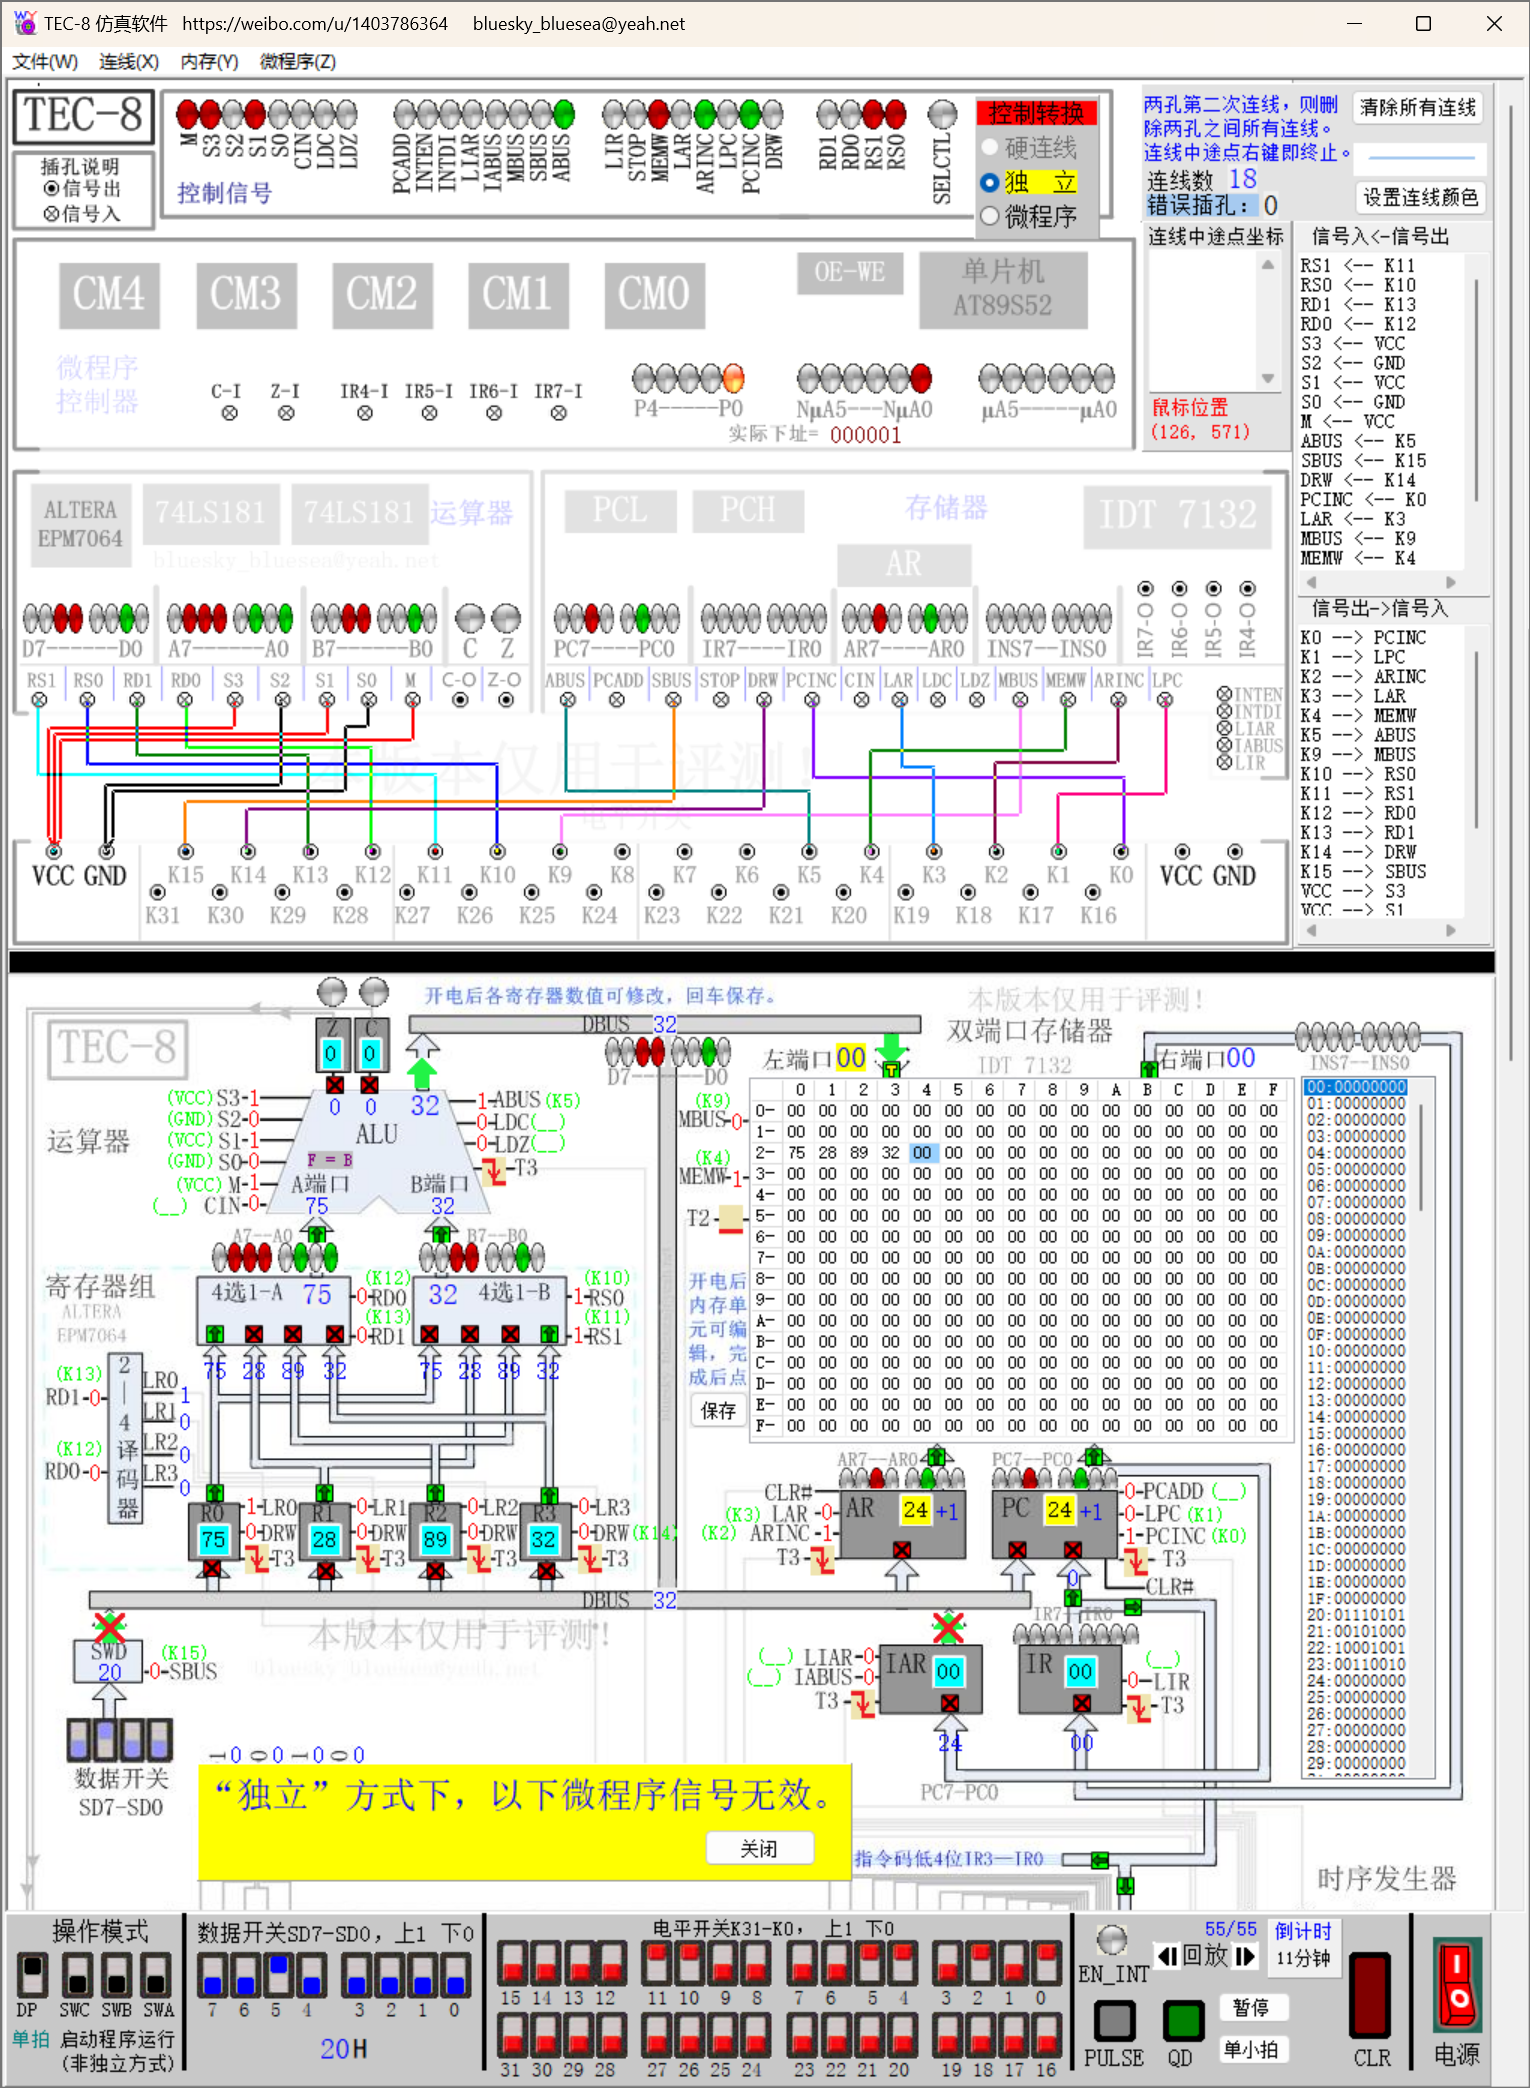
\includegraphics[width=0.3\textwidth]{screenshots/3.2.10.png}
              }
              \caption{写入存储器 (独立)}
              \label{fig:3.9}
          \end{figure}

    \item 重新设置存储器地址 AR 和程序计数器 PC 为 20H. (如图 \ref{fig:3.10} 所示.)

          \begin{figure}[htbp]
              \centering
              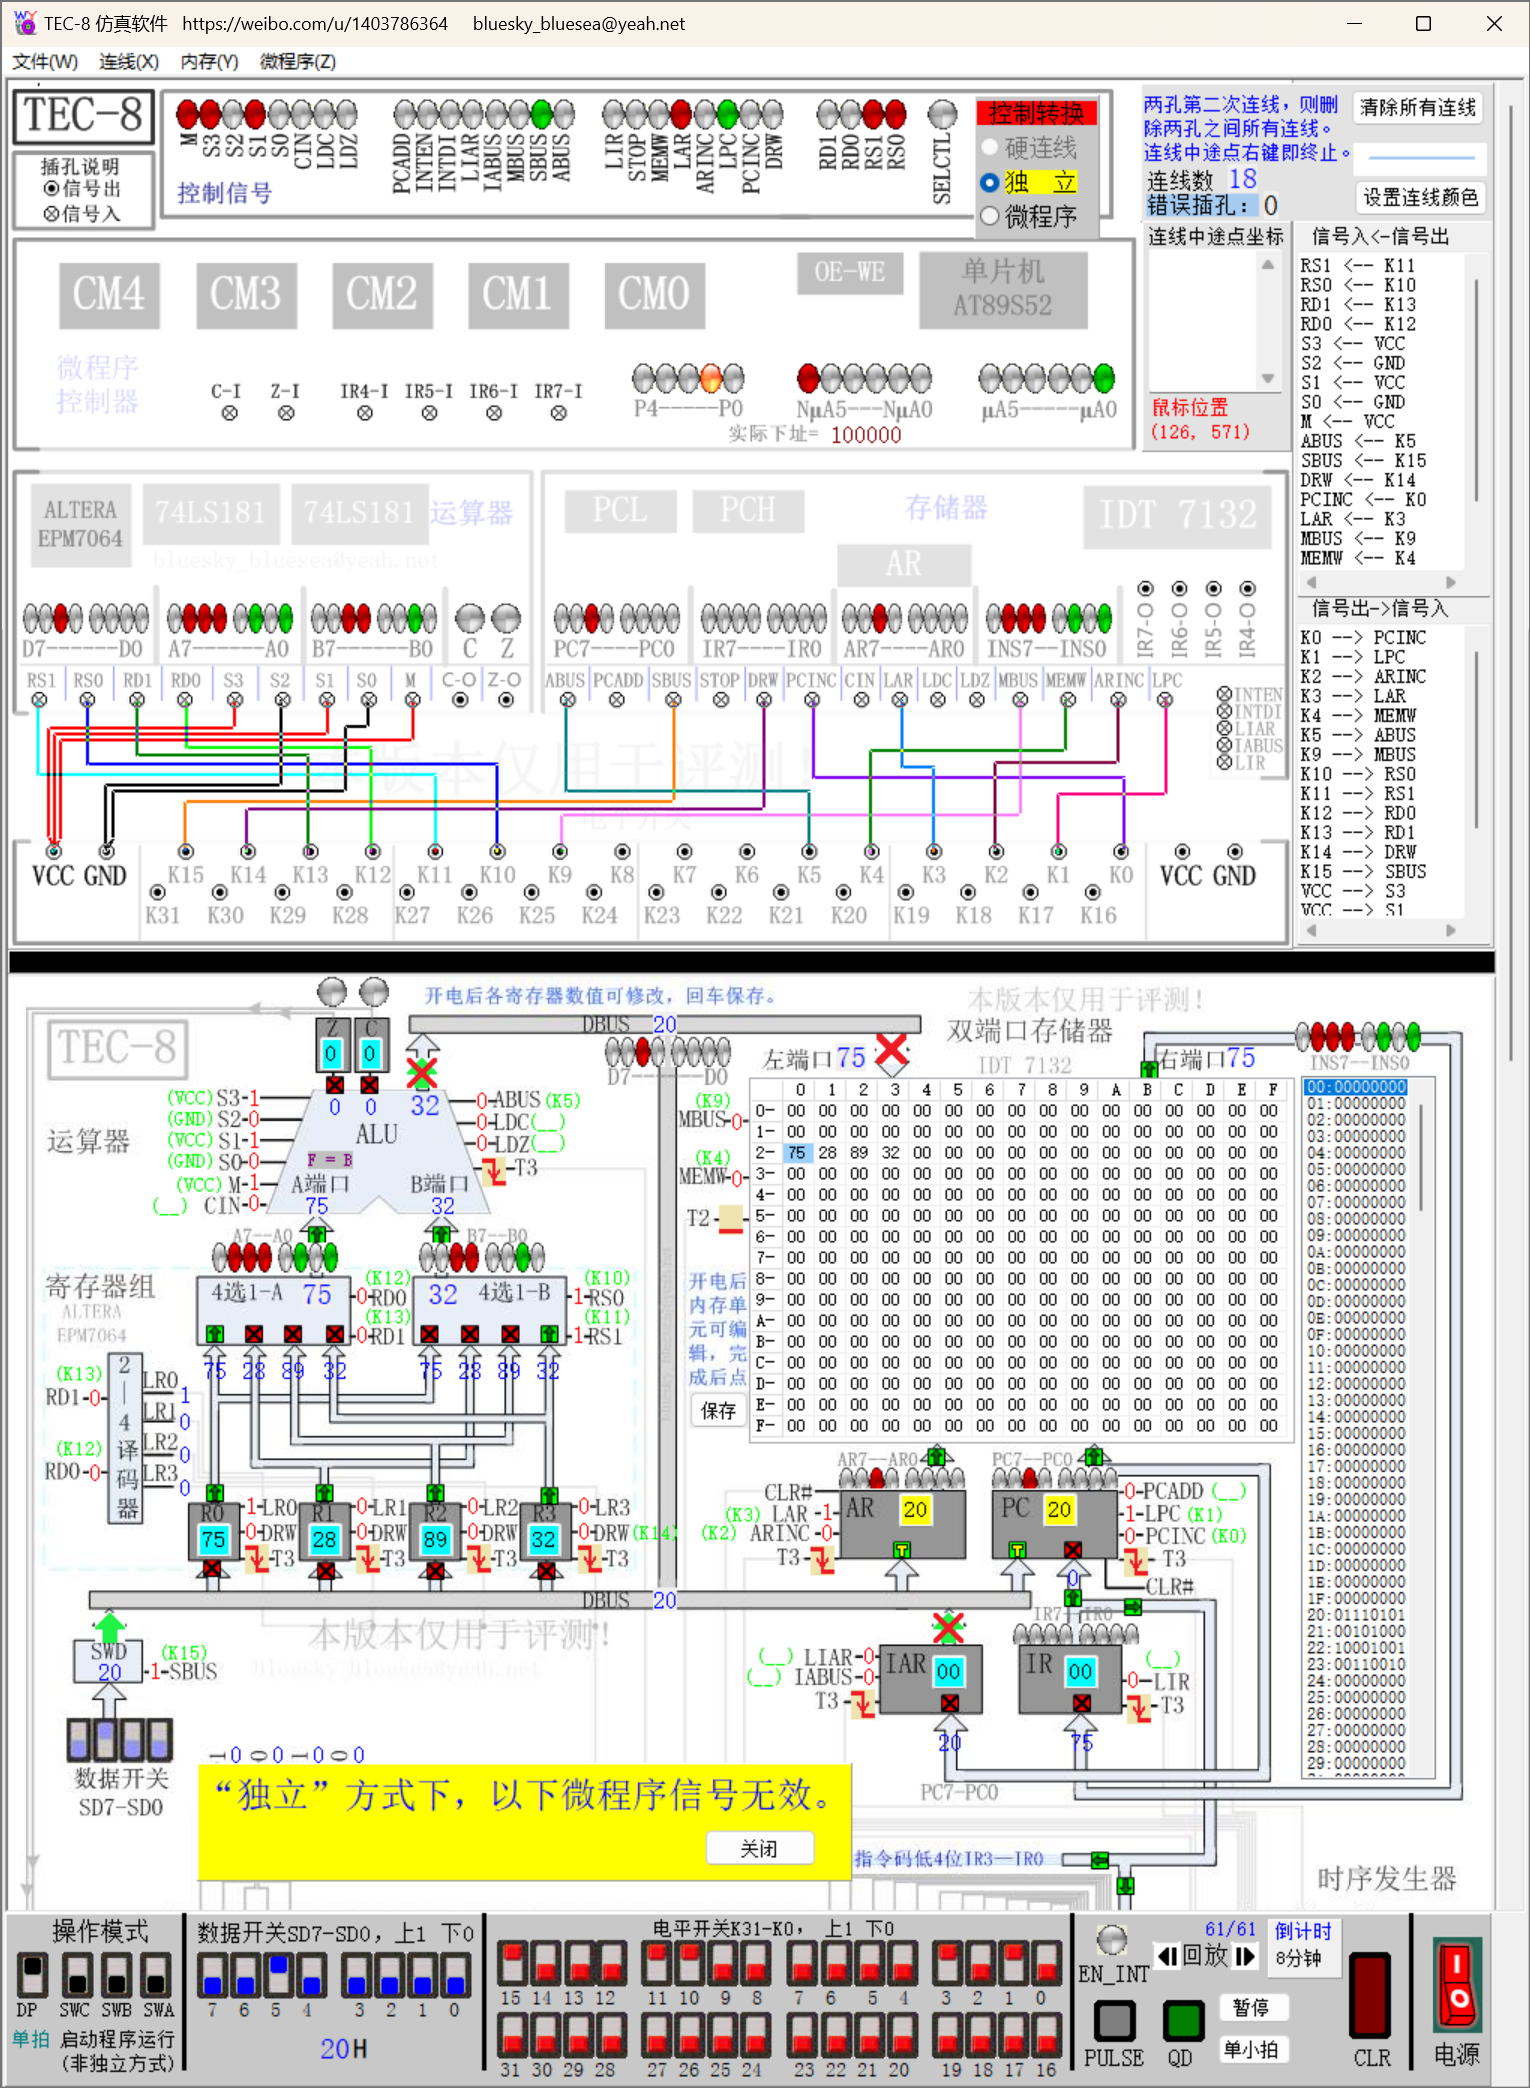
\includegraphics[width=0.3\textwidth]{screenshots/3.2.11.png}
              \caption{重设地址 (独立)}
              \label{fig:3.10}
          \end{figure}

    \item 将存储器 20H、21H、22H 和 23H 单元中的数依次写入寄存器 R$_3$、R$_2$、R$_1$ 和 R$_0$. (如图 \ref{fig:3.11} 所示.)

          \begin{figure}[htbp]
              \centering
              \subfigure[将20H单元的数值写入R$_3$]{
                  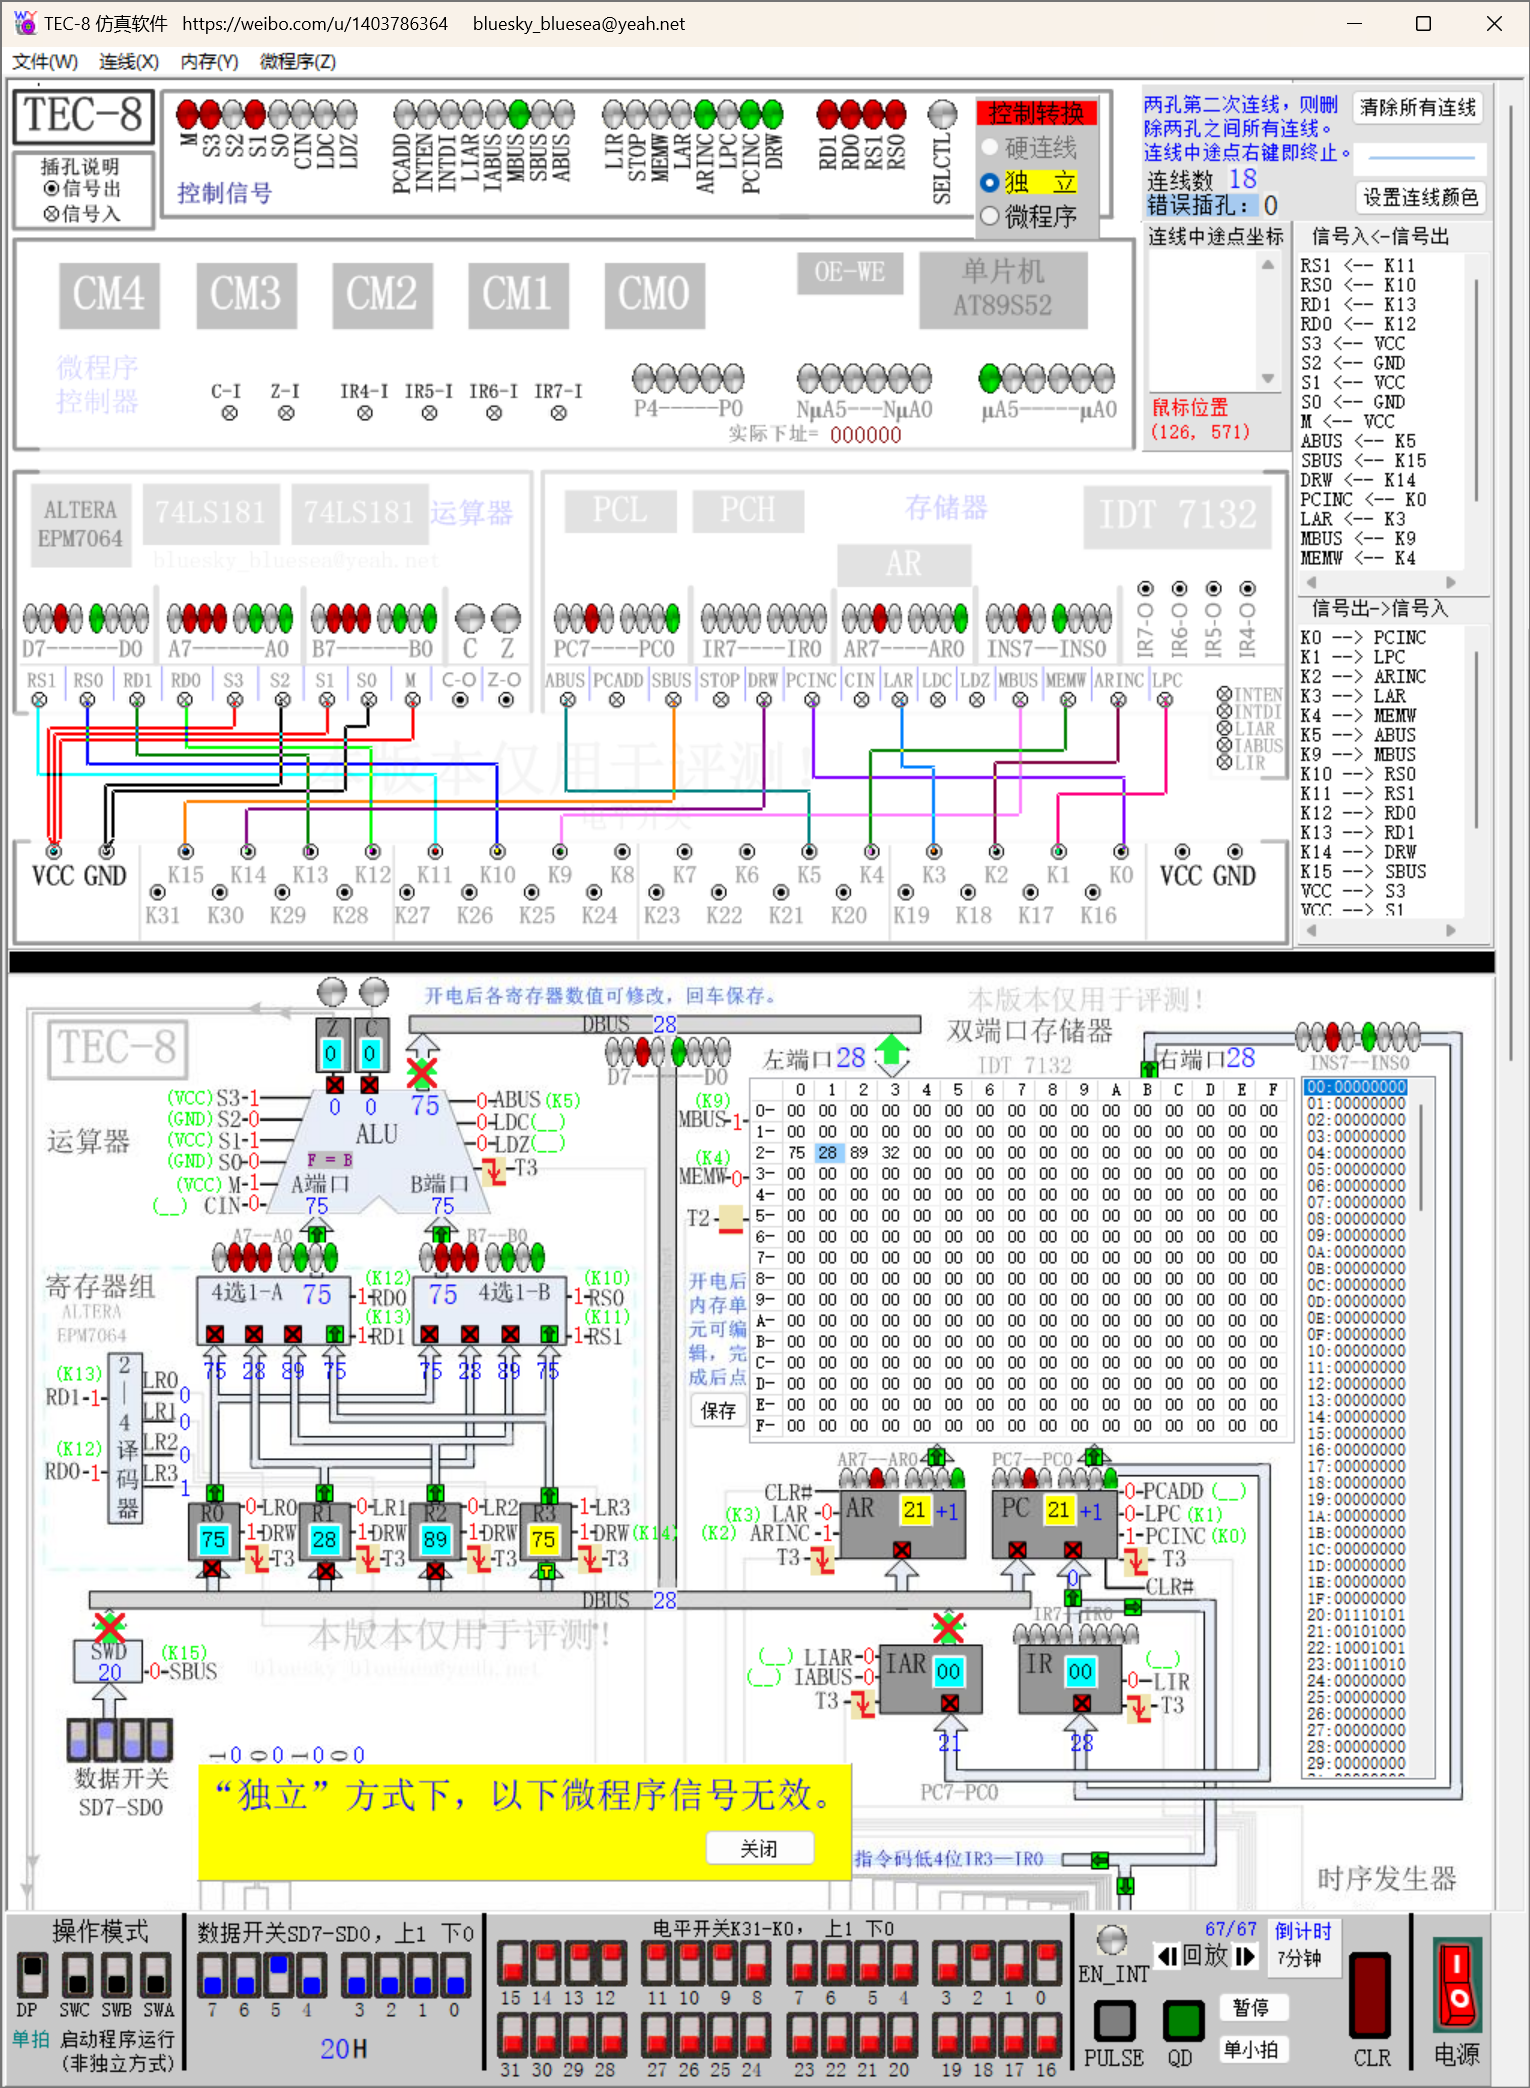
\includegraphics[width=0.3\textwidth]{screenshots/3.2.12.png}
              }
              \subfigure[将21H单元的数值写入R$_2$]{
                  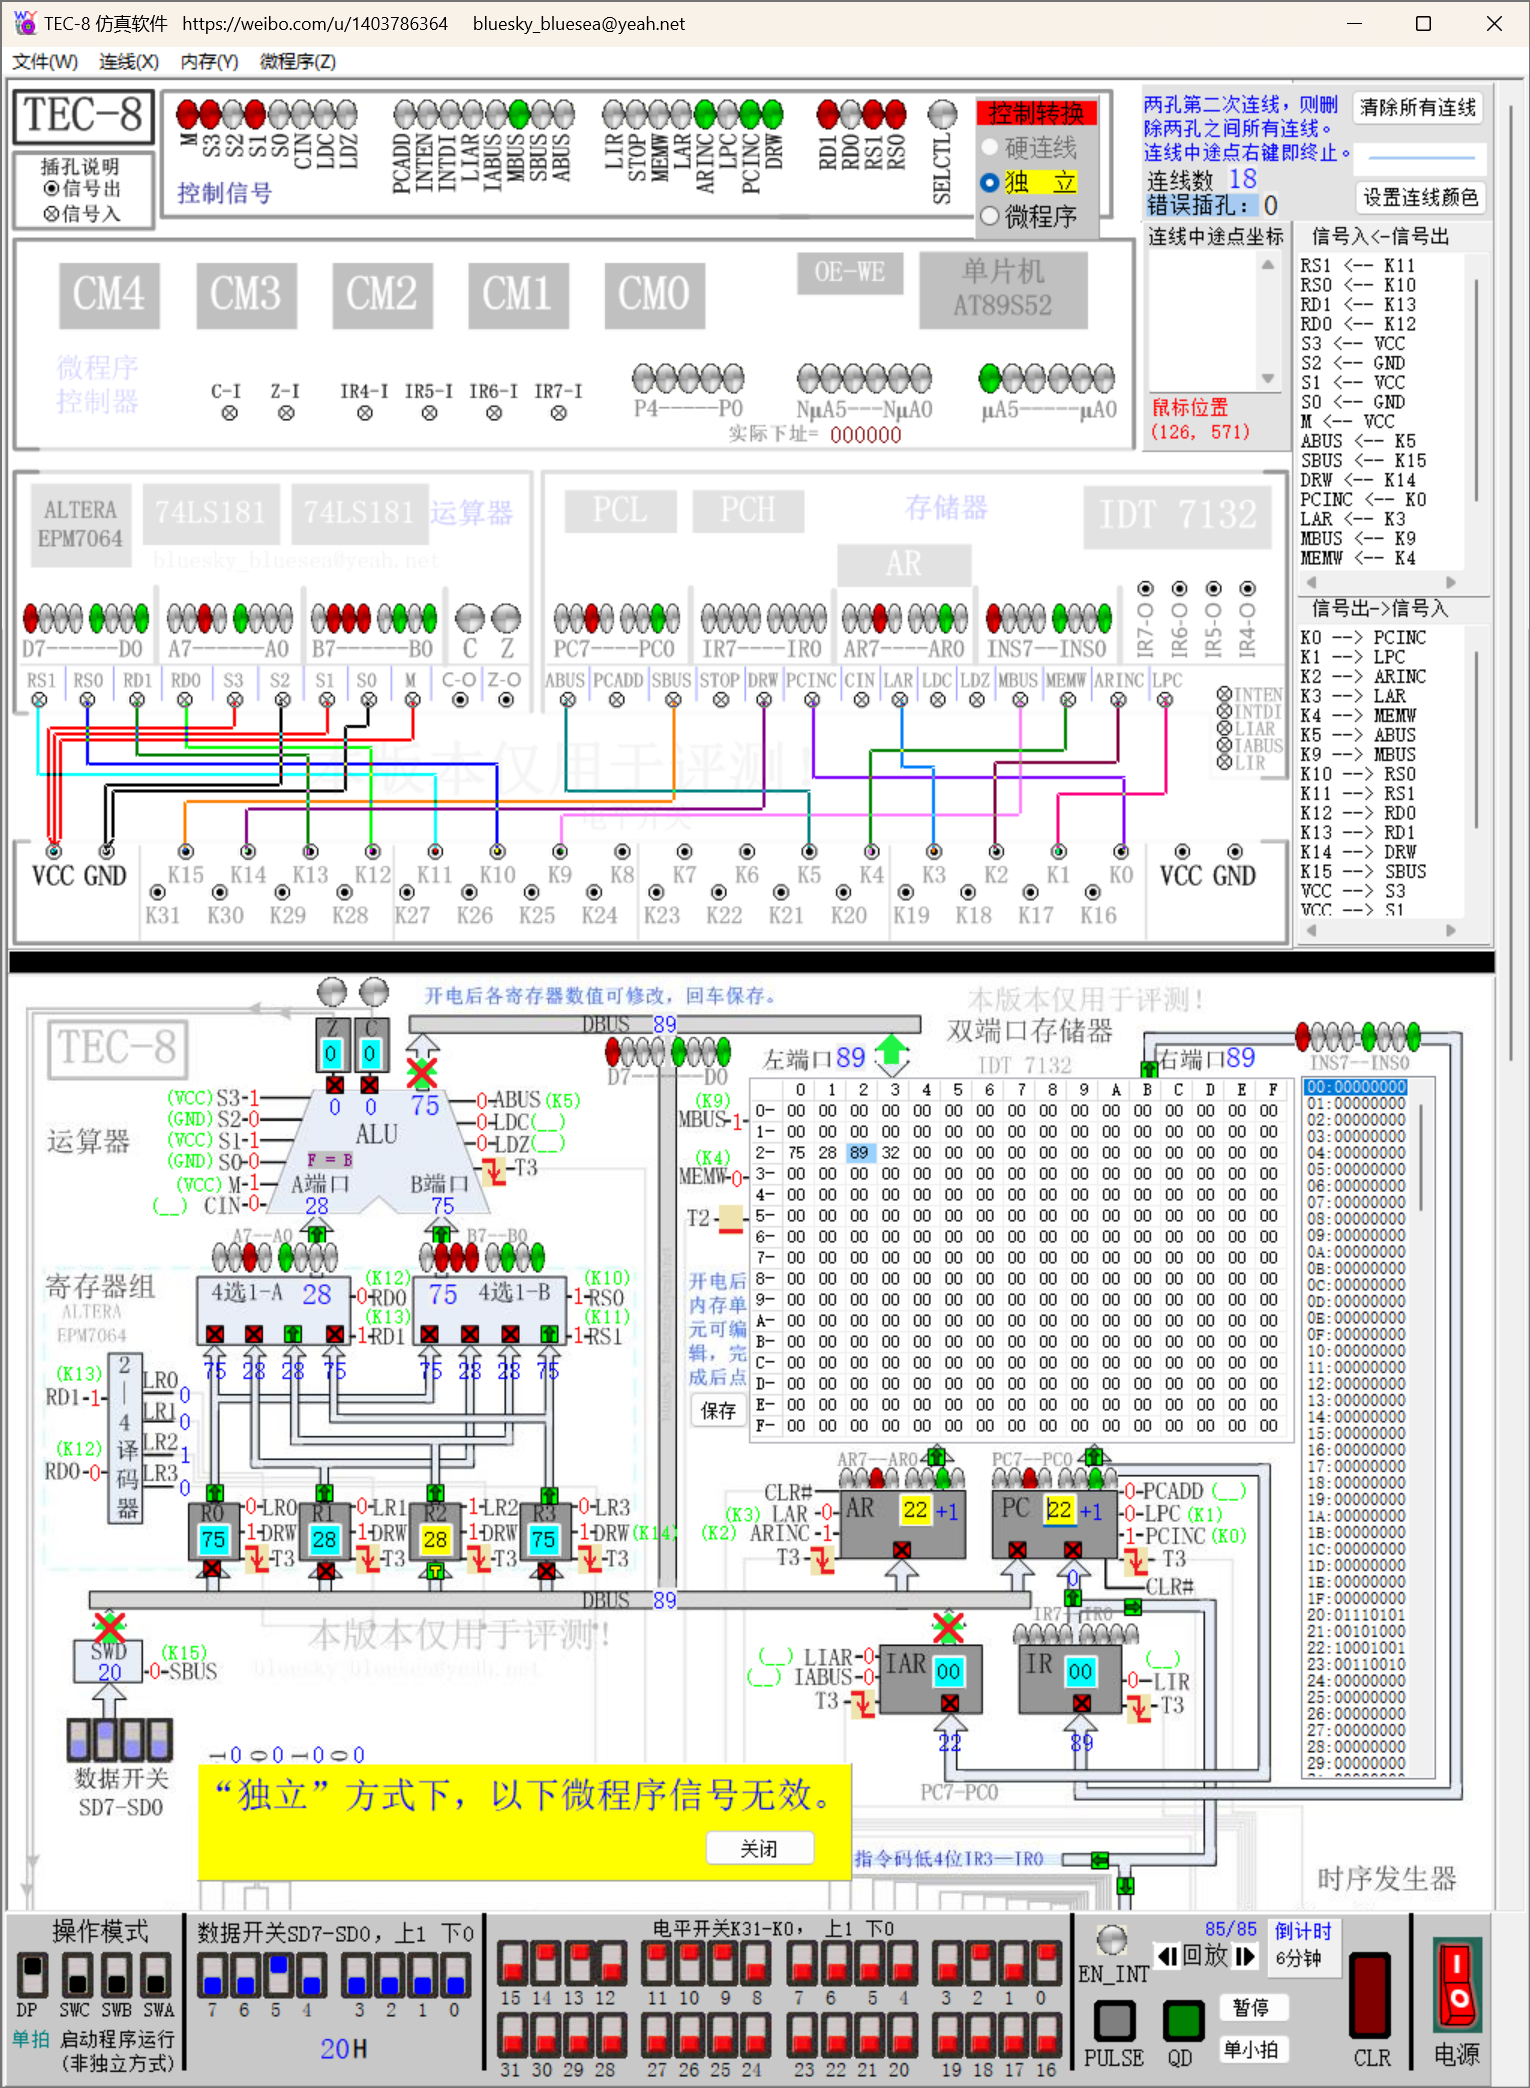
\includegraphics[width=0.3\textwidth]{screenshots/3.2.13.png}
              }
              \\
              \subfigure[将22H单元的数值写入R$_1$]{
                  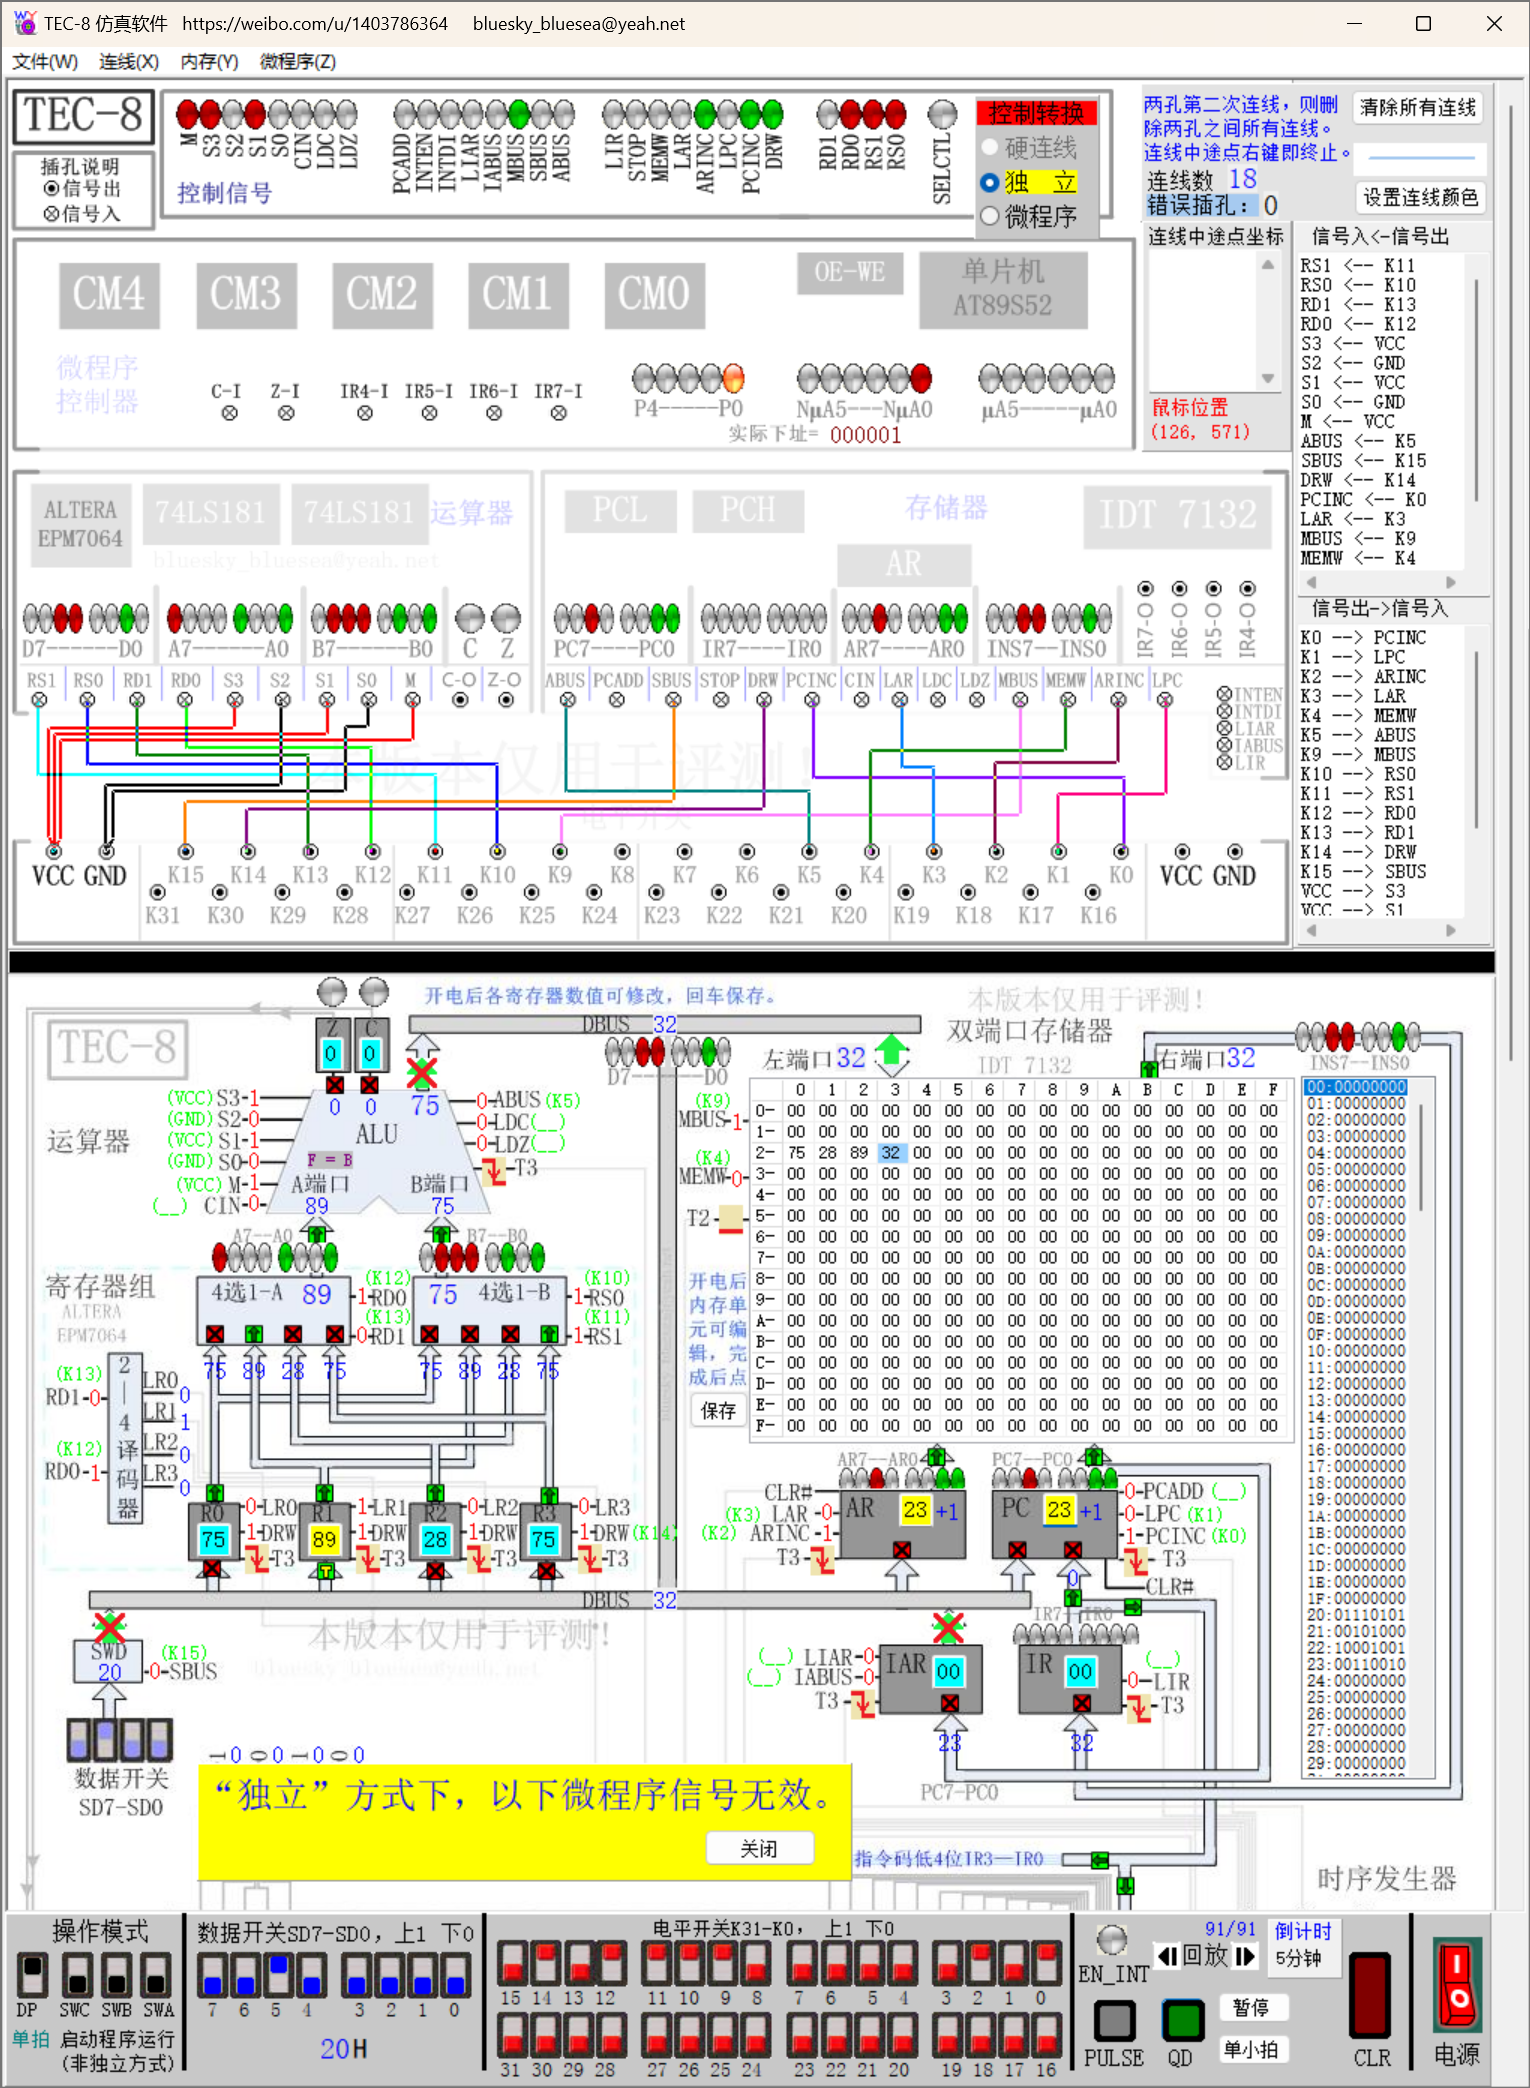
\includegraphics[width=0.3\textwidth]{screenshots/3.2.14.png}
              }
              \subfigure[将23H单元的数值写入R$_0$]{
                  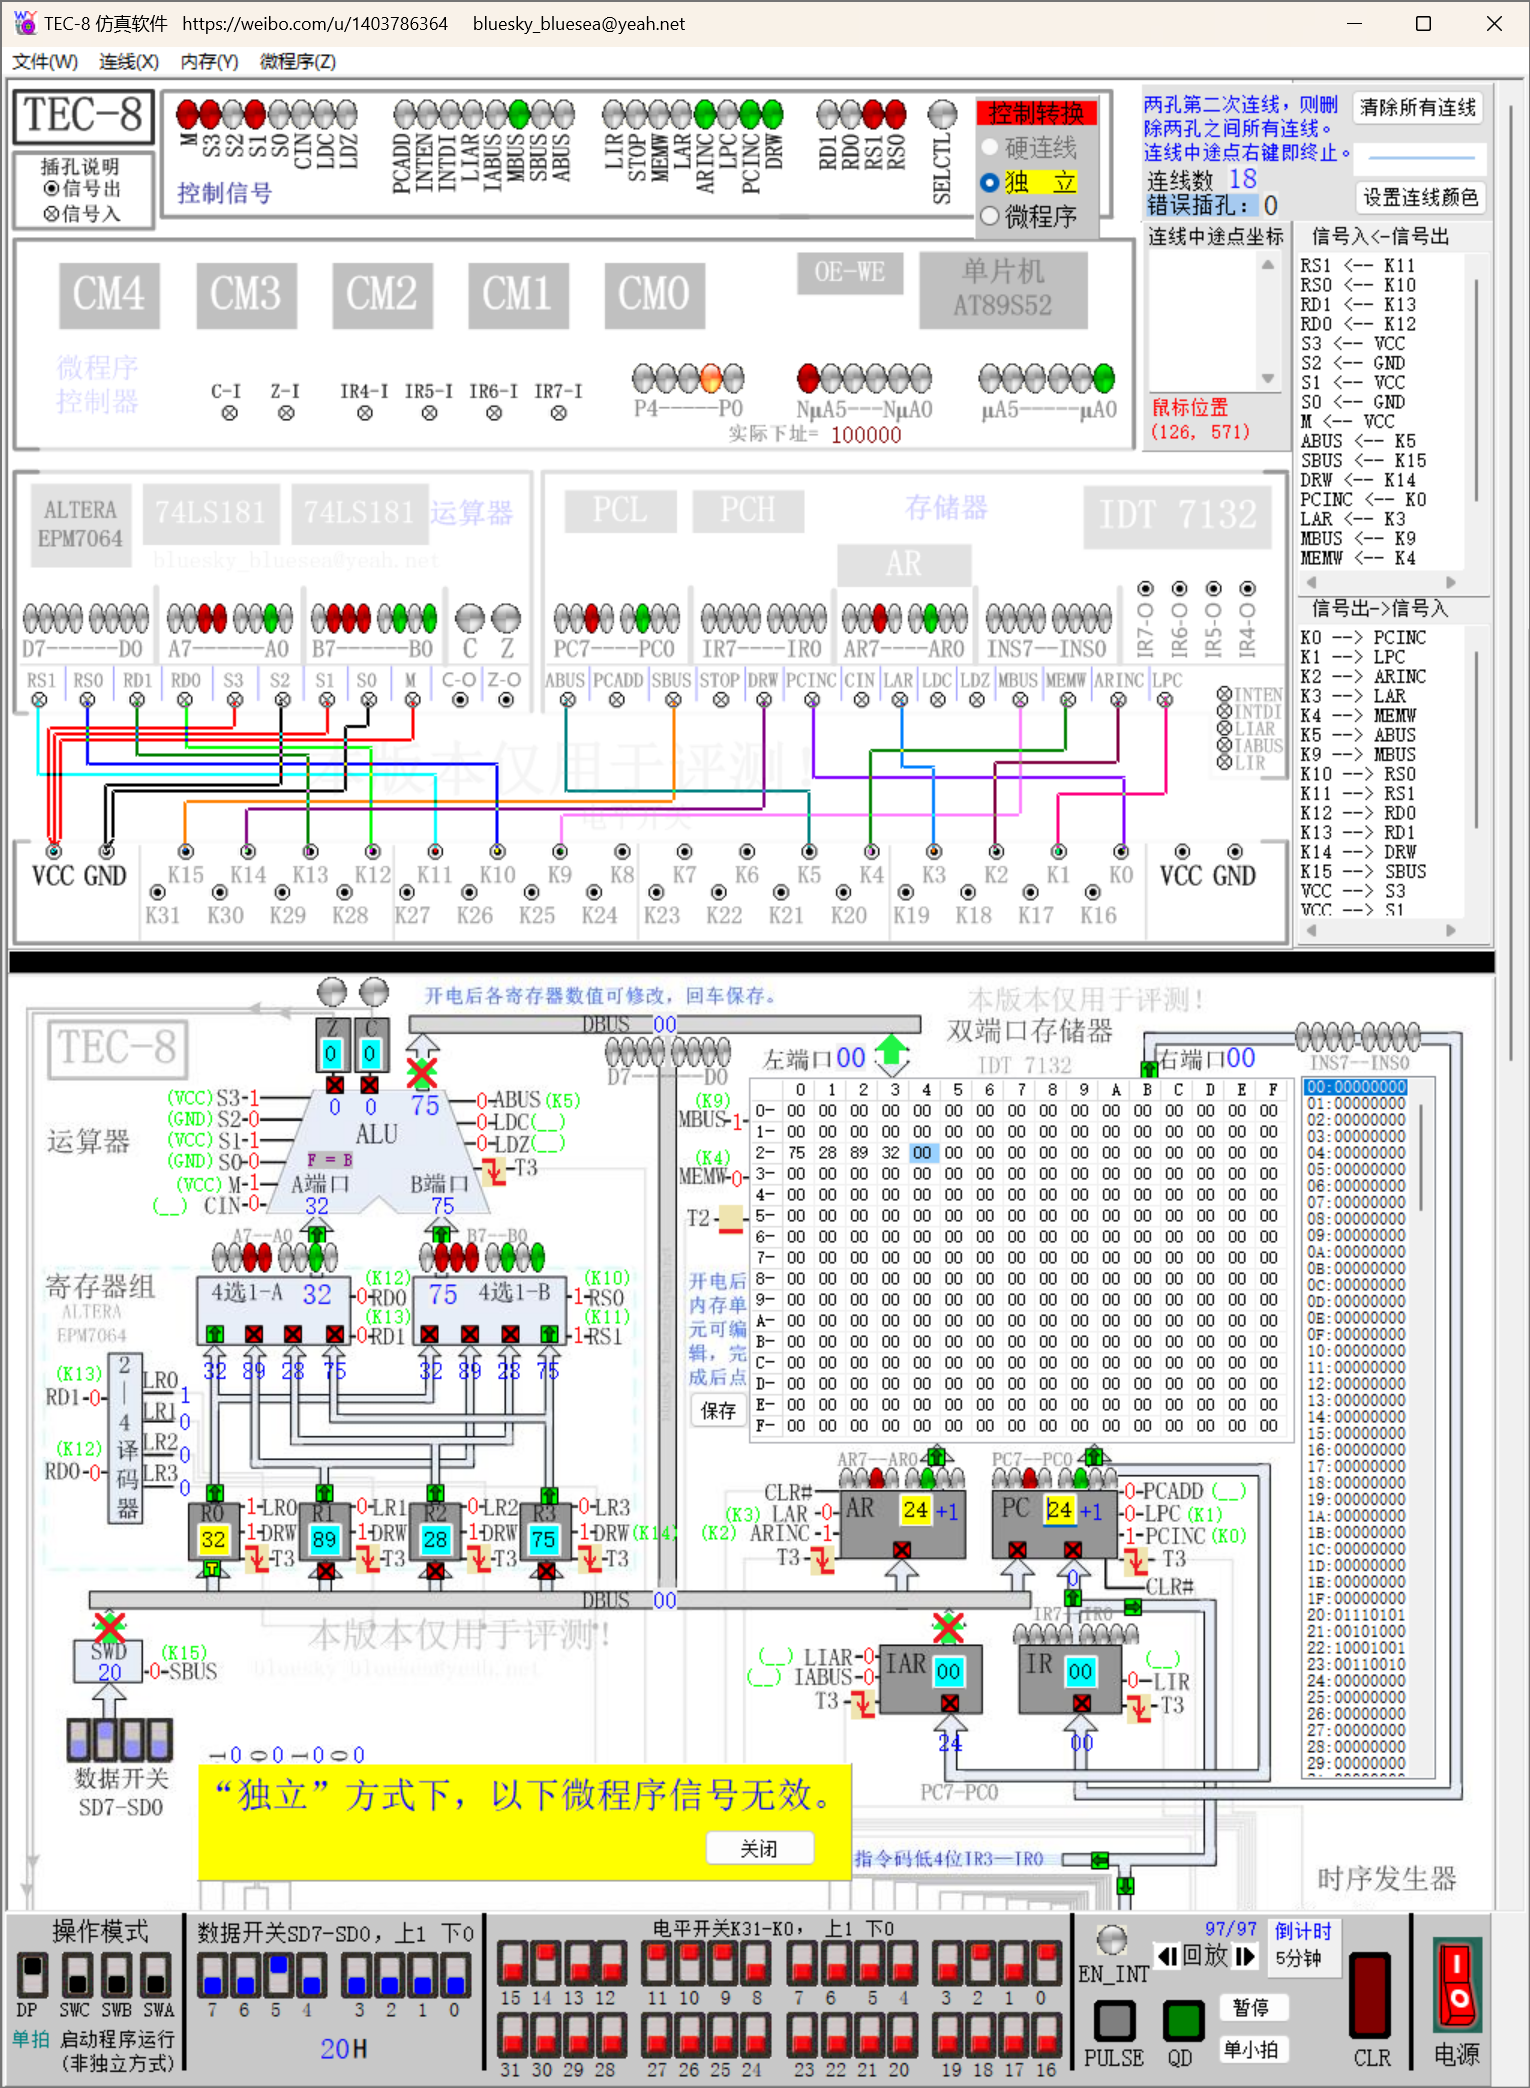
\includegraphics[width=0.3\textwidth]{screenshots/3.2.15.png}
              }
              \caption{写入寄存器 (独立)}
              \label{fig:3.11}
          \end{figure}

\end{enumerate}

\section{思考与心得}

\subsection{思考}

\subsubsection{实验中各个信号的作用}

\begin{itemize}

    \item SBUS, MBUS, ABUS

          三者分别控制数据开关, 存储器, ALU对总线的写入.
          通过数据开关写入数据和设置地址时需要打开SBUS,
          读取存储器数据时需要打开MBUS,
          要从总线获取ALU输出时需要打开ABUS.

    \item LPC, PCINC, LAR, ARINC

          LPC, LAR分别控制PC和AR对总线数据的读取, 设置初始地址时需要打开这两个信号.
          PCINC, ARINC分别控制PC和AR的自增, 实验中对存储器连续区间进行依次读写时需要开启这两个信号.

    \item MEMW

          总线向存储器写入数据时需要打开此信号.

    \item M, S$_{0-3}$, CIN

          控制ALU进行运算的类型. 在实验中需要正确配置这些信号使ALU输出B端口的值.

    \item SEL3, SEL2, SEL1, SEL0

          在输入数据时, 控制输入的数据送入哪个寄存器; 在进行运算时, 控制操作数A, B分别从哪个寄存器获得.
          涉及寄存器操作时要根据要求的地址正确配置这些信号.

\end{itemize}

\subsubsection{数据的流动路径和流动方向}

\begin{enumerate}

    \item 给寄存器置初值

          数据开关$\rightarrow$总线$\rightarrow$寄存器.

    \item 设置存储器地址

          数据开关$\rightarrow$总线$\rightarrow$AR, PC.

    \item 将寄存器中的数写到存储器中

          寄存器$\rightarrow$总线$\rightarrow$存储器.

    \item 从存储器中读数到寄存器

          存储器$\rightarrow$总线$\rightarrow$寄存器.

\end{enumerate}

\subsubsection{如果用 I-cache 和 D-cache 来代替双端口存储器, 请提出一种数据通路方案.}

可以将AR连接至D-cache, PC连接至I-cache, 分数据总线和指令总线完成数据通路.

\subsection{心得}

通过这次实验, 我对寄存器, ALU, 总线, 存储器等计算机组成部件有了更深入的了解.
我也对计算机各种指令进行时的的数据通路有了更深的认识.

\end{document}